% Causal quantum-channel simulation: memory beyond entropy.
% Compile: python build.py (three pdflatex passes).
\documentclass[11pt,a4paper]{article}

\usepackage[utf8]{inputenc}
\usepackage[T1]{fontenc}
\usepackage{lmodern}
\usepackage{amsmath,amssymb,amsthm}
\usepackage[margin=1.1in]{geometry}
\usepackage{booktabs}
\usepackage{enumitem}
\usepackage{microtype}
\setlength{\emergencystretch}{2em}
\usepackage{xcolor}
\usepackage{tikz}
\usetikzlibrary{arrows.meta,calc,positioning,decorations.pathreplacing}
\usepackage{pgfplots}
\pgfplotsset{compat=1.18}
\usepgfplotslibrary{fillbetween}
\usepackage[most]{tcolorbox}
\usepackage[colorlinks=true,linkcolor=blue!50!black,citecolor=blue!50!black,urlcolor=blue!50!black]{hyperref}
\makeatletter
\renewcommand*\l@subsection{\@dottedtocline{2}{1.5em}{3.2em}}
\makeatother
\hypersetup{pdftitle={Causal quantum-channel simulation: memory beyond entropy},
pdfauthor={Seth Douglas and Nidhal Mghirbi},pdfkeywords={quantum channels, factorizable maps, memory, purity, hyperlinear profile, Houghton groups}}

\theoremstyle{plain}
\newtheorem{theorem}{Theorem}[section]
\newtheorem{mainthm}{Theorem}
\renewcommand{\themainthm}{\Alph{mainthm}}
\newtheorem{proposition}[theorem]{Proposition}
\newtheorem{corollary}[theorem]{Corollary}
\newtheorem{lemma}[theorem]{Lemma}
\theoremstyle{definition}
\newtheorem{definition}[theorem]{Definition}
\theoremstyle{remark}
\newtheorem{remark}[theorem]{Remark}

\DeclareMathOperator{\Tr}{Tr}
\DeclareMathOperator{\rank}{rank}
\DeclareMathOperator{\diag}{diag}
\DeclareMathOperator{\Sym}{Sym}
\DeclareMathOperator{\FSym}{FSym}
\DeclareMathOperator{\Ad}{Ad}
\newcommand{\Dmix}{D^{\mathrm{mix}}}
\newcommand{\DChoi}{D^{J}}
\newcommand{\dJ}{d_J}
\newcommand{\ddia}{d_\diamond}
\newcommand{\Dsupp}{\mathfrak{D}}
\title{Causal quantum-channel simulation:\\[3pt]
\large memory beyond entropy}
\author{Seth Douglas \and Nidhal Mghirbi}
\date{September 2026}

\begin{document}
\maketitle

\begin{abstract}
What determines the memory needed to simulate a quantum channel repeatedly, when every output must be released before the next input arrives?
We exhibit two channels on $\mathbb C^{1664}$ with identical normalized Choi spectra: $32$ eigenvalues $1/32$ and all others zero. Both have
maximal complementary entropy $5$, attained at the maximally mixed input, and zero asymptotic purity cost.
At exchange at most $5n/2$ qubits, one has an exact zero-purity implementation with five
memory qubits for arbitrarily many uses; the other requires $\Omega(n^{1/(2\log_2 107+2)})$ memory qubits at every fixed error at most $1/16$, regardless
of the available purity. The latter also admits a zero-purity implementation with memory $O(n^{1/3}\log^{4/3}n)$ at that exchange.

More generally, for sublinear memory and vanishing error, the closed region of exchange and consumed-purity rates $(j,b)$ is
$b\ge\kappa$, $j\ge b$, $2j-b\ge H$, where $H$ is the maximal complementary entropy and $\kappa$ is the closed-device purity cost;
achievability uses the closed-device rate theorem.
We prove that $\kappa$ vanishes exactly on the
closure of finite tracial factorizations and is bounded below by the squared Choi distance to that closure. Within the closure, sequential
support tests and reservoir constructions bound memory through finite-approximation profiles. For channels constructed from finite group
presentations, these bounds translate into quantitative unitary approximation of the fixed list of gadget words. Houghton's group supplies the explicit
separation above; its support-profile exponent lies between $1/(2\log_2 107+1)$ and $1/3$. All operational
bounds use complete-experiment error against adaptive observers with quantum references.
\end{abstract}

\tableofcontents
\clearpage

%======================================================================
\section{Introduction}\label{sec:intro}
%======================================================================

\paragraph{The question.} A unitary channel can be applied again and again by the same device at no cost. A general channel
$\Phi$ cannot: each use entangles the input with an environment, and a device that is to act as $\Phi$ on the next input as well
must either carry that environment along or hand it off. Ryb\'ar and Ziman called a channel \emph{repeatable} when a single memory
device implements it on each individual input~\cite{RybarZiman2008}, and showed that random-unitary channels are repeatable
while nonunital ones are not. In the closed setting, where nothing may be exchanged with the outside, the bath dimension and
initial entropy required per use were characterized in~\cite{Douglas2026closed}.

Here we study the open setting (Figure~\ref{fig:service}). A device receives $n$ inputs in sequence, applies a fixed public
protocol, and releases each output before the next input arrives. Between uses it may export registers permanently and import
fresh independent ones. The whole experiment must be within a small error~$\epsilon$ of $n$ independent uses of $\Phi$, against an
arbitrary adaptive observer who chooses each input after seeing the earlier outputs and keeps quantum references
(Definition~\ref{def:service}). We count three resources: the retained memory, the exchange, and the purity the device starts with or
imports (see the box below). Exchange at rate $H(\Phi)/2$, half the maximal complementary entropy, is necessary for vanishing error
with sublinear memory and purity (Proposition~\ref{prop:exchange}). The questions are how much purity and how much memory the
device then needs, and what decides it.

\begin{figure}[htbp]
\centering
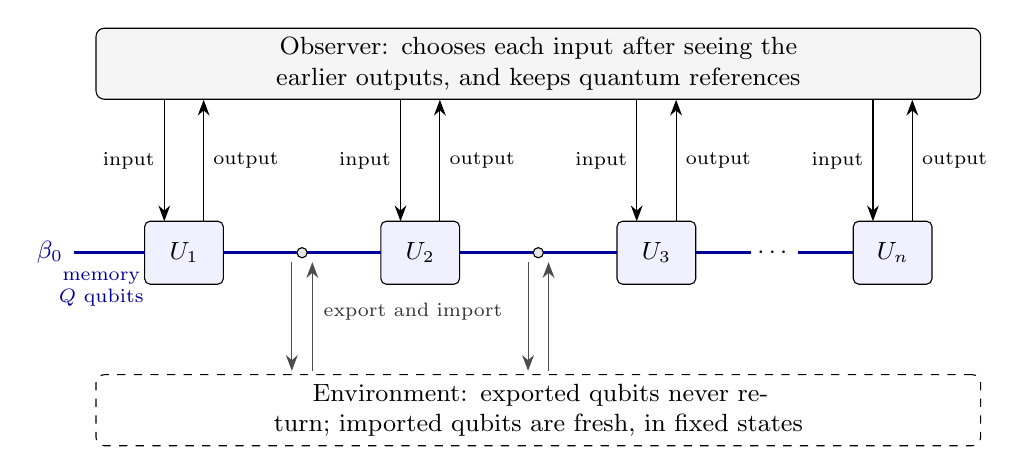
\begin{tikzpicture}[font=\small,>={Stealth[length=2mm]},
  rnd/.style={draw,rounded corners=2pt,minimum width=1.0cm,minimum height=0.8cm,fill=blue!6},
  ex/.style={draw,circle,inner sep=1.3pt,fill=gray!20}]
\node[draw,rounded corners=3pt,fill=gray!8,text width=11cm,align=center,minimum height=0.7cm] (obs) at (4.5,2.4)
  {Observer: chooses each input after seeing the earlier outputs, and keeps quantum references};
\foreach \x/\lab in {0/{U_1},3/{U_2},6/{U_3},9/{U_n}} {
  \node[rnd] at (\x,0) {$\lab$};
  \draw[->] (\x-0.25,0 |- obs.south) -- node[left]{\scriptsize input} (\x-0.25,0.4);
  \draw[->] (\x+0.25,0.4) -- node[right]{\scriptsize output} (\x+0.25,0 |- obs.south);
}
\draw[very thick,blue!60!black] (-1.4,0) node[left]{$\beta_0$} -- (-0.5,0);
\draw[very thick,blue!60!black] (0.5,0) -- (2.5,0);
\draw[very thick,blue!60!black] (3.5,0) -- (5.5,0);
\draw[very thick,blue!60!black] (6.5,0) -- (7.2,0);
\node at (7.5,0) {$\cdots$};
\draw[very thick,blue!60!black] (7.8,0) -- (8.5,0);
\node[ex] at (1.5,0) {};
\node[ex] at (4.5,0) {};
\node[blue!60!black,anchor=north,align=center,font=\scriptsize] at (-1.05,-0.12) {memory\\$Q$ qubits};
\node[draw,dashed,rounded corners=3pt,text width=11cm,align=center,minimum height=0.6cm] at (4.5,-2.0)
  {Environment: exported qubits never return; imported qubits are fresh, in fixed states};
\foreach \x in {1.5,4.5} {
  \draw[->,gray!60!black] (\x-0.13,-0.12) -- (\x-0.13,-1.5);
  \draw[->,gray!60!black] (\x+0.13,-1.5) -- (\x+0.13,-0.12);
}
\node[gray!40!black,anchor=west] at (1.65,-0.75) {\scriptsize export and import};
\end{tikzpicture}
\caption{Causal service of a channel for $n$ rounds. The memory (thick line) starts in a fixed state $\beta_0$. In each round a
fixed unitary $U_t$ acts on the fresh input and the memory, and the output is released at once. Between rounds some memory
qubits are exported for good and replaced by fresh imports. The observer may adapt each input to everything seen so far.}
\label{fig:service}
\end{figure}

\begin{tcolorbox}[colback=gray!4,colframe=gray!45,boxrule=0.5pt,arc=2pt,left=6pt,right=6pt,top=4pt,bottom=4pt,
  title={\small The resource ledger},fonttitle=\bfseries,coltitle=black,colbacktitle=gray!15]
\small
\begin{itemize}[leftmargin=1.2em,itemsep=2pt,topsep=2pt]
\item \emph{Error} $\epsilon$: the largest trace distance, over adaptive observers with quantum references, between the whole
experiment and $n$ independent uses of $\Phi$.
\item \emph{Memory} $Q$: every retained qubit, including clocks, padding and workspace.
\item \emph{Exchange} $J$: the number of qubits exported, which equals the number imported. Imports happen between rounds; the qubits
imported in one step form a register in a fixed state, independent of everything else.
\item \emph{Purity}: the initial deficit $P=Q-S(\beta_0)$ plus the imported deficit $C$, the sum over imports of qubits minus
entropy. A purity budget $B$ means $P+C\le B$.
\item $H(\Phi)$ is the maximal complementary entropy. With sublinear memory and purity, exchange at rate $H(\Phi)/2$ is necessary (such
services exist only on the closure class, where $\kappa=0$); with sublinear memory alone, the least rate is $(H(\Phi)+\kappa(\Phi))/2$. There is no free reset, postselection or measurement
record. Logarithms are to base two.
\end{itemize}
\end{tcolorbox}

\paragraph{The answer in brief.} Let $\mathcal K_d$ be the closure of the channels on $M_d$ of the form
$\rho\mapsto(\mathrm{id}\otimes\tau_m)[U(\rho\otimes I_m)U^*]$, with $U$ unitary and $\tau_m$ the normalized trace, and call such channels \emph{exact
factors}. At leading order, exchange and purity are set jointly by $H$ and by the closed-device cost $\kappa$ of~\cite{Douglas2026closed}: with
sublinear memory and vanishing error the least exchange rate is $(H+\kappa)/2$ and the least purity rate is $\kappa$
(Corollary~\ref{cor:exchange-purity}). The cost $\kappa$ vanishes exactly on $\mathcal K_d$, so purity decides whether a channel is a limit of exact
factors, and on $\mathcal K_d$ the exchange threshold is $H/2$. Memory measures what neither $H$ nor $\kappa$ records: how hard the channel is to
approximate.

The sharpest comparison also matches the complete single-use Choi spectrum. Write $Z_D=\diag(e^{2\pi ij/D})_{j=0}^{D-1}$ and
$\Xi_*(X)=\frac1{32}\sum_{a=0}^{31}Z_{1664}^aXZ_{1664}^{-a}$. Section~\ref{sec:flat-choi-proof} constructs a second explicit channel $\Omega$ by
appending diagonal blocks to two copies of the Houghton gadget and balancing the weights of its group labels.

\begin{mainthm}[Memory beyond the Choi spectrum]\label{thm:flat-choi-separation}
The channels $\Xi_*$ and $\Omega$ on $M_{1664}$ have identical normalized Choi spectra, with $32$ eigenvalues $1/32$ and all others zero.
Both have maximal complementary entropy $5$, attained at the maximally mixed input, and lie in $\mathcal K_{1664}$, so both have
$\kappa=0$ and optimal exchange rate $\frac52$. Put $\beta_H=1/(2\log_2 107+1)$.
At exchange $J\le\frac52n$:
\begin{enumerate}[label=(\alph*)]
\item $\Xi_*$ has a causal service with error $0$, $Q=5$ and $P=C=0$ for every $n\ge1$;
\item every causal service of $\Omega$ with error $\epsilon\le1/16$ has $Q=\Omega(n^{1/(2\log_2 107+2)})$, whatever its purity, and
for every fixed $A\ge0$, $Q\ge c_{A+3}(n/\log(n+1))^{\beta_H}-\frac{33}{8}$ if $P+C\le A\log(n+1)$,
where $c_A$ is defined after Theorem~\ref{thm:constant-lower};
\item for every $n\ge1$ and $0<\epsilon\le1$, $\Omega$ has a causal service with error $\epsilon$, $P=C=0$ and
$Q=O((n/\epsilon)^{1/3}\log^{4/3}(2n/\epsilon))$.
\end{enumerate}
Above that exchange, with excess $E_{\rm x}=(J-\frac52n)_+$, every service of $\Omega$ with error $\epsilon\le1/16$ satisfies the bound of
Corollary~\ref{cor:purity}(d) with $Q+4$ in place of $Q$; so the separation survives an excess exchange of $O(n^\gamma)$ for every $\gamma<1$.
\end{mainthm}

The proof is in Section~\ref{sec:flat-choi-proof}. The lower and upper memory exponents do not match: the theorem separates memory costs,
not their exact asymptotic laws. A smaller pair on $M_{208}$ matches Choi rank, maximal complementary entropy, its optimal spectrum, and purity
cost, but not the full Choi spectrum (Corollary~\ref{cor:208}).
More generally, Proposition~\ref{prop:spectrum-completion} completes any group gadget to a flat-Choi-spectrum channel while retaining it
as an invariant corner. This preserves its memory obstruction up to a fixed tag cost, and preserves finite-factor-closure membership in
both directions; the construction above reduces the system dimension to $1664$, without a minimality claim.

\paragraph{Dependencies of Theorem~\ref{thm:flat-choi-separation}.}
The lower bound starts with the weighted group obstruction supplied by the companion paper~\cite{DouglasMghirbiA}
(Section~\ref{sec:imported}), then uses the sequential extraction proved here to obtain the Houghton memory bound
(Theorem~\ref{thm:constant-lower}). The flat-probe purity estimate (Theorem~\ref{thm:rank-purity}) makes that obstruction independent of a
separate purity budget at the stated exchange. Spectrum completion and a recyclable corner tag transfer it to $\Omega$
(Section~\ref{sec:flat-choi-proof}). For the upper bound, the companion's smoothed group models give full-Choi approximants here,
to which the rank-rate compiler (Theorem~\ref{thm:rank-rate}) applies. The closed-device achievability theorem
of~\cite{Douglas2026closed}, used for the general rate region, is not an input to these two explicit service constructions or their memory separation.

\paragraph{Why the spectra can agree.}
The original gadget has $26$ mutually orthogonal system coefficient matrices $K_g$, but unequal squared Frobenius norms $\mu_g$.
Two copies make every $2\mu_g$ integral. Adding $52-2\mu_g$ scalar blocks for each old group label and $52$ for each of six new labels
makes all $32$ norms equal to $52$, in total dimension $32\cdot52=1664$.
Orthogonality then gives the common Choi spectrum, while an untouched $104$-dimensional corner still acts as $\Phi_H$.
Four retained pure qubits suffice to select and recycle that corner: they add four to memory and initial purity, not a fresh cost per call.
The lower bound applies the flat-probe purity estimate to the completed channel, then transfers to this corner. The upper bound combines
the second-order Choi approximants with the rank-rate compiler. This is why matching a full Choi spectrum does not erase the obstruction.

The underlying example is a channel $\Phi_H$ on $\mathbb C^{104}$ built from Houghton's group (Section~\ref{sec:houghton}). It has the same
Choi rank $26$, entropy $\log26$, flat optimal complementary spectrum and zero purity cost as the exact factor
$\Phi_0=\mathrm{id}_4\otimes\Delta_{26}$, where $\Delta_{26}$ is complete dephasing. At their optimal exchange rate, $\Phi_0$ needs only
$O(\log n)$ memory, while $\Phi_H$ needs at least order $(n/\log n)^{1/14.48}$ at logarithmic purity and at most
$O(n^{1/3}\log^{4/3}n)$ (Theorem~\ref{thm:intro-lower}).
Table~\ref{tab:glance} collects the bounds.

\begin{table}[t]
\centering
\small
\begin{tabular}{@{}p{3.5cm}p{8.2cm}p{2.1cm}@{}}
\toprule
Channel & Purity and memory for $n$ uses & Where\\
\midrule
Any channel & least purity rate at vanishing error $\kappa(\Phi)$, which is $0$ exactly on $\mathcal K_d$ and at least
$\Delta_J(\Phi)^2/(2\ln2)$ off it; least exchange rate $(H+\kappa)/2$ with sublinear memory; outside $\mathcal K_d$, linear memory at rate $H/2$ &
Thm~\ref{thm:purity}, Cor~\ref{cor:exchange-purity}\\
Exact factor & memory $O(\log n)$ at exchange $H/2+s$ and at the rank rate $\frac12\log r$; at the optimal rate $H/2$, $O(\log n)$
if the complementary spectrum is flat, and between order $\sqrt n$ and $\sqrt{n\log n}$ if not & Thms~\ref{thm:upper}, \ref{thm:rank-exact}\\
Any channel in $\mathcal K_d$ & memory between the one-round profile at leakage about $(\log n)/n$ and the Choi profile at accuracy
$\epsilon/(8dn)$ & Thms~\ref{thm:sequential}, \ref{thm:closure-upper}, \ref{thm:rank-rate}\\
Gadget channel of a group & memory between the group's approximation profile at relator defect about $(\log n/n)^{1/4}$ and about
$(n\log n)^{-1/2}$; if $\Phi_G\in\mathcal K_d$, the upper bound at the optimal rate & Thm~\ref{thm:group-bracket}\\
Houghton channel $\Phi_H$ & in $\mathcal K_{104}$, $H=\log26$; memory between $(n/\log n)^{\beta_H}$, $\beta_H\approx1/14.48$, and
$n^{1/3}\log^{4/3}n$, the upper bound at the optimal rate & Thm~\ref{thm:constant-lower}, Cor~\ref{cor:third}\\
Slofstra channel $\Phi_S$ & memory at least $n^{1/8-o(1)}$, whichever side of $\mathcal K_d$ it lies on; at its rank rate at least $n^{1/9-o(1)}$
whatever the purity, and linear if $\Phi_S\notin\mathcal K_d$ & Thm~\ref{thm:slofstra}\\
\bottomrule
\end{tabular}
\caption{Results at a glance, at constant error and a logarithmic purity budget unless stated. The nonflat exact-factor lower bound requires
sufficiently small fixed error as in Corollary~\ref{cor:flat-split}(b). $H$ is the maximal complementary entropy and $r$ the Choi rank.}
\label{tab:glance}
\end{table}

\paragraph{Purity marks the closure.} The general framework starts with the purity cost. It is the closed-device cost $\kappa$
of~\cite{Douglas2026closed}, a smoothed conditional entropy of one use (Section~\ref{sec:res-purity}), and it detects the closure class.

\begin{mainthm}[Purity; Theorem~\ref{thm:purity} and Proposition~\ref{prop:discontinuity}]\label{thm:intro-purity}
For every channel $\Phi$ on $M_d$ the least purity rate $\lim(P+C)/n$ of causal services with vanishing error is $\kappa(\Phi)$. It satisfies
$\kappa(\Phi)\ge\Delta_J(\Phi)^2/(2\ln2)$, where $\Delta_J$ is the Choi distance to $\mathcal K_d$, and it vanishes exactly on $\mathcal K_d$; every service
with error $\epsilon$ has $P+C\ge n(\Delta_J(\Phi)-\epsilon)_+^2/(2\ln2)$, at any exchange and with any memory. With sublinear memory the least exchange rate
is $(H(\Phi)+\kappa(\Phi))/2$, so outside $\mathcal K_d$ memory is linear at the entropy rate $H/2$ (Corollary~\ref{cor:exchange-purity}). But $\kappa$ is not
continuous at $\mathcal K_d$: there are qubit channels with $\Delta_J\to0$ and $\kappa=1$.
\end{mainthm}

Inside $\mathcal K_d$, zero-purity services exist at every fixed error and horizon at the rank rate (Theorem~\ref{thm:rank-rate}).
Outside it the purity cost is linear, even for channels realized
exactly by a tracial von Neumann algebra: the negative answer to Connes' embedding problem~\cite{JNVWY2020}, through a theorem of Haagerup and
Musat~\cite{HaagerupMusat2015}, gives a generally factorizable channel outside $\mathcal K_d$ (Corollary~\ref{cor:connes}). So purity separates finite
approximability from its failure. It cannot see the structure inside $\mathcal K_d$, where $\kappa=0$; memory can.

\paragraph{Memory inside the closure.} Exact factors need little memory. At every exchange rate above the optimum, and at the rank rate
$\frac12\log r$ with $r$ the Choi rank, memory $O(\log(n/\epsilon))$ suffices (Theorems~\ref{thm:upper} and~\ref{thm:rank-exact}). At the optimal rate itself the
answer depends on one spectrum: when the complementary output of an optimal input is flat, the optimal rate is the rank rate and memory stays
logarithmic; when it is not, memory of order $\sqrt n$ is necessary at small fixed error, and order $\sqrt{n\log n}$ suffices
(Corollary~\ref{cor:flat-split}).

For limits of exact factors the memory is bracketed by how large a finite realization must be to approximate one use to accuracy about $1/n$.
For full-Choi-rank targets and fixed positive exchange slack, the upper bound improves this scale to $1/\sqrt n$
(Corollary~\ref{cor:fullrank-service}).

\begin{mainthm}[The bracket; Theorems~\ref{thm:sequential}, \ref{thm:closure-upper} and~\ref{thm:rank-rate}]\label{thm:intro-law}
Let $\Phi$ be a channel on $M_d$ and $0<\epsilon<1/2$.
\begin{enumerate}[label=(\alph*)]
\item Every causal service of $\Phi$ for $n$ rounds with error $\epsilon$ and purity budget $B$ has, at any exchange,
\[
Q\ \ge\ \log D^{\mathrm{ent}}_\Phi\Big(\frac{\epsilon}{1-\epsilon},\,t_n\Big),\qquad t_n=\frac{B+\epsilon+h_2(\epsilon)+\epsilon\log n}{n(1-\epsilon)}.
\]
\item If $\Phi\in\mathcal K_d$, put $m=\DChoi_\Phi(\epsilon/(8dn))$ and $x=\log(256n/\epsilon)$.
For $0<s\le1$ and $x<n$, there is a service with error $\epsilon$, $P=C=0$,
$Q\le\log m+\log(2+\log m)+O_d(x/s+\log(n+1))$ and exchange at most $n(H(\Phi)/2+s)$.
For every horizon there is also a service with error $\epsilon$, $P=C=0$ and
$Q\le\log m+\log(2+\log m)+O_d(\log^2(n/\epsilon))$ at the rank rate $\frac n2\log r$.
\end{enumerate}
\end{mainthm}

Here $D^{\mathrm{ent}}_\Phi(u,v)$ is the least bath dimension of one use, with any bath state, that is within diamond distance $u$ of $\Phi$ and whose
support leakage plus entropy production is at most $v$, and $\DChoi_\Phi(\delta)$ is the least bath dimension of an exact factor within Choi distance
$\delta$ (Figure~\ref{fig:bracket}).

\paragraph{Memory reads the group.} Many channels in $\mathcal K_d$ come from groups. Every finite presentation $\mathcal P$ of a group $G$ gives a
\emph{gadget channel} $\Phi_G$, built from unitary $2\times2$ blocks that record the multiplication of the relators' prefixes and evaluated in the
regular representation (Section~\ref{sec:res-group}). Its profiles and the approximation profile $\mathsf h_{\mathcal P}(e,z)$ of the presentation (the least
dimension of unitaries with relator defect $e$ and error $z$ on the moments of finitely many words) bound each other up to polynomial changes of
scale, and $\Phi_G\in\mathcal K_d$ exactly when $\mathsf h_{\mathcal P}$ is finite everywhere (Theorem~\ref{thm:correspondence}).

\begin{mainthm}[Group channels; Proposition~\ref{prop:gadget-entropy} and Theorem~\ref{thm:group-bracket}]\label{thm:intro-group}
Every gadget channel has maximal complementary entropy $\log r$, with $r$ its Choi rank, so its entropy rate is its rank rate, and this is its
optimal exchange rate when $\Phi_G\in\mathcal K_d$. At constant error and logarithmic purity, the least memory of $n$ uses of $\Phi_G$ is at least
$\log\mathsf h_{\mathcal P}$ at relator defect of order $(\log n/n)^{1/4}$, up to $O(\log n)$, and, if $\Phi_G\in\mathcal K_d$, at most $O(\log n)$ times
$\log\mathsf h_{\mathcal P}$ at relator defect of order $(n\log n)^{-1/2}$, plus $O(\log^2n)$, at the rank rate. At the rank rate the lower bound holds
whatever the purity, with the budget replaced by $14Q+3$.
\end{mainthm}

The two bounds read the profile at different scales, roughly $e$ and $e^2$. When $\log\mathsf h_{\mathcal P}$ is a power of $1/e$ this fixes the growth exponent of
the memory up to a factor of $2$; for general profiles it brackets the memory between two readings of the same function. Groups with steep
profiles give channels that need polynomial memory.

\paragraph{The Houghton channel.} Houghton's group $H_3$~\cite{Houghton1978} is finitely presented and amenable, and the companion paper~\cite{DouglasMghirbiA} shows that
approximate representations of a finite piece of it need stretched-exponential dimension. Its gadget channel $\Phi_H$ acts on $\mathbb C^{104}$, has
Choi rank $26$ and $H(\Phi_H)=\log26$, and lies in $\mathcal K_{104}$, so $\kappa(\Phi_H)=0$.

\begin{mainthm}[Polynomial memory in the closure; Theorems~\ref{thm:constant-lower}, \ref{thm:rank-purity} and Corollary~\ref{cor:third}]\label{thm:intro-lower}
Fix $0<\epsilon\le1/16$ and $A\ge4$, and put $\beta_H=1/(2\log107+1)\approx1/14.48$.
\begin{enumerate}[label=(\alph*)]
\item Every causal service of $\Phi_H$ for $n$ rounds with error $\epsilon$ and $P+C\le A\log(n+1)$ has, at any exchange,
$Q\ge c_A(n/\log(n+1))^{\beta_H}-\frac18$.
\item At the optimal exchange $J\le\frac n2\log26$, every causal service with error $\epsilon$ has $Q=\Omega(n^{1/(2\log107+2)})$, whatever its purity.
\item There is a causal service with error $\epsilon$, $J\le\frac n2\log26$, $P=C=0$ and $Q=O(n^{1/3}\log^{4/3}n)$.
\end{enumerate}
\end{mainthm}

This is the comparison with $\Phi_0=\mathrm{id}_4\otimes\Delta_{26}$ above: the two channels agree in every invariant that sets exchange or purity, and
their memory differs polynomially. Entropy does not price memory.

\paragraph{A Slofstra channel.} Slofstra's finitely presented group~\cite{Slofstra2018} has a steeper profile, and it is not known whether it is
hyperlinear. Its gadget channel, after one Tietze move, needs memory $n^{1/8-o(1)}$ at logarithmic purity, and $n^{1/9-o(1)}$ at its rank rate
whatever its purity. Either it lies in $\mathcal K_d$, or its purity cost is linear, its memory at the rank rate is linear, and the group is not
hyperlinear (Theorem~\ref{thm:slofstra}).

\begin{figure}[t]
\centering
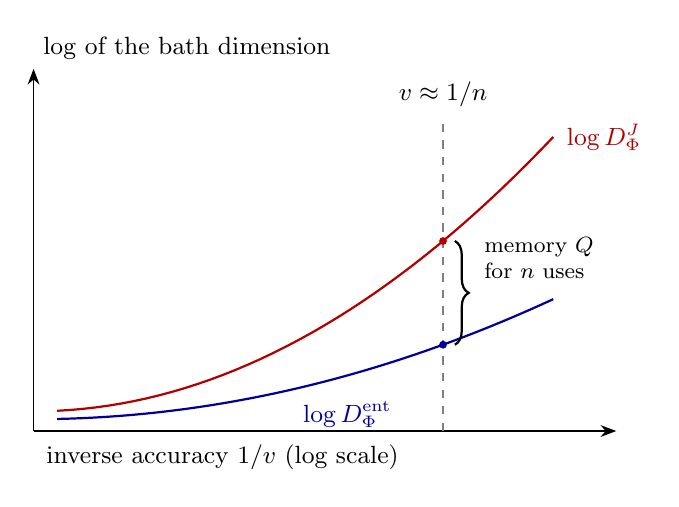
\begin{tikzpicture}[font=\small,>={Stealth[length=2mm]}]
\draw[->] (0,0) -- (7.4,0);
\node[below] at (2.4,-0.05) {inverse accuracy $1/v$ (log scale)};
\draw[->] (0,0) -- (0,4.6) node[above right]{$\log$ of the bath dimension};
\draw[thick,red!70!black,domain=0.3:6.6,samples=40] plot (\x,{0.08*\x*\x+0.25});
\node[red!70!black,anchor=west] at (6.65,3.73) {$\log\DChoi_\Phi$};
\draw[thick,blue!60!black,domain=0.3:6.6,samples=40] plot (\x,{0.035*\x*\x+0.15});
\node[blue!60!black,anchor=north west] at (3.3,0.5) {$\log D^{\mathrm{ent}}_\Phi$};
\draw[dashed,gray] (5.2,0) -- (5.2,4.0) node[above,black]{$v\approx1/n$};
\draw[decorate,decoration={brace,amplitude=5pt,mirror},thick] (5.35,1.096) -- (5.35,2.413);
\node[anchor=west,align=left,font=\footnotesize] at (5.6,2.2) {memory $Q$\\for $n$ uses};
\fill[blue!60!black] (5.2,1.096) circle (1.4pt);
\fill[red!70!black] (5.2,2.413) circle (1.4pt);
\end{tikzpicture}
\caption{Theorem~\ref{thm:intro-law} in a picture. The memory for $n$ uses lies between two profiles read at accuracy about $1/n$: below, the
one-round profile, which allows biased bath states and measures leakage; above, the Choi profile of single exact factors. For $\Phi_H$ the one-round
profile at distance $1/8$ is between $\exp(c\,v^{-\beta_H})$ and $\exp(O(v^{-1/3}))$ (Proposition~\ref{prop:smoothed}), and the Choi profile is at most
$\exp(O(v^{-1/3}\log^{4/3}(1/v)))$ (Theorem~\ref{thm:choi-profile}).}
\label{fig:bracket}
\end{figure}

\paragraph{How the proofs go.}
\begin{itemize}[leftmargin=1.2em,itemsep=2pt]
\item \emph{Purity} (Section~\ref{sec:purity}). Each round of a service, fed a fixed input, is a feasible extension in the definition of $\kappa$, and its
entropy production is paid from the purity budget. A tracialization lemma turns small entropy production into a nearby finite tracial mixture.
\item \emph{One round reads the profile} (Section~\ref{sec:bridge}). An observer tests every output against the support of the Choi state, which the
ideal passes with certainty; an entropy ledger then finds a round whose leakage and entropy production are both of order $(\log n)/n$.
\item \emph{Groups} (Section~\ref{sec:group-channels}). From a round close to a gadget channel one reads off, block by block, unitaries that satisfy the
relators approximately and reproduce the moments; conversely approximate representations assemble into gadgets, and tensor powers with complex
conjugates sharpen the moments.
\item \emph{Houghton} (Sections~\ref{sec:houghton} to~\ref{sec:constant}). The lower bound combines the one-round extraction with the dimension bounds of the
companion paper. The upper bounds come from permutation models on a clock torus that fail at a single corner, and from unitary models that spread
that defect thinly, which approximate $\Phi_H$ to second order in Choi distance.
\item \emph{Services} (Sections~\ref{sec:sublinear} and~\ref{sec:upper}). A rolling reservoir with a Haar-random bath mixer serves every exact factor. At the rank
rate a pinching bound on R\'enyi entropies replaces the entropy fluctuations that otherwise fix the buffer.
\end{itemize}

\paragraph{Related work.} Repeated use of one device was introduced by Ryb\'ar and Ziman~\cite{RybarZiman2008}; the closed version of our resource count,
with no exchange, is settled in~\cite{Douglas2026closed}, and Theorem~\ref{thm:purity} completes an equivalence left open there. Memory effects across
uses~\cite{Zammit2025} and sequential realizations of instruments~\cite{SauSedlak2025} concern different tasks. Block simulations of $\Phi^{\otimes n}$, by
communication with free entanglement in the quantum reverse Shannon theorem~\cite{BDHSW2014,BCR2011} or by work in the thermodynamic
capacity~\cite{FBB2019}, price other resources and have no causal release; the rank arguments behind our exchange converses parallel the
second-order asymptotics of hypothesis testing~\cite{TomamichelHayashi2013,Li2014}.

Factorizable maps were introduced by Anantharaman-Delaroche~\cite{AD2006}. Haagerup and Musat related them to the Connes embedding
problem~\cite{HaagerupMusat2011,HaagerupMusat2015}, and Musat and R{\o}rdam found factorizable channels that need an infinite-dimensional ancilla and showed that
the finite-ancilla class is not closed~\cite{MusatRordam2020}; see Musat's survey~\cite{Musat2025} and, for synchronous correlations,
Russell~\cite{Russell2019}. These results are qualitative; the profiles here quantify the ancilla dimension as a function of accuracy, and the memory
of repeated use reads them. Quantitative approximation of groups is surveyed in~\cite{ArzhantsevaCherix2020}; the sofic profile is
Cornulier's~\cite{Cornulier2013}, the hyperlinear profile and its relation to nonlocal games are studied in~\cite{SlofstraVidick2018,Slofstra2018}, and
hyperlinear approximations of amenable groups come from sofic ones~\cite{BCJM2023}. The diffusive picture behind one of our services is the classical
link between amenability and random walks~\cite{Kesten1959}.

\paragraph{Organization.} Section~\ref{sec:setting} sets up channels, profiles and the service contract, and Section~\ref{sec:results} states all results in
full. Section~\ref{sec:houghton} introduces the Houghton channel and its finite models, and states what we use from~\cite{DouglasMghirbiA}.
Sections~\ref{sec:extraction} to~\ref{sec:constant} prove the lower bounds, with the purity results in Section~\ref{sec:purity}; Sections~\ref{sec:sublinear}
and~\ref{sec:upper} prove the upper bounds; Section~\ref{sec:group-channels} treats group channels; Section~\ref{sec:open} discusses open problems.

\section{Setting}\label{sec:setting}
%======================================================================

\paragraph{Channels and distances.} All channels act on $M_d=M_d(\mathbb{C})$ for a fixed $d$. For a channel
$\Psi$ write $\mathcal{J}(\Psi)=(\Psi\otimes\mathrm{id})(|\Omega\rangle\langle\Omega|)$ for its normalized Choi
state, with $|\Omega\rangle=d^{-1/2}\sum_i|ii\rangle$, and put
$\dJ(\Psi,\Psi')=\tfrac12\|\mathcal{J}(\Psi)-\mathcal{J}(\Psi')\|_1$ and $\ddia(\Psi,\Psi')=\tfrac12\|\Psi-\Psi'\|_\diamond$.
Logarithms are base two unless written $\ln$. On $M_m$ we use the normalized trace $\tau_m$ and the norms
$\|X\|_{2}=\tau_m(X^*X)^{1/2}$ and $\|X\|_{1}=\tau_m|X|$. We have
\begin{equation}\label{eq:dJ-ddia}
\dJ(\Psi,\Phi)\le\ddia(\Psi,\Phi)\le d\,\dJ(\Psi,\Phi):
\end{equation}
a pure input with any reference has the form $(I\otimes A)|\Omega\rangle$ with $\|A\|_\infty^2\le d$, and
$\|AXB\|_1\le\|A\|_\infty\|X\|_1\|B\|_\infty$.

\begin{definition}[Tracial factorizations and profiles]\label{def:profile}
A channel $\Psi$ on $M_d$ has a \emph{finite tracial factorization with bath dimension $m$} if
$\Psi(\rho)=(\mathrm{id}\otimes\tau_m)\big[U(\rho\otimes I_m)U^*\big]$ for a unitary $U$ on
$\mathbb{C}^d\otimes\mathbb{C}^m$. Let $\mathcal{F}_m$ be the set of finite convex combinations of such channels whose
components have bath dimension at most $m$. For a channel $\Phi$ define
\begin{align*}
\DChoi_\Phi(\delta)&=\min\{m:\ \exists\,\Psi \text{ with a factorization of bath dimension }m,\ \dJ(\Psi,\Phi)\le\delta\},\\
\Dmix_\Phi(\delta)&=\min\{m:\ \exists\,\Psi\in\mathcal{F}_m,\ \dJ(\Psi,\Phi)\le\delta\}.
\end{align*}
Clearly $\Dmix\le\DChoi$. The \emph{closure class} consists of channels with $\DChoi(\delta)<\infty$ for every
$\delta>0$.
\end{definition}

\begin{definition}[Support-sensitive profile]\label{def:support-profile}
Let $\Pi_\Phi$ be the support projection of $\mathcal J(\Phi)$ and define the \emph{support leakage}
$\ell_\Phi(\Psi)=\mathrm{Tr}[(I-\Pi_\Phi)\mathcal J(\Psi)]$. Put
\[
\Dsupp_\Phi(u,v)=\min\{m:\ \exists\,\Psi\in\mathcal F_m,\ \ddia(\Psi,\Phi)\le u,\ \ell_\Phi(\Psi)\le v\}.
\]
\end{definition}

Since $\mathrm{Tr}[PX]\le\frac12\|X\|_1$ for a projection $P$ and a traceless Hermitian $X$, the leakage changes by at
most $\dJ$ under a change of channel, and~\eqref{eq:dJ-ddia} gives
\begin{equation}\label{eq:profile-sandwich}
\Dmix_\Phi(u)\le\Dsupp_\Phi(u,v)\le\Dmix_\Phi(\min\{u/d,v\})\le\DChoi_\Phi(\min\{u/d,v\}).
\end{equation}
For channels of full Choi rank $\Pi_\Phi=I$ and the leakage condition is empty.
Throughout, a dimension profile has value $+\infty$ when its defining feasible set is empty.

A static profile does not determine memory without an exchange rate. For example, biased dephasing has $\DChoi\le4$ at every accuracy,
yet at sufficiently small fixed error its memory is at least of square-root order at the entropy rate, logarithmic at any fixed rate
strictly between the entropy and rank rates, and constant at the rank rate. Remark~\ref{rem:biased} gives the channel and precise bounds.

For a channel $\Phi$ let $H(\Phi)=\max_\rho S(\Phi^c(\rho))$ be its maximal complementary entropy, computed with a
minimal complement.

\begin{definition}[Causal service]\label{def:service}
A causal service of $\Phi$ for $n$ rounds consists of a memory register of $Q$ qubits prepared in a fixed state
$\beta_0$, and, for each round $t$, fixed unitaries on the input and memory, a release of the $d$-dimensional
output, and, if $t<n$, a replacement step in which a prescribed set of memory qubits is exported permanently and replaced by the
same number of imported qubits in a fixed joint state, independent of everything else (the qubits imported in one step may be
correlated with each other). The protocol is public. An observer chooses each input, possibly
entangled with its own references and adaptively after all earlier outputs. The \emph{error} is the supremum over
observers of the half trace distance between the observer's final state in this experiment and in the ideal
experiment with $n$ independent uses of $\Phi$. Exported registers are inaccessible to the observer. The resources
are: $Q$; the exchange $J$, the total number of exported qubits, which equals the total number of imported qubits
since each exported qubit is replaced by an imported one; the initial deficit $P=Q-S(\beta_0)$; and the
imported deficit $C$, the sum over imports of (number of qubits minus entropy). Counting exports and imports
separately would double $J$, and the rate $H/2$ in Proposition~\ref{prop:exchange} would become $H$. A service is
\emph{collision-at-call} if each round is one unitary on the fresh input and the retained memory and all imports
happen between rounds.
\end{definition}

\begin{remark}
The contract counts every qubit that is retained, including clocks, padding and workspace. There is no free reset,
postselection or measurement record. Efficient gate synthesis is not required. In Definition~\ref{def:service} imports happen
between rounds, with no replacement after the final output. A bath-only final replacement may be retained in a mathematical dilation and
omitted from the physical device: it cannot change the observer's state. After composing the unitaries of a round every service is collision-at-call. Theorem~\ref{thm:bridge}
also allows imports inside a round. Theorem~\ref{thm:sequential} does not: a retained maximally mixed qubit, refreshed between four
controlled Pauli twirls, serves the completely depolarizing channel on $M_4$ exactly with $Q=1$ and $P=C=0$, while one unitary with a
two-dimensional bath gives Choi rank at most four and so stays at Choi distance at least $3/4$ from it.
\end{remark}

%======================================================================
\section{Results in full}\label{sec:results}
%======================================================================

\subsection{Purity marks the boundary}\label{sec:res-purity}

Write $\mathcal K_d$ for the closure class of channels on $M_d$ (Definition~\ref{def:profile}) and
\[
\Delta_J(\Phi)=\inf_m\ \inf_{\Theta\in\mathcal F_m}\dJ(\Theta,\Phi)
\]
for the Choi distance from $\Phi$ to finite tracial mixtures. A channel is \emph{generally factorizable} if
$\Phi(\rho)=(\mathrm{id}\otimes\tau_N)[U(\rho\otimes1)U^*]$ for a finite von Neumann algebra $N$ with a faithful normal tracial state
$\tau_N$ and a unitary $U\in M_d\otimes N$~\cite{AD2006,HaagerupMusat2011}. Every channel in $\mathcal K_d$ is generally
factorizable~\cite[Theorem~3.6]{HaagerupMusat2015}, $\Phi_H$ is generally factorizable through the group von Neumann algebra of $H_3$, and
every generally factorizable channel is unital.

The purity cost of repeated use is the closed-device cost of~\cite{Douglas2026closed}. For a state $\rho>0$ on $\mathbb C^d$ let
$\psi_\rho=(I\otimes\sqrt{d\rho})|\Omega\rangle$ be its purification with a reference $Q$, whose $Q$-marginal is $\rho^T$, and let
$\chi_\rho=(\mathrm{id}_Q\otimes\Phi)(\psi_\rho)$ be the joint state of reference and output $A$. For $\varepsilon>0$ put
\begin{equation}\label{eq:kappa-def}
k_{\rho,\varepsilon}(\Phi)=\inf\Big\{S(QA\mid Z)_\sigma:\ \sigma_{QZ}=\rho^T\otimes\sigma_Z,\ \tfrac12\|\sigma_{QA}-\chi_\rho\|_1\le\varepsilon\Big\},
\end{equation}
the infimum over all finite systems $Z$ and states $\sigma$ on $QAZ$, and
\[
\kappa(\Phi)=\sup_{\rho>0}\ \lim_{\varepsilon\downarrow0}k_{\rho,\varepsilon}(\Phi),\qquad
\kappa_\varepsilon(\Phi)=\sup_{\rho>0}k_{\rho,\varepsilon}(\Phi)
\]
\cite[Definition~1.3]{Douglas2026closed}. Since $k_{\rho,\varepsilon}$ does not increase with $\varepsilon$, $\kappa_\varepsilon$ increases to
$\kappa$ as $\varepsilon\downarrow0$. We define $\kappa_0(\Phi)=\kappa(\Phi)$ by this right limit, not by an unsmoothed extension infimum.
An exact service is $\eta$-accurate for every $\eta>0$, so the positive-error converses extend to this convention by taking $\eta\downarrow0$.
In words, $k_{\rho,\varepsilon}$ is the least conditional entropy of reference and output given a side
system that is independent of the reference. For closed devices, which exchange nothing, the least bath-dimension rate is
$(H(\Phi)+\kappa(\Phi))/2$~\cite[Theorem~2.1]{Douglas2026closed}.

\begin{theorem}[Purity marks the closure]\label{thm:purity}
Let $\Phi$ be a channel on $M_d$.
\begin{enumerate}[label=(\alph*)]
\item $0\le\kappa(\Phi)\le\min\{H(\Phi),\log d\}$ and
\[
\kappa(\Phi)\ \ge\ \frac{\Delta_J(\Phi)^2}{2\ln2}.
\]
$\Delta_J(\Phi)$ is the Choi distance from $\Phi$ to $\mathcal K_d$, and $\kappa(\Phi)=0$ if and only if $\Phi\in\mathcal K_d$.
\item Every causal service of $\Phi$ for $n$ rounds with error $\epsilon$ satisfies, at any exchange and with any memory,
\[
P+C\ \ge\ n\,\kappa_\epsilon(\Phi)\qquad\text{and}\qquad P+C\ \ge\ n\,\frac{(\Delta_J(\Phi)-\epsilon)_+^2}{2\ln2}.
\]
\item The least purity rate at vanishing error is $\kappa(\Phi)$: every sequence of causal services of $\Phi$ for $n$ rounds with errors
$\epsilon_n\to0$ has $\liminf_n(P_n+C_n)/n\ge\kappa(\Phi)$, and for every $\eta>0$ there are causal services for every $n$, with errors
$\epsilon_n\to0$ and no exchange, with $\limsup_n(P_n+C_n)/n\le\kappa(\Phi)+\eta$.
\end{enumerate}
\end{theorem}

Inside the closure class zero purity suffices at every fixed horizon and positive error at the rank rate (Theorem~\ref{thm:rank-rate});
the general entropy-rate compiler of Theorem~\ref{thm:closure-upper} likewise has $P=C=0$ in its stated regime $\log(256n/\epsilon)<n$.
Thus purity separates $\mathcal K_d$ from its complement, while memory, as the rest of this paper shows,
resolves the structure inside $\mathcal K_d$. The equivalence in~(a) answers a question left open in~\cite[Section~8]{Douglas2026closed},
where $\kappa=0$ on $\mathcal K_d$ was proved. The services in~(c) come from closed devices and have memory linear in $n$; blocking them
gives sublinear memory, as the next corollary shows.

Purity and exchange are coupled: with sublinear memory and vanishing error, unavoidable purity consumption raises the least exchange rate from
$H/2$ to $(H+\kappa)/2$.

\begin{corollary}[Exchange and purity together]\label{cor:exchange-purity}
Let $\Phi$ be a channel on $M_d$.
\begin{enumerate}[label=(\alph*)]
\item Every causal service of $\Phi$ for $n$ rounds with error $\epsilon$ satisfies
\[
2(Q+J)\ \ge\ n\big(H(\Phi)+\kappa_\epsilon(\Phi)-2\epsilon\log d\big)-1 .
\]
So services with $Q=o(n)$ and vanishing error have $\liminf_nJ_n/n\ge(H(\Phi)+\kappa(\Phi))/2$.
\item At exchange $J\le nH(\Phi)/2$, every causal service with error $\epsilon$ has
\[
Q\ \ge\ \frac n2\Big(\frac{(\Delta_J(\Phi)-\epsilon)_+^2}{2\ln2}-2\epsilon\log d\Big)-\frac12 .
\]
So every channel outside $\mathcal K_d$ needs memory linear in $n$ at the entropy rate $H/2$ once the error is small enough.
\item For every $\eta>0$ there are causal services of $\Phi$ for every $n$ with errors $\epsilon_n\to0$, memory $Q_n=o(n)$,
$J_n/n\le(H(\Phi)+\kappa(\Phi))/2+\eta+o(1)$ and $(P_n+C_n)/n\le\kappa(\Phi)+\eta+o(1)$.
\end{enumerate}
\end{corollary}

So at leading order the exchange and the purity of repeated use are set jointly by $H$ and $\kappa$: the least exchange rate with sublinear
memory is $(H+\kappa)/2$ and the least purity rate is $\kappa$. On $\mathcal K_d$, where $\kappa=0$, the exchange threshold is $H/2$. For a channel
whose membership in $\mathcal K_d$ is unknown we call $H/2$ its \emph{entropy rate}, and $\frac12\log r$ its rank rate. The services in~(c) have no
prescribed error decay and purity linear in $n$ when $\kappa>0$; finer requirements, such as logarithmic purity at a fixed error, are where
approximation enters.

\begin{theorem}[Exchange--purity rate region]\label{thm:rate-region}
Fix a channel $\Phi$. Consider sequences of causal services, one for every horizon $n$, with $Q_n=o(n)$ and error tending to zero.
The closure of their finite achievable rate pairs
\[
j=\lim_{n\to\infty}J_n/n,\qquad b=\lim_{n\to\infty}(P_n+C_n)/n
\]
is exactly
\[
\boxed{\quad b\ge\kappa(\Phi),\qquad j\ge b,\qquad 2j-b\ge H(\Phi).\quad}
\]
In particular, at a prescribed actual purity-consumption rate $b\ge\kappa(\Phi)$, the least exchange rate in this closed region is
$\max\{b,(H(\Phi)+b)/2\}$. Achievability uses the closed-device rate theorem~\cite[Theorem~2.1]{Douglas2026closed}; it does not prescribe an error-decay rate.
\end{theorem}

Here $b$ is the consumed purity rate, not an upper budget. Increasing an allowed budget need not increase the least exchange;
requiring actual consumption at rate $b$ is a different constraint.

\begin{proposition}[The range of $\kappa$]\label{prop:kappa-range}
\begin{enumerate}[label=(\alph*)]
\item $\kappa$ is convex, and $\kappa(\Phi)\le\log d$.
\item For the replacement channel $\mathcal R_\sigma(X)=\mathrm{Tr}(X)\,\sigma$, $\kappa(\mathcal R_\sigma)=\log d-S(\sigma)$; so $\kappa$ takes every value in
$[0,\log d]$.
\item If $\Phi$ has a minimal Kraus family $K_1,\dots,K_r$ whose products $K_i^*K_j$ are linearly independent, that is, if $\Phi$ is an extreme
point of the channels on $M_d$~\cite{Choi1975}, then $\kappa(\Phi)=H(\Phi)$.
\item If $\Theta\in\mathcal K_d$ has $\mathcal J(\Theta)\ge\lambda I$ with $\lambda>0$, and $\dJ(\Phi,\Theta)\le\delta$, then
\[
\kappa(\Phi)\le\min\{\log d,\ (\log d/\lambda)\,\delta\}.
\]
\item $\kappa$ is lower semicontinuous on the channels on $M_d$.
\end{enumerate}
\end{proposition}

Part~(d) bounds $\kappa$ linearly by distance to any fixed full-Choi-rank member of the closure class. It is not a two-point Lipschitz
statement on a neighborhood: $\mathcal K_d$ consists of unital channels and has empty interior in the space of all channels when $d\ge2$.
At some rank-deficient members of the closure, $\kappa$ jumps down at the limit, consistently with~(e).

\begin{proposition}[$\kappa$ is discontinuous at the closure]\label{prop:discontinuity}
\begin{enumerate}[label=(\alph*)]
\item For $0\le\theta\le\pi/4$ let
\[
\psi_0=\cos\theta|0\rangle+\sin\theta|1\rangle,\qquad\psi_1=\sin\theta|0\rangle+\cos\theta|1\rangle,
\]
put $c=\sin2\theta$, and let
\[
\Phi_\theta(X)=X_{00}\,|\psi_0\rangle\langle\psi_0|+X_{11}\,|\psi_1\rangle\langle\psi_1| .
\]
Every $\Phi_\theta$ has Choi rank $2$ and $H(\Phi_\theta)=1$, and $\Delta_J(\Phi_\theta)=c/2$. For $0<\theta\le\pi/4$, $\kappa(\Phi_\theta)=1$, and every causal
service of $\Phi_\theta$ for $n$ rounds with error $\epsilon$ has
\[
P+C\ \ge\ n\Big[1-w\big((1+c^{-1})\sqrt\epsilon\big)\Big],\qquad w(t)=4t+(1+t)\,h_2\Big(\frac t{1+t}\Big),
\]
while one qubit with $P=1$, $C=J=n-1$ serves it exactly. The complete dephasing $\Phi_0$ has $\kappa(\Phi_0)=0$.
\item Let $v_1=(1,0)$, $v_2=(0,1)$, $v_3=(1,1)/\sqrt2$, $v_4=(1,e^{i\varphi})/\sqrt2$ in $\mathbb C^2$, let $G_\varphi$ be their Gram matrix, and let
$\Xi_\varphi(X)=G_\varphi\circ X$ be the Schur multiplier on $M_4$. It is a unital channel of Choi rank $2$ with $H(\Xi_\varphi)=1$. The channel $\Xi_0$
has an exact finite tracial factorization with bath dimension $2$, so $\kappa(\Xi_0)=0$, while $\kappa(\Xi_\varphi)=1$ for $0<\varphi<\pi$ and
$\dJ(\Xi_\varphi,\Xi_0)\to0$ as $\varphi\to0$.
\end{enumerate}
In particular no bound $\kappa\le f(\Delta_J)$ with $f(\delta)\to0$ as $\delta\to0$ holds, for $d=2$ or for unital channels on $M_4$.
\end{proposition}

The channels $\Phi_\theta$ with $\theta>0$ and $\Xi_\varphi$ with $0<\varphi<\pi$ are extreme points of the set of channels, and by
Haagerup and Musat~\cite[Corollary~2.3]{HaagerupMusat2011} they are not generally factorizable. Whether $\kappa$ has a modulus of continuity at
$\mathcal K_d$ on the generally factorizable channels is open (Section~\ref{sec:open}). Outside the closure class, generally factorizable channels
exist, and for them the purity cost is linear.

\begin{corollary}[Exact abstract realization, linear purity]\label{cor:connes}
There are $d\ge3$ and a unital channel $\Phi$ on $M_d$, a Schur multiplier, which is generally factorizable but does not lie in $\mathcal K_d$.
For such a channel $\Delta_J(\Phi)>0$; every causal service with error $\epsilon<\Delta_J(\Phi)$ has $P+C\ge n(\Delta_J(\Phi)-\epsilon)^2/(2\ln2)$ at every
exchange and memory; and the least purity rate at vanishing error is $\kappa(\Phi)\ge\Delta_J(\Phi)^2/(2\ln2)>0$.
\end{corollary}

So a channel can be realized exactly by a tracial von Neumann algebra, one use at a time, and still demand purity linear in $n$ from every
accurate finite device. The corollary rests on the negative solution of Connes' embedding problem~\cite{JNVWY2020}; neither $d$ nor the
channel is explicit.

\subsection{Exact factors}

\begin{proposition}[Exchange converse]\label{prop:exchange}
Every causal service of a channel $\Phi$ on $M_d$ for $n$ rounds with error $\epsilon$ satisfies
\[
2(Q+J)-P-C\ \ge\ n\big(H(\Phi)-2\epsilon\log d\big)-1 .
\]
In particular, if $Q+P+C=o(n)$ and $\epsilon\to0$, then $J\ge nH(\Phi)/2-o(n)$.
\end{proposition}

\begin{proof}
Let $\rho_*$ maximize $S(\Phi^c(\rho))$ and let $\psi$ be a purification of $\rho_*$ on the input and a
$d$-dimensional reference. The observer feeds the input halves of $n$ independent copies of $\psi$ and keeps the
references; its final system $O$ consists of $n$ outputs and $n$ references, of total dimension $d^{2n}$. In the ideal
experiment its state is $\omega^{\otimes n}$ with $\omega=(\Phi\otimes\mathrm{id})(\psi)$, and $S(\omega)=S(\Phi^c(\rho_*))=H(\Phi)$
because output, reference and environment of a Stinespring dilation are in a pure state. By the Fannes--Audenaert
inequality the actual final state $\tau_O$ has $S(\tau_O)\ge nH(\Phi)-2n\epsilon\log d-1$.

Purify the initial memory state $\beta_0$ by a register $F_0$ and each imported state $\omega_t$ by a register $F_t$.
All operations of the device are unitary, so the final state of $O$, the retained memory $M$, the exported registers
$E$ and $F=F_0F_1\cdots$ is pure, and
\[
S(\tau_O)=S(MEF)\le S(M)+S(E)+S(F_0)+\sum_tS(F_t)\le Q+J+(Q-P)+(J-C).
\]
\end{proof}

The count uses no structure of $\Phi$; exported qubits paired with fresh imports carry up to two units of the
environment's entropy each, which is the source of the factor one half. A rank count removes the dependence on the
error.

\begin{theorem}[Strong exchange converse]\label{thm:strong-converse}
Let $\psi_*$ purify an input maximizing $S(\Phi^c(\rho))$, let $\omega=(\Phi\otimes\mathrm{id})(\psi_*)$, and let $V$ and $\mu_4$ be the
variance and the fourth central moment of $-\log\lambda$ when the eigenvalue $\lambda$ of $\omega$ is drawn with probability
$\lambda$. Every causal service of $\Phi$ for $n$ rounds with error $\epsilon<1$ satisfies:
\begin{enumerate}[label=(\alph*)]
\item $2(Q+J)\ge nH(\Phi)-\sqrt{2Vn/(1-\epsilon)}-\log\frac2{1-\epsilon}$;
\item if $V>0$, $n\ge\mu_4/V^2$ and $\epsilon+2^{-\sqrt{nV}/16}<\frac1{64}$, then $2(Q+J)>nH(\Phi)+\sqrt{nV}/16$;
\item if $\epsilon=0$, then $2(Q+J)\ge n\log r$, where $r$ is the Choi rank of $\Phi$.
\end{enumerate}
For $\Phi_H$ the spectrum of $\omega$ is flat on $26$ levels, and every service has error at least $1-2^{2(Q+J)}/26^n$.
\end{theorem}

\begin{proof}
Use the input $\psi_*^{\otimes n}$. Purify the initial memory and the imports. The observer's final state $\rho$ is a
marginal of a pure state whose complement consists of the final memory, the exported qubits and the purifiers, so
$\mathrm{rank}\,\rho\le2^Q2^J2^Q2^J$. With $\Pi$ the support projection of $\rho$, the test $\{\Pi,I-\Pi\}$ shows that the error is at
least $1-\mathrm{Tr}(\Pi\omega^{\otimes n})$. Let $X=I_n-nH$, where $I_n$ is the sum of $n$ independent copies of $-\log\lambda$, and
$\sigma=\sqrt{nV}$. For any threshold $a$, the eigenvalues of $\omega^{\otimes n}$ above $2^{-(nH+a)}$ carry total weight
$\Pr(X<a)$, and at most $\mathrm{rank}\,\Pi$ eigenvalues below it enter the trace, so
$1-\epsilon\le\Pr(X<a)+2^{2(Q+J)-nH-a}$.

(a) If $V=0$, the spectrum is flat and the support test gives $2(Q+J)\ge nH+\log(1-\epsilon)$ directly. Otherwise, with $a=-c'\sqrt n$,
Chebyshev's inequality gives $\Pr(X<a)\le V/c'^2$, and $c'=\sqrt{2V/(1-\epsilon)}$ gives the bound.

(b) Here $\mathbb EX^4=n\mu_4+3n(n-1)V^2\le4\sigma^4$, so Hölder's inequality gives
$\mathbb E|X|\ge(\mathbb EX^2)^{3/2}(\mathbb EX^4)^{-1/2}\ge\sigma/2$, hence $\mathbb EX_+\ge\sigma/4$. Since
$\mathbb EX_+\le\sigma/8+\sigma\Pr(X\ge\sigma/8)^{1/2}$, we get $\Pr(X\ge\sigma/8)\ge1/64$. With $a=\sigma/8$, the assumption
$2(Q+J)\le nH+\sigma/16$ would give $\epsilon\ge\frac1{64}-2^{-\sigma/16}$.

(c) With maximally entangled inputs the ideal final state is $\mathcal J(\Phi)^{\otimes n}$, of rank $r^n$, and the actual final
state again has rank at most $2^{2(Q+J)}$; zero error forces $r^n\le2^{2(Q+J)}$.

For $\Phi_H$, Proposition~\ref{prop:entropy-H} gives $\Phi_H^c(\rho_*)=I/26$, so $\omega$ has $26$ eigenvalues $1/26$ and
$\mathrm{Tr}(\Pi\omega^{\otimes n})\le\mathrm{rank}\,\Pi/26^n$.
\end{proof}

\begin{theorem}[Rolling reservoir]\label{thm:upper}
Let $\Phi$ on $M_d$ have a finite tracial factorization of bath dimension $m$. For every $n\ge1$, $0<\epsilon\le1$ and $0\le s\le1$
there is a causal service with error $\epsilon$, $J\le n(H(\Phi)/2+s)$, $C=0$, $P\le\lceil\log_2(n+1)\rceil+1$ and, with
$x=\log_2(128n/\epsilon)$ and $x/0=\infty$,
\[
Q\le\log m+\log(2+\log m)+C_d\big(\min\{\sqrt{nx},x/s\}+\log(n+1)\big)\quad\text{if }x<n,
\]
and $Q\le\lceil n\log m\rceil+\lceil\log(n+1)\rceil$ otherwise. The constant $C_d$ depends only on $d$.
In the branch $x<n$ one may take $P=0$, using the prescribed round-dependent controls of Definition~\ref{def:service}.
\end{theorem}

Exact factors are thus cheap at any fixed exchange rate above the optimum. At the optimum itself, and below half the
logarithm of the Choi rank, the picture depends on the channel.

\begin{theorem}[A slack law]\label{thm:slack}
Let $\omega$ be as in Theorem~\ref{thm:strong-converse}, with positive eigenvalues $\lambda_1,\dots,\lambda_r$, and suppose $H=H(\Phi)<\log r$.
Put $Z_i=-\log\lambda_i$, $V=\sum_i\lambda_i(Z_i-H)^2$, $R=\max_iZ_i-\min_iZ_i$, $a=(\ln2)V/2$, $A=(\ln2)R^2/4$,
$\gamma=\min\{1/(2R),\,a/(4A),\,1/(2\sqrt A)\}$, $c=a\gamma/2$ and $x_0=\max\{2,\,64R^2/(a\gamma)^2,\,8\log(8/3)/(a\gamma),\,64R^2\gamma^2\}$.
Let a causal service of $\Phi$ for $n$ rounds have error $\epsilon$.
\begin{enumerate}[label=(\alph*)]
\item If $J\le n(H/2+\sigma)$ with $0\le\sigma\le c/16$, and $x=\min\{\log(1/\epsilon),n/4\}\ge x_0$, then
$Q\ge\min\{c\sqrt{nx}/8,\ c^2x/(64\sigma)\}$, the second term being absent when $\sigma=0$.
\item If $\epsilon\le1/4$ and $J\le n(H/2+s)$, then $Q\ge\frac{3c}{16}\sqrt{by}-2sb$ for every integer $1\le N\le n$ with
$b=\lfloor n/N\rfloor\ge y=\log(\delta_0N/(2\epsilon))\ge x_0$, where $\delta_0=\min\{\frac12,\,c\sqrt{x_0}/(8(2\sqrt{2V}+2))\}$.
Consequently, for fixed $0<\eta<1$ there are $s_1,n_1>0$ depending on $\Phi$ and $\eta$ such that
$Q\ge(\eta c^2/1300)\log(n/\epsilon)/s$ whenever $n\ge n_1$, $n^{-(1-\eta)/2}\le s\le s_1$ and $\log(1/\epsilon)\le n^{\eta/3}$.
\end{enumerate}
\end{theorem}

The rank $r$ of $\omega$ is the Choi rank (the maximizing complementary output is faithful), so the hypothesis says that $\omega$ is
not flat. For an exact factor, Theorem~\ref{thm:upper} gives $O_\Phi(\min\{\sqrt{nx},x/s\}+\log n)$ with $x=\log(128n/\epsilon)$, so
the two bounds agree up to constants at polynomially small error and over the range of slack in (b). Only at fixed error and
zero slack does a gap between $\sqrt n$ and $\sqrt{n\log n}$ remain.

\begin{theorem}[Logarithmic memory below the rank rate]\label{thm:log-lower}
Let the normalized Choi state of $\Phi$ have rank $r$ and least nonzero eigenvalue $\lambda<1/r$, and put $\mu=\log(1/(r\lambda))$.
Fix $0<g\le\frac12\log r$ and $0\le\epsilon<1$. Every causal service of $\Phi$ for $n$ rounds with error $\epsilon$ and
$J\le n(\frac12\log r-g)$ satisfies
\[
Q\ \ge\ \frac{g}{2\mu}\log n-O_{g,r,\lambda,\epsilon}\big(\log\log(n+2)\big).
\]
If $\Phi$ has an exact finite tracial factorization and $H(\Phi)<\log r$, then at every fixed exchange rate strictly between
$H(\Phi)/2$ and $\frac12\log r$ the least memory at fixed error $0<\epsilon<1$ is $\Theta(\log n)$.
\end{theorem}

\begin{corollary}[The exchange threshold for sublogarithmic memory]\label{cor:sublog}
Let $\Phi$ have Choi rank $r$. At any fixed error bound $\epsilon<1$, every sequence of causal services with
$Q_n=o(\log n)$ satisfies $\liminf_{n\to\infty}J_n/n\ge\frac12\log r$.
\end{corollary}

\begin{proof}
For a nonflat Choi state, any subsequence with exchange rate bounded a fixed positive amount below $\frac12\log r$
contradicts Theorem~\ref{thm:log-lower}. For a flat Choi state, fresh Bell inputs and the support test used in
Theorem~\ref{thm:strong-converse} give $2(Q_n+J_n)\ge n\log r+\log(1-\epsilon)$ directly.
The rank-one case follows from $J_n\ge0$.
\end{proof}

\begin{proposition}[Dephasing by an involution]\label{prop:dephasing}
Let $R$ be a Hermitian unitary on $\mathbb C^d$ and $0<p<1$. For every $n$ the channel $\rho\mapsto p\rho+(1-p)R\rho R$ has a causal
service with error $0$, $Q=1$, $P=C=0$ and $J=\lfloor(n-1)/2\rfloor$. For $R=Z$ on $M_2$ the Choi rank is $2$, so by
Theorems~\ref{thm:strong-converse} and~\ref{thm:log-lower} the rate $\frac12$ is the least exchange rate at which bounded memory
suffices, at zero error and at every fixed error below one; for $p=\frac12$ it is the optimal rate $H/2$.
\end{proposition}

\begin{proposition}[Equal mixtures of orthonormal unitaries]\label{prop:weyl}
Let $U_0,\dots,U_{r-1}$ be unitaries on $\mathbb C^d$ with $\tau_d(U_a^*U_b)=\delta_{ab}$ and $r=2^q$ for an integer $q\ge0$, and let
$\Phi(\rho)=\frac1r\sum_aU_a\rho U_a^*$. Then $H(\Phi)=q$, and for every $n$ there is a causal service with error $0$, $Q=q$, $P=C=0$
and $J=q\lfloor(n-1)/2\rfloor$, at the optimal rate $H/2$. Complete dephasing on $\mathbb C^{2^q}$ and the completely depolarizing
qubit channel are examples.
\end{proposition}

\begin{remark}\label{rem:biased}
Biased dephasing $\rho\mapsto\frac14\rho+\frac34Z\rho Z$ has the exact factorization
$U=I\otimes|0\rangle\langle0|+Z\otimes(I_4-|0\rangle\langle0|)$ with a four-dimensional bath, so $\DChoi\le4$ at every accuracy.
Its Choi state has eigenvalues $\frac14,\frac34$, so $r=2$, $H=h_2(1/4)\approx0.811$ and $V=\frac3{16}\log^23$. At $J\le nH/2$ and sufficiently small fixed error,
Theorem~\ref{thm:slack} forces memory of order $\sqrt n$, at a fixed rate strictly between $H/2$ and $\frac12$
Theorem~\ref{thm:log-lower} gives $\Theta(\log n)$, and at rate $\frac12$ Proposition~\ref{prop:dephasing} gives one qubit. Bounded
profiles thus coexist with memory of order $\sqrt n$, $\log n$ or $1$, according to the exchange rate.
\end{remark}

At the rank rate $\frac12\log r$ the buffer of Theorem~\ref{thm:upper} shrinks to a logarithm, and for exact factors (more generally, channels in
$\mathcal K_d$) whose optimal complementary spectrum is flat that rate is the optimal one.

\begin{theorem}[Exact factors at the rank rate]\label{thm:rank-exact}
Let $\Phi$ on $M_d$ have a finite tracial factorization of bath dimension $m$ and Choi rank $r\ge2$. For every $n\ge1$ and $0<\epsilon\le1$, with
$x=\log(128n/\epsilon)$, there is a causal service of $\Phi$ with error $\epsilon$,
\[
J\le\Big\lfloor\frac n2\log r\Big\rfloor,\qquad P=C=0,
\]
and $Q\le\log m+\log(2+\log m)+O_d(x)+\lceil\log(n+1)\rceil$.
If $H(\Phi)=\log r$, no history of the construction ever exceeds its cost threshold.
\end{theorem}

\begin{corollary}[Flat and not flat at the optimal rate]\label{cor:flat-split}
Let $\Phi$ be an exact factor, and let $\omega$ be as in Theorem~\ref{thm:strong-converse}.
\begin{enumerate}[label=(\alph*)]
\item If $\omega$ is flat, the optimal rate $H(\Phi)/2$ equals the rank rate, and $\Phi$ has causal services at the optimal rate with $C=0$,
$P=0$ and $Q=O_\Phi(\log(2n/\epsilon))$.
\item If $\omega$ is not flat, every causal service at $J\le nH(\Phi)/2$ with fixed error $\epsilon\le2^{-x_0}$ has $Q=\Omega_\Phi(\sqrt n)$
(Theorem~\ref{thm:slack}), while Theorem~\ref{thm:upper} gives $O_\Phi(\sqrt{n\log(n/\epsilon)})$.
\end{enumerate}
\end{corollary}

So at the optimal rate and sufficiently small fixed error, a flat exact factor needs only logarithmic memory, and a non-flat one needs at least order $\sqrt n$ and at most order
$\sqrt{n\log n}$. Above the optimum
every exact factor needs $\Theta(\log n)$ at fixed rates strictly between $H/2$ and $\frac12\log r$ (Theorem~\ref{thm:log-lower}) and $O(\log(n/\epsilon))$ at
the rank rate; Propositions~\ref{prop:dephasing} and~\ref{prop:weyl} show that bounded memory can suffice there.

\subsection{Service and approximation profiles}

\begin{theorem}[One round bounds the mixture profile]\label{thm:bridge}
Every causal service of a channel $\Phi$ for $n$ rounds with memory $Q$, error $\epsilon$ and $P+C\le n\zeta$
satisfies
\[
\Dmix_\Phi\big(\epsilon+K\sqrt{\zeta}\big)\le 2^Q,\qquad K=\big(4+\tfrac{1}{\sqrt2}\big)\sqrt{\ln2}.
\]
For collision-at-call services, $K$ may be replaced by $\sqrt{2\ln2}$.
\end{theorem}

\begin{theorem}[Sequential extraction]\label{thm:sequential}
Let a causal service of a channel $\Phi$ on $M_d$ for $n$ rounds, with imports between rounds as in
Definition~\ref{def:service}, have memory $Q$, error $\epsilon<1/2$ and $P+C\le B$. Put
\[
t_n=\frac{B+\epsilon+h_2(\epsilon)+\epsilon\log n}{n(1-\epsilon)},\qquad h_n=\sqrt{2\ln2\,t_n}.
\]
Then, at any exchange,
\[
\Dsupp_\Phi\Big(\frac{\epsilon}{1-\epsilon}+d\,h_n,\ t_n+h_n\Big)\le2^Q.
\]
For fixed $\epsilon$ and $B=O(\log n)$ the leakage parameter is $t_n+h_n=O(\sqrt{\log n/n})$. More precisely,
some round $t$ defines a channel $\Psi_t(X)=\mathrm{Tr}_MU_t(X\otimes\rho_t)U_t^*$ with bath dimension $2^Q$,
$\ddia(\Psi_t,\Phi)\le\epsilon/(1-\epsilon)$, support leakage $q_t$ and entropy production $a_t=S(T_t(\rho_t))-S(\rho_t)$ with $q_t+a_t\le t_n$,
where $T_t(\rho)=\mathrm{Tr}_dU_t(\tau_d\otimes\rho)U_t^*$.
\end{theorem}

\begin{theorem}[From profiles to services]\label{thm:closure-upper}
Let $\Phi$ on $M_d$ lie in the closure class, and let $0<\epsilon\le1/2$, $0\le s\le1$ and $x=\log(256n/\epsilon)<n$. There is a causal
service of $\Phi$ for $n$ rounds with error $\epsilon$, $J\le n(H(\Phi)/2+s)$, $P=C=0$ and
\[
Q\le\log m+\log(2+\log m)+C_d\big(\min\{\sqrt{nx},x/s\}+\log(n+1)\big),\qquad m=\DChoi_\Phi\Big(\frac{\epsilon}{8dn}\Big),
\]
with $C_d$ depending only on $d$.
\end{theorem}

Together with Theorem~\ref{thm:sequential}, this brackets the memory of every closure channel between its support profile at leakage
of order $\sqrt{(B+\log n)/n}$ and its Choi profile at accuracy of order $\epsilon/n$, up to the buffers. For $\Phi_H$ this general bound,
fed with the corner models, already gives memory $O(\sqrt{n/\epsilon}\log(n/\epsilon))$ at the optimal rate
(Corollary~\ref{cor:corner-service}); the construction of Section~\ref{sec:sublinear} gives the same order in $n$ with the better
dependence $\sqrt{\log(1/\epsilon)}$ on the error, and the Choi profile of Theorem~\ref{thm:choi-profile} with the compiler of Theorem~\ref{thm:rank-rate}
lowers the order to $(n/\epsilon)^{1/3}\log^{4/3}(n/\epsilon)$ (Corollary~\ref{cor:third}).

\begin{remark}[The profile read by one round]\label{rem:one-round-profile}
Let $D^{\mathrm{ent}}_\Phi(u,v)$ be the least $M$ for which some unitary $U$ on $\mathbb C^d\otimes\mathbb C^M$ and bath state $\rho$
give a channel $\Psi(X)=\mathrm{Tr}_MU(X\otimes\rho)U^*$ with
\[
\ddia(\Psi,\Phi)\le u,\qquad \ell_\Phi(\Psi)+S(T(\rho))-S(\rho)\le v,
\]
where $T(\rho)=\mathrm{Tr}_dU(\tau_d\otimes\rho)U^*$ as in Theorem~\ref{thm:sequential}. That theorem gives
$D^{\mathrm{ent}}_\Phi(\epsilon/(1-\epsilon),t_n)\le2^Q$, with no square root. The square root enters only when the round is converted into a finite
tracial mixture:
\[
\Dsupp_\Phi\big(u+d\sqrt{2\ln2\,v},\ v+\sqrt{2\ln2\,v}\big)\le D^{\mathrm{ent}}_\Phi(u,v)\le d^4\,\Dsupp_\Phi(u,v).
\]
The first inequality is Lemma~\ref{lem:tracialization} together with the fact that leakage moves by at most $\dJ$. For the second, write a
mixture in $\mathcal F_m$ with at most $d^4$ components (Carath\'eodory) and realize it as one round whose bath is the direct sum of the
component baths, in the state $\bigoplus_ip_i\tau_{m_i}$; tracial channels are unital, so its entropy production is zero. Hence, if
$\log\Dsupp_\Phi(u_0,v)\ge\gamma\log(1/v)-O(1)$ for some $u_0>\epsilon/(1-\epsilon)$ and $\gamma>0$, and $\log\DChoi_\Phi(\delta)=O(\log(1/\delta))$,
then Theorems~\ref{thm:sequential} and~\ref{thm:closure-upper} give memory $\Theta(\log n)$ at purity budget $O(\log n)$ and fixed
exchange slack: the accuracy scale matters only for profiles that grow faster than every power.
\end{remark}

The compiler of Theorem~\ref{thm:closure-upper} runs at exchange $n(H(\Phi)/2+s)$ for every $0\le s\le1$; it absorbs the excess entropy of the
approximant in spare flat slots of the memory, and at $s=0$ its buffer is of order $\sqrt{n\log(n/\epsilon)}$. At the rank rate no excess has to be
absorbed and the buffer is polylogarithmic.

\begin{theorem}[A compiler at the rank rate]\label{thm:rank-rate}
Let $\Phi$ on $M_d$ have Choi rank $r\ge2$, let $n\ge1$ and $0<\epsilon\le1$, and put $x=\log(256n/\epsilon)$. Let $\Psi$ have a finite tracial factorization of bath
dimension $m$ with $\dJ(\Psi,\Phi)\le\epsilon/(8dn)$; for $\Phi\in\mathcal K_d$ one may take $m=\DChoi_\Phi(\epsilon/(8dn))$. There is a causal service of $\Phi$ with error
$\epsilon$,
\[
J\le\Big\lfloor\frac n2\log r\Big\rfloor,\qquad P=C=0,\qquad Q\le\log m+\log(2+\log m)+O_d\big(x^2\big) .
\]
The constants depend only on $d$.
\end{theorem}

When $\Phi\in\mathcal K_d$ and $H(\Phi)=\log r$ this is the optimal rate itself, where Theorem~\ref{thm:closure-upper} pays a buffer of order $\sqrt{n\log(n/\epsilon)}$. The price of
running at the rank rate for an approximant is the quadratic term $x^2$, which comes from the rare Kraus directions of $\Psi$ outside the support of
$\mathcal J(\Phi)$.

\subsection{Group channels}\label{sec:res-group}

The construction of $\Phi_H$ in Section~\ref{sec:houghton} applies to every finite presentation $\mathcal P=\langle S\mid R\rangle$ of a group $G$ whose
relators $r_i=\sigma_{i,1}\cdots\sigma_{i,\ell_i}$ have length $\ell_i\ge2$. Its symbols are the signed generators and the prefixes
$p_{i,l}=\sigma_{i,1}\cdots\sigma_{i,l}$ with $2\le l\le\ell_i-1$; its triangles are $(p_{i,l-1},\sigma_{i,l},p_{i,l})$ for $2\le l\le\ell_i$, with $p_{i,1}=\sigma_{i,1}$,
and $(s,s^{-1},e)$ for $s\in S$. With $p=|S|$ and $k=|R|$ the system dimension is $d=1+4p+3\sum_i\ell_i-4k$; for Johnson's presentation of $H_3$ this is
$104$. Evaluating the gadget $U_\lambda$ in the regular representation with the canonical trace gives the \emph{gadget channel} $\Phi_G$ on $M_d$, which
is generally factorizable. The nonzero entries of the gadget sit at a list $\mathcal T$ of slots $a$, each with a coefficient $c_a\in\{\pm1,\pm2^{-1/2}\}$ and
a word $w_a$ (the empty word, a signed generator, a prefix, or the concatenation $xy$ of a triangle), and $|\mathcal T|\le2d-1$.

\begin{proposition}[Gadget entropy]\label{prop:gadget-entropy}
Let $r$ be the number of distinct elements of $G$ carried by the entries of the gadget. Then $\Phi_G$ has Choi rank $r$ and $H(\Phi_G)=\log r$, and some
input has flat complementary output $I_r/r$. So the entropy rate $H(\Phi_G)/2$ of every gadget channel is its rank rate, which is its optimal
exchange rate when $\Phi_G\in\mathcal K_d$, and its probe spectrum in Theorem~\ref{thm:strong-converse} is flat of rank $r$.
\end{proposition}

\begin{proof}
Group the entries by element: $U_\lambda=\sum_gA_g\otimes\lambda(g)$, where the $A_g$ have disjoint supports and are therefore independent. Since
$\tau(\lambda(g)\lambda(h)^*)=\delta_{gh}$, $\mathcal J(\Phi_G)=\frac1d\sum_g|A_g\rangle\!\rangle\langle\!\langle A_g|$ has rank $r$. Every element carried is $e$ or the element of a
symbol, since the product slot of a triangle carries a prefix or $e$. So every $g$ has an anchor: a diagonal entry $i_g$ with coefficient $1$, the
identity entry or a symbol entry, whose column contains no other entry of the gadget. For $\rho_*=\frac1r\sum_g|i_g\rangle\langle i_g|$ this gives
$\Phi_G^c(\rho_*)_{gh}=\mathrm{Tr}(A_g\rho_*A_h^*)=\delta_{gh}/r$, and $\log r$ is the largest entropy of a complement of dimension $r$. The probe output of
$\rho_*$ has the spectrum of $\Phi_G^c(\rho_*)$.
\end{proof}

For a unitary assignment $\phi:S\to U(M)$, extended to words with $\phi(s^{-1})=\phi(s)^*$, put
\[
e(\phi)=\max_{r\in R}\|\phi(r)-I\|_2,\qquad z(\phi)=\max_{a,b\in\mathcal T}\big|\tau_M\big(\phi(w_a)\phi(w_b)^*\big)-\mathbf 1[w_a=w_b\text{ in }G]\big| .
\]
The \emph{approximation profile} $\mathsf h_{\mathcal P}(e,z)$ is the least $M$ for which some $\phi$ has $e(\phi)\le e$ and $z(\phi)\le z$, or $\infty$; $\mathsf h^\oplus_{\mathcal P}$ is the
same with $M_M$ replaced by finite direct sums of matrix algebras of size at most $M$ with any faithful tracial state. The moments read by $z$
are those of the finitely many gadget words, a finite piece of $G$ in the sense of Cornulier's chunks. Let
$A_{\mathcal P}=\max\{1,\max_{w_a=w_b\text{ in }G}\mathrm{Area}_{\mathcal P}(w_aw_b^{-1})\}$,
and $L=\max\{2,\ell_1,\dots,\ell_k\}$. The floor at one includes presentations for which all these comparisons are freely trivial. Put
\[
h_d=1+2\sqrt d,\qquad b_d=2\sqrt d(1+\sqrt2)h_d,\qquad c_{\mathcal P}=h_d+2Lb_d,
\]
and $C_{\mathcal P}=4d\sqrt{2\ln2}+4dc_{\mathcal P}(1+\sqrt{2\ln2})^{1/2}$.
These profiles concern the fixed finite list of gadget words, not uniform approximation of every finite subset of $G$.
Hyperlinearity of $G$ implies the closure conclusion in part~(f) below; no converse from this one gadget is asserted.

\begin{theorem}[Channel profiles are group profiles]\label{thm:correspondence}
Let $\Phi_G$ on $M_d$ be the gadget channel of $\mathcal P$.
\begin{enumerate}[label=(\alph*)]
\item For all $e,z\ge0$, $\ \DChoi_{\Phi_G}(dz)\le\mathsf h_{\mathcal P}(e,z)$ and $\Dsupp_{\Phi_G}(d^2z,A_{\mathcal P}^2e^2)\le\mathsf h^\oplus_{\mathcal P}(e,z)$.
\item If $\Psi\in\mathcal F_M$ has $\ddia(\Psi,\Phi_G)\le u$ and $\ell_{\Phi_G}(\Psi)\le v$, then $\mathsf h^\oplus_{\mathcal P}(2Lb_d\sqrt v,\ 4u+4dc_{\mathcal P}\sqrt v)\le M$. For a single
factorization, $\mathsf h_{\mathcal P}\big(2Lb_d\sqrt\delta,\ 4d(\delta+c_{\mathcal P}\sqrt\delta)\big)\le\DChoi_{\Phi_G}(\delta)$.
\item For $0<v\le1$ and $u\ge0$, $\ \mathsf h^\oplus_{\mathcal P}\big(C_{\mathcal P}v^{1/4},\ 4u+C_{\mathcal P}v^{1/4}\big)\le D^{\mathrm{ent}}_{\Phi_G}(u,v)$.
\item For $0<\eta\le1$, $\ \mathsf h_{\mathcal P}\big(\sqrt{e^2+4\eta},\ z+\eta\big)\le\lceil3N_{\mathcal P}M/\eta\rceil$, where $M=\mathsf h^\oplus_{\mathcal P}(e,z)$ and $N_{\mathcal P}=2|\mathcal T|^2+|R|+1$.
\item For $z_0\in(0,1)$, $0<\delta\le1$, $k=\lceil\log(2d/\delta)/(2\log(1/z_0))\rceil\ge1$ and $e=(\delta/(2dkA_{\mathcal P}^2))^{1/2}$,
$\ \log\DChoi_{\Phi_G}(\delta)\le2k\log\mathsf h_{\mathcal P}(e,z_0)$.
\item $\Phi_G\in\mathcal K_d$ if and only if $\mathsf h_{\mathcal P}(e,z)<\infty$ for all $e,z>0$, and if and only if the same holds for $\mathsf h^\oplus_{\mathcal P}$. If $G$ is hyperlinear, then
$\Phi_G\in\mathcal K_d$.
\end{enumerate}
\end{theorem}

So the static profiles of a gadget channel and the approximation profile of its presentation bound each other up to polynomial changes of scale:
a square root from leakage to relator defect, a further square root through a round with biased memory, and tensor-conjugate
amplification~(e) from a fixed moment tolerance to accuracy $\delta$. Combined with Theorems~\ref{thm:sequential} and~\ref{thm:closure-upper} this
places the memory of a gadget channel between two readings of its group's profile.

\begin{theorem}[Memory reads the group]\label{thm:group-bracket}
Let $\Phi_G$ be the gadget channel of $\mathcal P$, let $0<\epsilon\le1/16$, and for a purity budget $B$ let $t_n$ be as in Theorem~\ref{thm:sequential}.
\begin{enumerate}[label=(\alph*)]
\item For all $n$ with $t_n\le1$ and $C_{\mathcal P}t_n^{1/4}\le7/30$, every causal service of $\Phi_G$ for $n$ rounds with error $\epsilon$ and $P+C\le B$ has, at any
exchange,
\[
Q\ \ge\ \log\mathsf h^\oplus_{\mathcal P}\big(C_{\mathcal P}t_n^{1/4},\ \tfrac12\big)\ \ge\ \log\mathsf h_{\mathcal P}\big(\sqrt2\,C_{\mathcal P}t_n^{1/4},\ \tfrac34\big)-\log\Big(N_{\mathcal P}\Big(\frac8{C_{\mathcal P}^2\sqrt{t_n}}+1\Big)\Big)-1,
\]
the second inequality once $C_{\mathcal P}^2\sqrt{t_n}\le1$. For $B=A\log(n+1)$ the subtracted term is $O_{\mathcal P,\epsilon,A}(\log n)$.
\item Suppose $\Phi_G\in\mathcal K_d$, and let $z_0\in(0,1)$, $0<s\le1$ and $x=\log(256n/\epsilon)<n$. Put
\[
k_n=\Big\lceil\frac{\log(16d^2n/\epsilon)}{2\log(1/z_0)}\Big\rceil,\qquad e_n=\Big(\frac{\epsilon}{16d^2nk_nA_{\mathcal P}^2}\Big)^{1/2}.
\]
There is a causal service with error $\epsilon$, $J\le n(H(\Phi_G)/2+s)$, $P=C=0$ and
\[
Q\ \le\ 2k_n\log\mathsf h_{\mathcal P}(e_n,z_0)+\log\big(2+2k_n\log\mathsf h_{\mathcal P}(e_n,z_0)\big)+C_d\Big(\frac xs+\log(n+1)\Big).
\]
\item Under the hypotheses of (b), without the condition $x<n$, there is also a causal service at the optimal exchange $J\le nH(\Phi_G)/2$, with $C=0$,
$P=0$ and the same bound on $Q$ with $C_d(x/s+\log(n+1))$ replaced by $O_d(\log^2(2n/\epsilon))$.
\item At the rank rate $J\le nH(\Phi_G)/2$, every causal service with error $\epsilon$ has $P+C\le14Q+3$, so (a) holds with $B=14Q+3$, whatever the
purity budget.
\end{enumerate}
\end{theorem}

At constant error and logarithmic purity the lower bound reads the relator defect at $(\log n/n)^{1/4}$, and the upper bound reads it at
$(n\log n)^{-1/2}$, roughly the square, with a factor of order $\log n$. When $\log\mathsf h_{\mathcal P}(e,z)$ is a power of $1/e$, this determines the growth
exponent of the memory up to a factor of $2$; for general profiles the two readings of the same function can be further apart. The loss has two
sources: the two square roots on the channel side in Theorem~\ref{thm:correspondence}(c), and the accuracy $\epsilon/(8dn)$ at which the compiler needs
its approximant. Closing the gap needs a lower bound that reads the profile at defect of order $n^{-1/2}$, or a service that reads it at a coarser
defect, or both.

The correspondence turns any group with a steep profile into a channel that needs polynomial memory. Slofstra's
group~\cite[Theorem~1.2]{Slofstra2018} is finitely presented and has a word $w$ with $\mathrm{hlp}(w;\delta,\epsilon)\ge C'\exp[C(\delta/\epsilon)^\alpha]$ for every
$\alpha<\frac12$, where $\mathrm{hlp}(w;\delta,\epsilon)$ is the least dimension of an $\epsilon$-representation that moves $w$ by at least $\delta$ in normalized
Hilbert--Schmidt norm. It is not known whether this group is hyperlinear. Let $\mathcal P$ be its presentation, let
$\mathcal P_S=\langle S\cup\{j\}\mid R\cup\{j^{-1}w\}\rangle$, a Tietze transformation that makes $w$ a symbol of the gadget, and let $\Phi_S$ on $M_{d_S}$ be its
gadget channel.

\begin{theorem}[A Slofstra channel]\label{thm:slofstra}
Let $0<\epsilon\le1/16$ and $A\ge0$. There are $c>0$ and $n_0$, depending on $\mathcal P_S$, $\epsilon$ and $A$, such that every causal service of $\Phi_S$ for $n\ge n_0$
rounds with error $\epsilon$ and $P+C\le A\log(n+1)$ has, at any exchange,
\[
Q\ \ge\ c\,\frac{n^{1/8}}{(\log n)^{13+1/8}} .
\]
At its rank rate $J\le nH(\Phi_S)/2$, every causal service with error $\epsilon$ has $Q\ge n^{1/9-o(1)}$, whatever its purity budget. Moreover
exactly one of the following holds.
\begin{enumerate}[label=(\roman*)]
\item $\Phi_S\in\mathcal K_d$, and such services exist for every large $n$ (Theorem~\ref{thm:group-bracket}(c), even with $P=C=0$); the rank rate is then the optimal
exchange rate.
\item $\Phi_S\notin\mathcal K_d$. Then $\Phi_S$ is generally factorizable with $\Delta=\Delta_J(\Phi_S)>0$, and Slofstra's group is not hyperlinear. Every
service with error $\epsilon<\Delta$ has $P+C\ge n(\Delta-\epsilon)^2/(2\ln2)$, so services with logarithmic purity exist only for finitely many $n$; and
every service at the rank rate with error $\epsilon<\min\{\Delta,1/16\}$ has
\[
Q\ \ge\ \frac{n(\Delta-\epsilon)^2}{28\ln2}-\frac3{14} .
\]
\end{enumerate}
\end{theorem}

The memory bounds of the first display hold in both branches; branch~(ii) makes the memory at the rank rate linear. Its exponent $\frac18$ exceeds $\beta_H$, but it
concerns $\Phi_S$, whose presentation is produced by an embedding theorem and is not enumerated, so neither $d_S$ nor the constants are
explicit. A proof of branch~(ii) would show that Slofstra's group is not hyperlinear. No conclusion about that unresolved branch is assumed here.

\subsection{The Houghton channel}

\begin{theorem}[Static profile]\label{thm:profile}
The channel $\Phi_H$ of Section~\ref{sec:houghton} satisfies, for $0<\delta\le1/2$,
\[
\log\DChoi_{\Phi_H}(\delta)\le\frac{55}{\delta}\log\frac{54}{\delta},
\]
and, for every $\delta>0$,
\[
\log\Dmix_{\Phi_H}(\delta)\ \ge\ c_H\,\delta^{-\beta_H}-\tfrac1{16},\qquad\beta_H=\frac1{2\log107+1}\approx\frac1{14.48}.
\]
Here $c_H=T_H^{-2\beta_H}/16$ with $T_H=750\cdot135\cdot3^{\log107}\cdot68\sqrt{624}\approx2.832\cdot10^{11}$; numerically $c_H>1.6\cdot10^{-3}$,
and the bound is nontrivial for $\delta<T_H^{-2}\approx1.25\cdot10^{-23}$. In particular $\Phi_H$ lies in the closure class but has no
exact finite tracial factorization, nor an exact finite mixture of them.
\end{theorem}

\begin{theorem}[Support profile of $\Phi_H$]\label{thm:support-profile}
Let $d=104$. For every $v>0$,
\[
\log\Dsupp_{\Phi_H}(1/8,v)\ \ge\ c_H\,v^{-\beta_H}-\tfrac1{16},
\]
and more precisely $\log\Dsupp_{\Phi_H}(1/8,v)\ge\frac1{16}\lfloor(T_H^2v)^{-\beta_H}\rfloor$ for $v\le T_H^{-2}$. No finite mixture of finite
tracial channels with zero support leakage lies within diamond distance $1/8$ of $\Phi_H$. Conversely
$\log\Dsupp_{\Phi_H}(1/8,v)\le8M+8+2\log M$ with $M=\max\{48,\lceil(0.3/v)^{1/3}\rceil\}$ (Proposition~\ref{prop:smoothed}), so the
exponent of the support profile lies between $\beta_H$ and $1/3$; approximants by permutations, as in Proposition~\ref{prop:corner-channel},
give the exponent $1/2$.
\end{theorem}

\begin{theorem}[One round with a memory state that is not flat]\label{thm:one-round}
Let $\Psi(X)=\mathrm{Tr}_MU(X\otimes\rho)U^*$ with $U$ unitary on $\mathbb C^{104}\otimes\mathbb C^M$ and $\rho$ a state, and suppose
$\ddia(\Psi,\Phi_H)\le1/8$. Let $\ell$ be its support leakage and $a=S(T(\rho))-S(\rho)$ its entropy production, where
$T(\rho)=\mathrm{Tr}_{104}U(\tau_{104}\otimes\rho)U^*$. Then
\[
\log\mathrm{rank}\,\rho\ \ge\ S(\rho)\ \ge\ c_*(\ell+a)^{-\beta_H}-\tfrac18,
\]
with $c_*=(16K_H^{2\beta_H})^{-1}>1.7\cdot10^{-4}$ and $K_H=10^8\cdot135\cdot3^{\log107}\cdot2^{17}$. In particular no such channel has
$\ell+a=0$.
\end{theorem}

\begin{remark}[Flat Choi support does not give linear trace-distance repair]\label{rem:flat-repair}
Let $\Phi=\mathrm{id}_2\otimes\mathcal D_2$, where $\mathcal D_2(X)=\Tr(X)I_2/2$, and let
$\rho_t=\diag((1+t)/2,(1-t)/2)$, $0<t<1$. Swapping the second system qubit with a bath in state $\rho_t$ realizes
$\Psi_t=\mathrm{id}_2\otimes\mathcal R_{\rho_t}$, where $\mathcal R_\rho(X)=\Tr(X)\rho$.
The Choi state of $\Phi$ is flat of rank four, and $\Psi_t$ has exactly the same support, hence zero support leakage.
Its bath entropy production at the maximally mixed input is
$a_t=1-h_2((1+t)/2)=t^2/(2\ln2)+O(t^4)$.
Every finite tracial mixture $\Theta$ is unital. Applying the output marginal of its Choi state shows
$\dJ(\Psi_t,\Theta)\ge\tfrac12\|\Psi_t(\tau_4)-\tau_4\|_1=t/2$;
the tracial channel $\Phi$ attains equality. Thus a uniform trace-distance repair of order $\ell+a$ is false even with flat Choi support and
$\ell=0$. This does not refute a leakage-only repair bound that still allows square-root trace-distance error.
\end{remark}

\begin{theorem}[Constant-error lower bound]\label{thm:constant-lower}
Every causal service of $\Phi_H$ for $n$ rounds with error $\epsilon\le1/16$ and $P+C\le B$ has, at any exchange,
\[
Q\ \ge\ c_a\Big(\frac{n}{B+\log(n+1)}\Big)^{\beta_H}-\frac18,\qquad c_a=c_*\,(16/15)^{-\beta_H}>1.7\cdot10^{-4}.
\]
\end{theorem}

The constants are far from optimal: the bound is positive only when $n/(B+\log(n+1))>(8c_a)^{-1/\beta_H}\approx2.1\cdot10^{41}$.
For $A\ge0$ we write $c_A=c_a(A+2)^{-\beta_H}$: if $P+C\le A\log(n+1)+1$, then $B+\log(n+1)\le(A+2)\log(n+1)$ and the theorem gives
$Q\ge c_A(n/\log(n+1))^{\beta_H}-\frac18$.
What Theorem~\ref{thm:constant-lower} establishes is the exponent.

\begin{theorem}[A sublinear service at the optimal rate]\label{thm:sublinear}
Let $n\ge1$ and $0<\epsilon<1$. Put $c=1-2^{-1/4}$ and $N=2^{\lceil\log n\rceil}$, let $t$ be the least even integer with $t\ge4$ and
$2^t\ge4/\epsilon$, and put
\[
R=\Big\lceil\frac4c\sqrt{2tN}\Big\rceil,\qquad M=2R+123 .
\]
There is a causal service of $\Phi_H$ with error at most $\epsilon$ and
\[
J\le\frac n2\log26,\qquad C=0,\qquad P<2\log M+2\lceil\log(n+1)\rceil+2,
\]
and $Q=O\big(\sqrt{n\log(2/\epsilon)}\,\log(n/\epsilon)+\log(2/\epsilon)\log(n+1)\big)$, which is $O_\epsilon(\sqrt n\log(n+1))$ at fixed
error. The register sizes are explicit (Section~\ref{sec:sublinear}); at fixed error the bath register of $\lceil\log(M^2(2M)!)\rceil$
qubits dominates.
\end{theorem}

\begin{corollary}[Two-sided separation at constant error]\label{cor:two-sided}
Fix $0<\epsilon\le1/16$ and a purity budget $P+C\le A\log(n+1)$, with $A\ge4$ so that the constructions below fit and $n$ large. Every channel with an exact finite tracial
factorization has a causal service with $Q=O(\log n)$ at exchange $J\le n(H/2+s)$ for any fixed $s>0$. For $\Phi_H$
the least memory satisfies
\[
c_A\Big(\frac n{\log n}\Big)^{\beta_H}\ \le\ Q_{\min}\ \le\ O(\sqrt n\log n),
\]
where the lower bound holds at any exchange and the upper bound is attained with $C=0$ at the optimal exchange
$J\le\frac n2\log26$.
\end{corollary}

At the rank rate of a channel with flat probe spectrum a device cannot buy memory with purity. The next bound is a purity budget in terms of
memory, at every fixed error.

\begin{theorem}[Memory bounds purity at the rank rate]\label{thm:rank-purity}
Suppose a pure reference-input probe $\psi_*$ has output $\omega=(\Phi\otimes\mathrm{id})(\psi_*)$ flat of rank $r$; the probe need not
maximize complementary entropy. Let a causal service have error $0\le\epsilon<1$, put $b=P+C$ and $E_{\rm x}=(J-\frac n2\log r)_+$.
For every $\epsilon<\alpha<1$,
\[
b\le2Q+2E_{\rm x}+\sqrt{\frac{5Qb}{1-\alpha}}+\log\frac1{\alpha-\epsilon},\qquad
b\le\left(4+\frac5{1-\alpha}\right)Q+4E_{\rm x}+2\log\frac1{\alpha-\epsilon}.
\]
In particular $b=O_\epsilon(Q+E_{\rm x}+1)$ at every fixed error below one. For $\epsilon\le1/16$ the choice $\alpha=1/2$ gives
\[
P+C\ \le\ 14Q+4E_{\rm x}+2\log\tfrac{16}7 .
\]
In particular $P+C\le14Q+2\log\frac{16}7$ at $J\le\frac n2\log r$.
\end{theorem}

The general fixed-error form does not widen the error range of the Houghton extraction or of Theorem~\ref{thm:flat-choi-separation} and
Corollary~\ref{cor:208}, which remains $\epsilon\le1/16$.

For $\Phi_H$ the probe spectrum is flat on $26$ levels (Theorem~\ref{thm:strong-converse}), so Theorem~\ref{thm:constant-lower} applies with a budget
$B=14Q+3$ and gives a memory bound at the optimal rate that needs no assumption on the purity (Corollary~\ref{cor:purity}(c)).

\begin{corollary}[Purity and memory]\label{cor:purity}
\begin{enumerate}[label=(\alph*)]
\item Every causal service of $\Phi_H$ with error $\epsilon\le1/16$ and memory $Q$ has, at any exchange,
$P+C\ge n\big(c_a/(Q+\frac18)\big)^{1/\beta_H}-\log(n+1)$; bounded memory needs a purity budget linear in $n$.
\item With pure imports, $\Phi_H$ has a causal service with error $0$, $Q=5$, $J=5(n-1)$ and $P+C=5n$.
\item Every causal service of $\Phi_H$ with error $\epsilon\le1/16$ and $J\le\frac n2\log26$ satisfies
$\big(14Q+3+\log(n+1)\big)\big(Q+\frac18\big)^{1/\beta_H}\ge c_a^{1/\beta_H}n$, so $Q=\Omega(n^{\beta_H/(1+\beta_H)})=\Omega(n^{1/(2\log107+2)})$
whatever its purity budget.
\item More generally, every causal service of $\Phi_H$ with error $\epsilon\le1/16$ and excess exchange $E_{\rm x}=(J-\frac n2\log26)_+$ satisfies, whatever
its purity budget,
\[
\big(14Q+4E_{\rm x}+3+\log(n+1)\big)\big(Q+\tfrac18\big)^{1/\beta_H}\ \ge\ c_a^{1/\beta_H}n .
\]
So bounded memory needs excess exchange linear in $n$, and if $E_{\rm x}=O(n^\gamma)$ with $0\le\gamma<1$, then
$Q=\Omega(n^{\min\{\beta_H/(1+\beta_H),\,\beta_H(1-\gamma)\}})$; for instance an excess of $O(\sqrt n)$ exchanged qubits leaves $Q=\Omega(n^{\beta_H/2})$.
\end{enumerate}
\end{corollary}

\begin{proof}
(a) rearranges Theorem~\ref{thm:constant-lower}. (b) Extend the Stinespring isometry $|\psi\rangle\mapsto\sum_gK_g|\psi\rangle|g\rangle$ of
Proposition~\ref{prop:entropy-H} to a unitary on the input and five qubits in the pure state $|0^5\rangle$, apply it every round, and
replace the five qubits by fresh pure ones after every round but the last. (d) Theorem~\ref{thm:rank-purity} gives
$P+C\le14Q+4E_{\rm x}+3$; insert this into Theorem~\ref{thm:constant-lower}. If $E_{\rm x}\le Cn^\gamma$, then either $Q\ge n^\gamma$, and the first factor is
$O(Q+\log n)$, so $Q=\Omega(n^{\beta_H/(1+\beta_H)})$; or $Q<n^\gamma$, the first factor is $O(n^\gamma+\log n)$, and $Q=\Omega(n^{\beta_H(1-\gamma)})$. If
$E_{\rm x}=o(n)$ and $Q$ were bounded, the left side would be $o(n)$. Part (c) is the case $E_{\rm x}=0$: Theorem~\ref{thm:rank-purity} gives $P+C\le14Q+2\log(16/7)<14Q+3$ at this exchange; insert this into
Theorem~\ref{thm:constant-lower}.
\end{proof}

\begin{theorem}[Vanishing error]\label{thm:separation}
Every causal service of $\Phi_H$ with error $\epsilon\le1/8$ and $P+C\le n\zeta$ has $Q\ge c_*(\epsilon+\zeta)^{-\beta_H}-\tfrac18$ at any
exchange.
\end{theorem}

\begin{corollary}\label{cor:separation}
Fix $s\in(0,1]$ and $a>0$, and let $\epsilon_n=n^{-a}$. Every channel with an exact finite tracial factorization
has a causal service with error $\epsilon_n$, deficit $O(\log n)$, exchange $n(H/2+s)$ and memory $O(\log n)$. Every
causal service of $\Phi_H$ with error $\epsilon_n$ and deficit $O(\log n)$ has memory
\[
Q=\Omega\Big(\Big(\frac{n}{\log n}\Big)^{\beta_H}\Big),
\]
and $\Phi_H$ has causal services with error $\epsilon_n$, $C=0$, $P=O(\log n)$, the optimal exchange $J\le\frac n2\log26$, and
$Q=O_a(\sqrt n(\log n)^{3/2})$.
\end{corollary}

The smoothed corner models of Section~\ref{sec:smoothed} approximate $\Phi_H$ in Choi distance to second order in their defect, which lowers the
exponent of the Choi profile from $\frac12$ to $\frac13$.

\begin{theorem}[Choi profile of $\Phi_H$]\label{thm:choi-profile}
For $0<\delta\le1/2$,
\[
\log\DChoi_{\Phi_H}(\delta)=O\Big(\delta^{-1/3}\log^{4/3}\frac1\delta\Big).
\]
\end{theorem}

\begin{corollary}[Memory $n^{1/3}$ at the optimal rate]\label{cor:third}
For $n\ge1$ and $0<\epsilon\le1$, $\Phi_H$ has a causal service with error $\epsilon$,
\[
J\le\frac n2\log26,\qquad P=C=0,\qquad Q=O\Big(\Big(\frac n\epsilon\Big)^{1/3}\log^{4/3}\frac{2n}\epsilon\Big).
\]
At fixed error $\epsilon\le1/16$ and purity budget $O(\log n)$ the least memory at the optimal rate therefore lies between $c(n/\log n)^{\beta_H}$ and
$O(n^{1/3}\log^{4/3}n)$.
\end{corollary}

Theorem~\ref{thm:sublinear} remains the better bound when the error is small: its memory grows like $\sqrt{\log(1/\epsilon)}$ in the error, and the
corollary's like $\epsilon^{-1/3}$; at $\epsilon=n^{-a}$ the corollary is better exactly when $a\le\frac12$, at $a=\frac12$ by a factor of order $(\log n)^{1/6}$.
A lower bound read solely from the one-round profile cannot exceed order $n^{1/3}$ at a fixed error (Proposition~\ref{prop:smoothed-u0}), so the
exponent $\frac13$ is the natural target for a lower bound.

\subsection{A smaller matched-invariant pair}

Let $Z_D=\diag(e^{2\pi ij/D})_{j=0}^{D-1}$, and set
\[
\Xi(X)=\frac1{32}\sum_{a=0}^{31}Z_{208}^aXZ_{208}^{-a},\qquad
\Theta_6(X)=\frac16\sum_{a=0}^5Z_{104}^aXZ_{104}^{-a}.
\]
For $X\in M_{208}=M_2\otimes M_{104}$, written in tag blocks $X_{ij}$, put
\[
\widehat\Phi(X)=|0\rangle\langle0|\otimes\Phi_H(X_{00})+|1\rangle\langle1|\otimes\Theta_6(X_{11}).
\]

\begin{corollary}[Constant against polynomial memory in dimension $208$]\label{cor:208}
The channels $\Xi$ and $\widehat\Phi$ both have Choi rank $32$, maximal complementary entropy $5$ with a flat optimal complementary output,
and lie in $\mathcal K_{208}$. Thus both have $\kappa=0$ and optimal exchange rate $\frac52$. At exchange $J\le\frac52n$:
\begin{enumerate}[label=(\alph*)]
\item $\Xi$ has a causal service with error $0$, $Q=5$ and $P=C=0$ for every $n\ge1$;
\item every service of $\widehat\Phi$ with error $\epsilon\le1/16$ has $Q=\Omega(n^{1/(2\log_2 107+2)})$, whatever its purity, and
$Q\ge c_A(n/\log(n+1))^{\beta_H}-\frac98$ if $P+C\le A\log(n+1)$;
\item for every $n\ge1$ and $0<\epsilon\le1$, $\widehat\Phi$ has a service with error $\epsilon$, $P=C=0$ and
$Q=O((n/\epsilon)^{1/3}\log^{4/3}(2n/\epsilon))$.
\end{enumerate}
For excess exchange $E_{\rm x}=(J-\frac52n)_+$, every service of $\widehat\Phi$ with error $\epsilon\le1/16$ obeys
Corollary~\ref{cor:purity}(d) with $Q+1$ in place of $Q$. This pair need not have identical Choi spectra.
\end{corollary}

Section~\ref{sec:matched-proof} proves the corollary. Theorem~\ref{thm:flat-choi-separation} trades the smaller dimension for equality of the full Choi spectrum.

\section{Houghton's group and the channel}\label{sec:houghton}
%======================================================================

\begin{figure}[t]
\centering
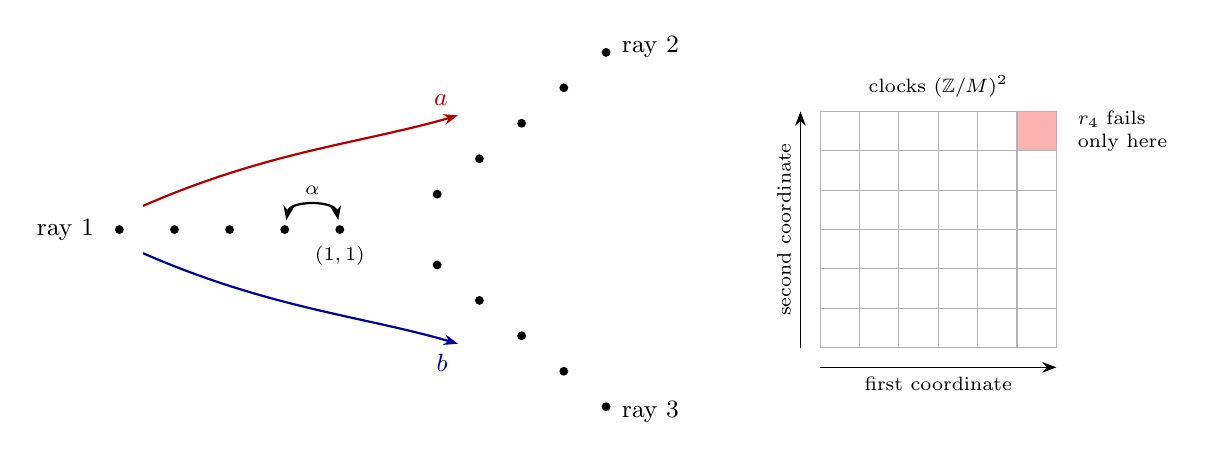
\begin{tikzpicture}[font=\small,>={Stealth[length=1.8mm]}]
\foreach \j in {1,...,5} {\fill ({-0.7*\j},0) circle (1.6pt);}
\foreach \j in {1,...,5} {\fill ({0.7*\j*cos(40)},{0.7*\j*sin(40)}) circle (1.6pt);}
\foreach \j in {1,...,5} {\fill ({0.7*\j*cos(40)},{-0.7*\j*sin(40)}) circle (1.6pt);}
\node[left] at (-3.7,0) {ray 1};
\node[right] at ({3.6*cos(40)},{3.6*sin(40)}) {ray 2};
\node[right] at ({3.6*cos(40)},{-3.6*sin(40)}) {ray 3};
\node[below=1pt] at (-0.7,-0.05) {\scriptsize$(1,1)$};
\draw[->,thick,red!70!black] (-3.2,0.3) .. controls (-1.6,1.0) and (-0.4,1.1) .. (0.8,1.45) node[above left]{$a$};
\draw[->,thick,blue!60!black] (-3.2,-0.3) .. controls (-1.6,-1.0) and (-0.4,-1.1) .. (0.8,-1.45) node[below left]{$b$};
\draw[<->,thick] (-0.72,0.12) to[bend right=80] node[above]{\scriptsize$\alpha$} (-1.38,0.12);
\begin{scope}[xshift=5.4cm,yshift=-1.5cm]
\fill[red!30] (2.5,2.5) rectangle (3,3);
\draw[step=0.5,gray!60] (0,0) grid (3,3);
\node[above] at (1.5,3.05) {\scriptsize clocks $(\mathbb Z/M)^2$};
\node[anchor=west,align=left,font=\scriptsize] at (3.15,2.75) {$r_4$ fails\\only here};
\draw[->] (0,-0.25) -- (3,-0.25) node[midway,below]{\scriptsize first coordinate};
\draw[->] (-0.25,0) -- (-0.25,3) node[midway,above,sloped]{\scriptsize second coordinate};
\end{scope}
\end{tikzpicture}
\caption{Left: Houghton's group $H_3$ acts on three rays of points. The generator $a$ translates along rays 1 and 2: points of ray 1
move toward the centre and on into ray 2. The generator $b$ does the same with rays 1 and 3, and $\alpha$ swaps the first two points of
ray 1. Right: a corner model (Section~\ref{sec:corner}) follows the quotient $\mathbb Z^2$ on a clock torus $(\mathbb Z/M)^2$ and colours
the points. The relation $r_4=aba^{-1}b^{-1}\alpha^{-1}$ fails only over one corner clock, a fraction $M^{-2}$ of the model, whose
size is $\exp(O(M))$.}
\label{fig:houghton}
\end{figure}

\paragraph{The group.} Let $Y=\{(i,j):i\in\{1,2,3\},\,j\ge1\}$ be three rays. Permutations act on the right and
$gh$ means $g$ followed by $h$. Let $a$ send $(1,1)\mapsto(2,1)$, $(1,j)\mapsto(1,j-1)$ for $j\ge2$ and
$(2,j)\mapsto(2,j+1)$, fixing ray~3; let $b$ be defined in the same way with rays 2 and 3 exchanged; let $\alpha$ be
the transposition of $(1,1)$ and $(1,2)$. These generate $H_3$, the group of permutations of $Y$ that are eventually
translations on each ray. They satisfy
\begin{equation}\label{eq:relators}
r_1=\alpha^2,\quad r_2=(\alpha a\alpha a^{-1})^3,\quad r_3=[\alpha,a^2\alpha a^{-2}],\quad
r_4=aba^{-1}b^{-1}\alpha^{-1},\quad r_5=a\alpha a^{-1}b\alpha^{-1}b^{-1},
\end{equation}
with $[x,y]=xyx^{-1}y^{-1}$; each identity can be checked directly on the finitely many points where the word
moves anything. By a theorem of Johnson (see~\cite[Theorem~2.8]{Lee2012}) these relators present $H_3$. The lower
bound below uses only that $r_1,\dots,r_5$ hold in $H_3$, the far-commutator areas of Section~\ref{sec:imported}, and
that the three-cycle $\gamma=\alpha\,(a\alpha a^{-1})$ on $(1,1),(1,2),(1,3)$ is nontrivial. The short exact sequence
$1\to\FSym(\mathbb{N})\to H_3\to\mathbb{Z}^2\to1$ shows that $H_3$ is elementary amenable.

\paragraph{The channel.} Introduce formal symbols for the six letters $a^{\pm1},b^{\pm1},\alpha^{\pm1}$ and for every
proper prefix of length at least two of each relator; there are 33 symbols. Each relator of length $l$ contributes
$l-1$ multiplication triangles $(x,y,z)$ meaning $xy=z$ along its prefixes, and three further triangles record
$ss^{-1}=e$ for $s\in\{a,b,\alpha\}$; there are 35 triangles. For unitaries $\lambda(w)$ assigned to the symbols,
set
\[
U_\lambda=\diag\big(1,(\lambda(w))_{w}\big)\ \oplus\ \bigoplus_{(x,y,z)}\frac{1}{\sqrt2}
\begin{pmatrix}1&\lambda(y)\\ \lambda(x)&-\lambda(x)\lambda(y)\end{pmatrix},
\]
an operator on $\mathbb{C}^{104}\otimes\mathcal{H}$ ($104=1+33+2\cdot35$). Each block is unitary for arbitrary
unitaries $\lambda(x),\lambda(y)$, so $U_\lambda$ is unitary. The channel $\Phi_H$ is defined with $\lambda$ the right
regular representation of $H_3$ and the bath in the canonical trace of the group von Neumann algebra:
$\Phi_H(\rho)=(\mathrm{id}\otimes\tau)[U_\lambda(\rho\otimes1)U_\lambda^*]$. Because the relators hold, the lower right
entry $-\lambda(x)\lambda(y)$ of each triangle block equals $-\lambda(z)$.

\begin{proposition}[Finite approximants]\label{prop:upper-profile}
For every $M\ge1$ there is a finite tracial factorization of bath dimension $M^2(2M)!$ whose channel is within
$\dJ$-distance $\min(1,26/M)$ of $\Phi_H$. Hence $\log\DChoi_{\Phi_H}(\delta)\le(55/\delta)\log(54/\delta)$ for
$0<\delta\le1/2$.
\end{proposition}

\begin{proof}
Let $\Omega=\{(1,j):1\le j\le2M\}$ and $F_M=\{\sigma a^m b^{n}:\ \sigma\in\Sym(\Omega),\ 0\le m,n<M\}$. The
translation part determines $(m,n)$ and then $\sigma$, so $|F_M|=M^2(2M)!$. With $t(p)=a^mb^n$ and the cocycle
$c(p,s)=t(p)\,s\,t(p+\pi(s))^{-1}$ one computes $c(p,b)=e$, $c(p,a)=a^m\varsigma_na^{-m}$ with
$\varsigma_n=b^nab^{-n}a^{-1}$ the cycle $(1,1)\to(1,2)\to\cdots\to(1,n+1)\to(1,1)$, and $c(p,\alpha)$ the transposition
of $(1,m+n+1)$ and $(1,m+n+2)$. All lie in $\Sym(\Omega)$ when the translation coordinates stay in $[0,M)^2$. Hence
$F_M\alpha=F_M$, and each of $a^{\pm1},b^{\pm1}$ moves exactly a fraction $1/M$ of $F_M$ out of $F_M$. Extend the
partial bijections $x\mapsto xs^{-1}$ inside $F_M$ to permutations $P_s$ of $F_M$ and use them as $\lambda(s)$; for a
prefix symbol use the product of the corresponding $P_s$. No relation is imposed on the $P_s$, and $U_P$ is unitary by
construction.

The normalized Choi state of the finite channel is the average over $x\in F_M$ of states $\mathcal{J}_x$, each the
(normalized) Gram matrix of the entry vectors at $x$. Call $x$ good if every entry word, read letter by letter from
$x$, stays inside $F_M$; then the entry vectors at $x$ are distinct basis vectors exactly when the words are distinct
in $H_3$, so $\mathcal{J}_x=\mathcal{J}(\Phi_H)$. The five relator paths contain $0,6,8,4,4$ translation letters and the
four single-letter symbols add four more; each translation step expels at most a fraction $1/M$ of the surviving
points, because the preceding partial word map is injective. So at most a fraction $26/M$ of points is bad, and
$\mathcal{J}(\Phi_M)=(1-t)\mathcal{J}(\Phi_H)+t\mathcal{J}_{\rm bad}$ with $t\le\min(1,26/M)$. Choosing
$M=\lceil26/\delta\rceil\le27/\delta$ and $\log(M^2(2M)!)\le(2M+2)\log(2M)$ gives the bound.
\end{proof}


\begin{proposition}[Choi rank and entropy]\label{prop:entropy-H}
The entries of $U_\lambda$ carry exactly $26$ distinct elements of $H_3$. Grouping entries by element,
$U_\lambda=\sum_{g\in\mathcal G}K_g\otimes\lambda(g)$ with $|\mathcal G|=26$ and $K_g\in M_{104}$ of pairwise disjoint supports, so
\[
\Phi_H(\rho)=\sum_{g\in\mathcal G}K_g\rho K_g^*,\qquad
\mathcal J(\Phi_H)=\frac1d\sum_{g\in\mathcal G}|K_g\rangle\!\rangle\langle\!\langle K_g|,
\]
the Choi rank of $\Phi_H$ is $26$, and $H(\Phi_H)=\log26$.
\end{proposition}

\begin{proof}
The entry labels are the identity, the $33$ symbols, and the lower-right entries of the triangles, which equal
$-\lambda(x)\lambda(y)=-\lambda(z)$ and whose elements are therefore among the symbols or the identity. Evaluating the $34$ labels as permutations of the rays
shows exactly $26$ distinct elements, listed in Table~\ref{tab:labels}. Writing $p_{i,l}$ for the prefix of length $l$ of $r_i$,
the eight coincidences are $p_{2,2}=p_{3,2}$ (the same word $\alpha a$) and seven consequences of the relators:
$p_{2,11}=p_{3,11}=a$, $p_{5,5}=b$, $\alpha^{-1}=p_{4,4}=\alpha$, $p_{2,9}=p_{5,3}=a\alpha a^{-1}$ and $p_{2,10}=p_{5,2}=a\alpha$. Every
label is $h\,a^ub^v$ with $(u,v)=\pi(g)$ and $h$ a permutation of the points $(1,1),\dots,(1,4)$, and labels with the same
translation have different $h$. Disjoint supports make the $K_g$ orthogonal, hence linearly
independent, and $\tau(\lambda(g)\lambda(h)^*)=\delta_{gh}$ gives the displayed formulas. Every $g$ has a singleton
diagonal position $i_g$ whose column contains only the entry of $K_g$. For $\rho=\frac1{26}\sum_g|i_g\rangle\langle i_g|$
the complementary output
\[
\Phi_H^c(\rho)_{gh}=\mathrm{Tr}(K_g\rho K_h^*)=\delta_{gh}/26
\]
is maximally mixed, and $\log26$ is the largest entropy of a complement of dimension $26$.
\end{proof}

\begin{table}[t]
\centering
\small
\begin{tabular}{@{}lp{12.2cm}@{}}
\toprule
$\pi(g)$ & labels $g=h\,a^ub^v$ and their permutations $h$ of the points $(1,1),\dots,(1,4)$, written $1,\dots,4$\\
\midrule
$(0,0)$ & $e$: $\mathrm{id}$;\ \ $\alpha=\alpha^{-1}=p_{4,4}$: $(1\,2)$;\ \ $p_{2,4}$: $(1\,3\,2)$;\ \ $p_{2,5}$: $(1\,3)$;\ \ $p_{2,8}$: $(1\,2\,3)$;\ \
$p_{2,9}=p_{5,3}$: $(2\,3)$;\ \ $p_{3,6}$: $(1\,2)(3\,4)$;\ \ $p_{3,7}$: $(3\,4)$\\
$(1,0)$ & $a=p_{2,11}=p_{3,11}$: $\mathrm{id}$;\ \ $p_{2,2}=p_{3,2}$: $(1\,2)$;\ \ $p_{2,3}$: $(1\,3\,2)$;\ \ $p_{2,6}$: $(1\,3)$;\ \
$p_{2,7}$: $(1\,2\,3)$;\ \ $p_{2,10}=p_{5,2}$: $(2\,3)$;\ \ $p_{3,5}$: $(1\,2)(3\,4)$;\ \ $p_{3,8}$: $(3\,4)$\\
$(2,0)$ & $p_{3,3}$: $(1\,2)$;\ \ $p_{3,4}$: $(1\,2)(3\,4)$;\ \ $p_{3,9}$: $(3\,4)$;\ \ $p_{3,10}$: $\mathrm{id}$\\
$(0,1)$ & $b=p_{5,5}$: $\mathrm{id}$;\ \ $p_{4,3}$: $(1\,2)$;\ \ $p_{5,4}$: $(2\,3)$\\
$(1,1)$ & $p_{4,2}$: $\mathrm{id}$\\
$(-1,0)$, $(0,-1)$ & $a^{-1}$: $\mathrm{id}$;\ \ $b^{-1}$: $\mathrm{id}$\\
\bottomrule
\end{tabular}
\caption{The $26$ elements of $H_3$ carried by the entries of $U_\lambda$, grouped by translation. Here $p_{i,l}$ is the prefix of length
$l$ of $r_i$, a permutation is written in cycle notation, and $g=h\,a^ub^v$ means $h$ followed by $a^ub^v$.}
\label{tab:labels}
\end{table}

\subsection{A symmetry of $H_3$ and exact translations in a box}\label{sec:symmetry}

Let $\pi:H_3\to\mathbb Z^2$ be the quotient map with $\pi(a)=(1,0)$, $\pi(b)=(0,1)$, $\pi(\alpha)=0$. An element $g$ with
$\pi(g)=(u,v)$ is eventually a translation by $(-u-v,u,v)$ on the three rays.

Let $\theta$ be the automorphism of $H_3$ given by conjugation with the relabelling $1\to2\to3\to1$ of the rays. A direct
check on the rays gives
\begin{equation}\label{eq:theta}
\begin{array}{c|ccc}
 &a&b&\alpha\\ \hline
\theta&a^{-1}b&a^{-1}&a^{-2}\alpha a^2\\
\theta^2&b^{-1}&b^{-1}a&b^{-2}\alpha b^2
\end{array}
\end{equation}
and $\theta^3=\mathrm{id}$. Since $\theta$ permutes the translation vector $(-u-v,u,v)$ cyclically, and its entries sum to zero,
\begin{equation}\label{eq:drift}
\sum_{j=0}^{2}\pi\big(\theta^j(g)\big)=0\qquad(g\in H_3).
\end{equation}
Every entry label of $U_\lambda$ has a word of length at most $12$, each $\theta^j$ multiplies word length by at most $5$
by~\eqref{eq:theta}, and $\|\pi(\theta^j(g))\|_\infty\le2$ for every label: $\pi(\theta(g))=(-u-v,u)$ and
$\pi(\theta^2(g))=(v,-u-v)$ when $\pi(g)=(u,v)$, and Table~\ref{tab:labels} lists the possible $\pi(g)$. The $\theta$-twisted unitaries
\[
U_j^\infty=\sum_{g\in\mathcal G}K_g\otimes\lambda(\theta^j(g)),\qquad j=0,1,2,
\]
arise from the same block construction with labels $\lambda(\theta^j(w))$; their lower-right entries are
$-\lambda(\theta^j(x))\lambda(\theta^j(y))=-\lambda(\theta^j(z))$, and their tracial channel is $\Phi_H$ because $\theta^j$ is injective.

\begin{lemma}[Exact translations in the box]\label{lem:box}
Let $F_M$ be as in the proof of Proposition~\ref{prop:upper-profile}. If $f\in F_M$, $s\in\{a^{\pm1},b^{\pm1},\alpha^{\pm1}\}$
and both $\pi(f)$ and $\pi(fs)$ lie in $[0,M)^2$, then $fs\in F_M$. Consequently a word of length $L$ is evaluated
exactly, letter by letter inside $F_M$, from every $f$ whose quotient position has distance at least $L$ from the boundary of
the box.
\end{lemma}

\begin{proof}
Write $f=\sigma\,t(p)$ with $t(p)=a^ub^v$. For a positive letter, $fs=\sigma\,c(p,s)\,t(p+\pi(s))$, and the cocycles
$c(p,a)=a^u\varsigma_va^{-u}$, $c(p,b)=e$ and $c(p,\alpha)$ are permutations of $(1,1),\dots,(1,u+v+2)$, which lie in
$\Omega$ when both positions are in the box. For an inverse letter, $t(p)s^{-1}=c(p-\pi(s),s)^{-1}\,t(p-\pi(s))$. The
property was also checked by machine for $M=2,3$.
\end{proof}

The support profile asks only for constant diamond accuracy, and a coarser register suffices for it.

\begin{proposition}[Coloring approximants]\label{prop:coloring}
Let $0<v\le2^{-17}$, $M=\lceil104/v\rceil$ and $q=2^{20}$. There is a finite tracial factorization of bath dimension at most
$M^2q^{2M}$ whose channel is within half-diamond distance $1/8$ of $\Phi_H$ and has support leakage at most $v$. Hence
$\log\Dsupp_{\Phi_H}(1/8,v)\le40M+2\log M$.
\end{proposition}

\begin{proof}
Split the $2M$ points of $\Omega$ into $q$ classes of sizes $k_1,\dots,k_q$ differing by at most one, let $G$ be the product of the
symmetric groups of the classes, and let the bath basis be the set $G\backslash F_M$ of cosets $Gx$, $x\in F_M$; it has
$M^2(2M)!/\prod_jk_j!\le M^2q^{2M}$ elements. Left multiplication by $G$ commutes with right multiplication, so the partial
bijections $x\mapsto xs^{-1}$ of Proposition~\ref{prop:upper-profile} descend to partial bijections of the cosets. Extend them to
permutations, use them and their products for the prefix symbols in place of $\lambda$, and keep the bath flat. Every entry of
$U_\lambda$ carries a word of length at most $12$, so the entries $a,b$ of the gadget satisfy $R_aR_b^*=R_w$ for a word $w$ of
length at most $24$. Call a coset good if its clock position has distance at least $24$ from the boundary of the box; the bad
fraction is $\beta\le96/M\le v$. By Lemma~\ref{lem:box}, every word of length at most $24$ acts on good cosets through right
multiplication by the element of $H_3$ it represents.

\emph{Accuracy.} If $w$ represents $1$, then $|\tau(R_w)-1|\le\beta$. If $w$ represents an element $g\ne1$ and moves the clock
position, it fixes no good coset. Otherwise $g$ acts on a good coset $G\sigma t(p)$ as $\sigma\mapsto\sigma c$ for a
nonidentity permutation $c$ of $\Omega$, and fixes the coset only if $\sigma c\sigma^{-1}\in G$, which requires two points of a
nontrivial cycle of $c$ to lie in the same class after applying $\sigma$. For a uniformly distributed coset at a fixed clock
this has probability at most $\sum_jk_j(k_j-1)/(2M(2M-1))\le2/q$. Hence $|\tau(R_w)|\le\beta+2/q$. The normalized Choi state is
$\frac1d\sum_{a,b}c_a\bar c_b\,\tau(R_aR_b^*)\,|r_as_a\rangle\langle r_bs_b|$ over the $174$ nonzero entries $c_a|r_a\rangle\langle s_a|$ of
the gadget, whose coefficients satisfy $\sum_a|c_a|^2=d=104$, while that of $\Phi_H$ has $\delta_{g_ag_b}$ in place of the traces.
The trace-norm difference is therefore at most $\frac1d(\sum_a|c_a|)^2(\beta+2/q)\le174(\beta+2/q)$, and by~\eqref{eq:dJ-ddia}
the half-diamond distance is at most $9048(\beta+2/q)\le9048(2^{-17}+2^{-19})<1/8$.

\emph{Leakage.} The flat bath is the uniform mixture of the basis cosets. For a good coset $x$, the Kraus operators with bath
input $x$ are $\sum_g[y=xg^{-1}]K_g$ for the matrices $K_g$ of Proposition~\ref{prop:entropy-H}, because entries carrying the same
element of $H_3$ act identically on $x$; so the Choi state of that input lies in the support of $\mathcal J(\Phi_H)$. The leakage is
at most $\beta\le v$.
\end{proof}

At fixed $q$ this construction does not approach $\Phi_H$ in Choi distance, so the Choi profile keeps the bound of
Proposition~\ref{prop:upper-profile}.

\subsection{What we use from the group paper}\label{sec:imported}

The lower bounds use the following results about approximate representations of Johnson's presentation, proved in the companion
paper~\cite{DouglasMghirbiA}; we state them here without proof. Let $P=\langle a,b,\alpha\mid r_1,\dots,r_5\rangle$, put
$\sigma_j=a^j\alpha a^{-j}$, and let $A^*(M)$ be the largest area in $P$ of a commutator $[\sigma_p^{\pm1},\sigma_q^{\pm1}]$ with
$0\le p,q\le M$ and $|p-q|\ge2$. These commutators are trivial in $H_3$ because the transpositions have disjoint supports.

\begin{theorem}[Reweighted far-commutator area]\label{thm:area-weighted}
$A^*(M)\le135\,M^{\log107}$ for every $M\ge2$.
\end{theorem}

\begin{proposition}[Quadratic lower bound]\label{prop:area-lower}
For odd $k\ge9$, $\mathrm{Area}(C_k)\ge(k-7)(k-5)/8$, where $C_k=[\alpha,a^k\alpha a^{-k}]$. Hence $A^*(R)\ge R^2/16$ for every integer $R\ge23$.
\end{proposition}

The area bound is proved by a doubling self-similarity of $H_3$, with finite relations certified by machine;
\cite{DouglasMghirbiA} also gives the certified bound $A^*(M)\le M^{11}$. Write $\mathrm{k}(u,v)=\|uv-vu\|_2$ and
$G(t)=h_2(\min\{\frac23t,\frac23\})+\min\{\frac23t,\frac23\}$.

\begin{lemma}[Projection products]\label{lem:projections}
Let $P_1,\dots,P_m$ be orthogonal projections on a Hilbert space and $\|x\|=1$. Then
$1-\mathrm{Re}\langle x,P_m\cdots P_1x\rangle\le2\sum_j\|(I-P_j)x\|^2$.
\end{lemma}

\begin{lemma}[Exact $S_3$ rounding]\label{lem:s3round}
If $A,B\in U(D)$ satisfy $\|A^2-I\|_2,\|B^2-I\|_2,\|(AB)^3-I\|_2\le e$, there is a unitary representation $u$ of
$S_3=\langle s,t\mid s^2,t^2,(st)^3\rangle$ on $\mathbb C^D$ with $\|u(s)-A\|_2\le e$, $\|u(t)-B\|_2\le8e$ and $\|u(st)-AB\|_2\le9e$, and
each normal form $1,s,t,st,ts,sts$ evaluated in $u$ is within $10e$ of the same word in $A,B$.
\end{lemma}

\begin{theorem}[Phase-robust sector bound]\label{thm:phase-robust}
Let $c_i,x_i\in U(D)$, $1\le i\le N$, satisfy $c_i^3=x_i^2=I$ and $x_ic_ix_i=c_i^{-1}$, with no condition on the commutators of
$x_i$ and $x_j$. Put $\Delta_i=\|c_i-I\|_2$ and $f(g)=c_1^{g_1}\cdots c_N^{g_N}$ for $g\in\mathbb Z_3^N$, let $g^{(i)}$ be $g$ with its
$i$-th coordinate negated, and, for uniform $g$,
\[
\hat a_i^2=\mathbb E_g\|f(g+e_i)-f(g)c_i\|_2^2,\qquad \hat b_i^2=\mathbb E_g\|x_if(g^{(i)})-f(g)x_i\|_2^2 .
\]
Then $\hat a_i^2\le\frac43\sum_{j>i}\mathrm{k}(c_i,c_j)^2$, $\hat b_i^2\le\frac43\sum_{j\ne i}\mathrm{k}(x_i,c_j)^2$, and
\[
\log D\ \ge\ \sum_{i=1}^N\Big[\frac{(\Delta_i^2-\hat a_i^2)_+}3-\frac{\hat b_i^2}{2\ln2}-G(\hat a_i^2)\Big].
\]
In particular $\Delta_i\ge49/100$ and $\hat a_i,\hat b_i\le1/100$ for all $i$ give $\log D\ge N/16$.
\end{theorem}

Call $\phi:\{a,b,\alpha\}\to U(D)$ an $e$-representation if $\|\phi(r_i)-I\|_2\le e$ for $i=1,\dots,5$, where $\phi$ is extended to the
free group. If $w$ is null in $P$ with area $A$, then $\|\phi(w)-I\|_2\le Ae$.

\begin{proposition}\label{prop:dimension}
Let $\phi$ be an $e$-representation with $\|\phi(\gamma)-I\|_2\ge1/2$, and let $N\ge1$ satisfy $750\sqrt N\,A_Ne\le1$, where
$A_N=\max\{1,A^*(3N)\}$. Then $\log D\ge N/16$.
\end{proposition}

\subsection{Corner models}\label{sec:corner}

The approximants above fail on a layer of about $M$ clock positions out of $M^2$. A torus of clock positions with a single bad
corner does better. Fix integers $M\ge2$ and $s\ge2$, put $\ell=2M+2$ and $L=3\ell$, and let $\Omega_{M,s}=(\mathbb Z/M\mathbb Z)^2\times[s]^L$.
For $2\le r\le L$ let $c_r=(1\ r\ r{-}1\ \cdots\ 2)\in\Sym(L)$ be the reverse cycle and $\tau=(1\ 2)$; products of permutations are read
from left to right, and a permutation $\pi$ of the coordinates acts on colorings by $(x\cdot\pi)(t)=x(t\pi^{-1})$. For $0\le i,j<M$ put
$A_{i,j}=c_{\ell-i-j}$ and, for $j<M-1$, $B_{i,j}=c_{2\ell-j}$. On the top row put $B_{i,M-1}=D_i$, where
\begin{equation}\label{eq:corner-rec}
D_0=c_{2\ell-M+1},\qquad D_{i+1}=c_{\ell-i-(M-1)}^{-1}\,\tau\,D_i\,c_{\ell-i}\qquad(0\le i<M-1).
\end{equation}
Define permutations of $\Omega_{M,s}$, with clock coordinates modulo $M$, by
\[
(i,j,x)\cdot a=(i+1,j,x\cdot A_{i,j}),\qquad(i,j,x)\cdot b=(i,j+1,x\cdot B_{i,j}),\qquad(i,j,x)\cdot\alpha=(i,j,x\cdot\tau).
\]

\begin{proposition}[Corner models~{\cite{DouglasMghirbiA}}]\label{prop:corner}
In these permutations $r_1,r_2,r_3,r_5$ hold exactly and $r_4$ fails only at the clock $(M-1,M-1)$, where it acts as the product
$R_M=(1\ \,M{+}4)\prod_{t=5}^{M+3}(t\ \,t{+}M)$ of $M$ disjoint transpositions of the colours; so every relator moves at most
a fraction $M^{-2}$ of $\Omega_{M,s}$, and $\gamma$ moves a fraction $1-s^{-2}$. At every clock the colour permutations of
$a\alpha a^{-1}$, $a^2\alpha a^{-2}$ and $b\alpha b^{-1}$ are $(2\ 3)$, $(3\ 4)$ and $(2\ 3)$. A word of length at most $t$ that represents a nonidentity
element of $H_3$ fixes at most a fraction $s^{-1}+4t/M$ of $\Omega_{M,s}$ when $M>2t$.
\end{proposition}

The proof is in~\cite{DouglasMghirbiA}; it also records the identities $c_r\tau c_r^{-1}=(2\ 3)$ and $c_r(2\ 3)c_r^{-1}=(3\ 4)$ for $r\ge4$
used below.

\begin{proposition}[Corner channels]\label{prop:corner-channel}
For $s=2^{20}$ and $M\ge2^{24}$ the gadget built from these permutations is a finite tracial factorization of bath dimension
$M^2s^{6M+6}$ within half-diamond distance $1/16$ of $\Phi_H$, with support leakage at most $M^{-2}$. Hence, for every $v>0$,
\[
\log\Dsupp_{\Phi_H}(1/8,v)\le120M+120+2\log M,\qquad M=\max\{2^{24},\lceil v^{-1/2}\rceil\}.
\]
\end{proposition}

\begin{proof}
Put $P(g)|\omega\rangle=|\omega g^{-1}\rangle$ and use these permutation unitaries in the gadget of
Section~\ref{sec:houghton}; every block stays unitary, so this is a finite tracial factorization of bath dimension $M^2s^{6M+6}$. Two
literal entry words that carry the same element of $H_3$ are related by one relator: the full relators equal $e$, and the other
coincidences are $p_{2,11}=p_{3,11}=a$, $p_{5,5}=b$, $\alpha^{-1}=p_{4,4}=\alpha$, $p_{2,9}=a\alpha a^{-1}$ and $p_{2,10}=a\alpha$, where
$p_{i,l}$ is the prefix of length $l$ of $r_i$ (for instance $p_{2,11}a^{-1}=r_2$ and $p_{4,4}\alpha^{-1}=r_4$ freely). Since
$r_1,r_2,r_3,r_5$ are exact, only the identifications through $r_4$ can fail, on at most a fraction $M^{-2}$ of the states; so
$1-\tau(P(w_\nu)^*P(w_\mu))\le M^{-2}$ whenever two entry words $w_\mu,w_\nu$ carry the same element. Write the entries of the gadget as
$c_\mu P(w_\mu)$, put $a_\mu=|c_\mu|^2/104$ and $p_g=\sum_{w_\mu=g}a_\mu$. The support projection of $\mathcal J(\Phi_H)$ is
$\sum_gv_gv_g^*/p_g$ with $v_g=104^{-1/2}\sum_{w_\mu=g}c_\mu|\mu\rangle$, and a direct computation gives the leakage of the resulting channel $\Psi$
\[
\ell_{\Phi_H}(\Psi)=\sum_g\frac1{p_g}\sum_{w_\mu=w_\nu=g}a_\mu a_\nu\big[1-\tau(P(w_\nu)^*P(w_\mu))\big]\le M^{-2}\sum_gp_g=M^{-2}.
\]
For entries carrying different elements the comparison word has length at most $24$, so its normalized trace is at most
$\eta=s^{-1}+96/M$; for equal elements the error is at most $M^{-2}\le\eta$. As in the proof of Proposition~\ref{prop:coloring} the
half-diamond distance is at most $9048\eta$, which for $s=2^{20}$ and $M\ge2^{24}$ is at most $9048\cdot112\cdot2^{-24}<1/16$. The bath
dimension has $\log(M^2s^{6M+6})=120M+120+2\log M$, and for $v>0$ the choice $M=\max\{2^{24},\lceil v^{-1/2}\rceil\}$ gives leakage at
most $v$.
\end{proof}

\begin{proposition}[Sharper corner models]\label{prop:corner-sharp}
Let $M\ge4$ and $s\ge2$, and drop the last $2M+2$ colour coordinates, which no generator moves. The gadget built from the resulting
permutations of $(\mathbb Z/M\mathbb Z)^2\times[s]^{4M+4}$ is a finite tracial factorization $\Psi_{M,s}$ with
\[
\ell_{\Phi_H}(\Psi_{M,s})=\varkappa_0\,\frac{1-s^{-M}}{M^2},\quad\varkappa_0=\frac{122}{2925},\qquad
\ddia(\Psi_{M,s},\Phi_H)\le\frac7{2s}+\frac2{M^2}.
\]
Consequently, for $0<\delta\le1/4$, $\log\DChoi_{\Phi_H}(\delta)\le2\log M+(4M+4)\log\lceil7/\delta\rceil$ with $M=\lceil2/\sqrt\delta\rceil$,
which is $O(\delta^{-1/2}\log(1/\delta))$; and $\log\Dsupp_{\Phi_H}(1/8,v)\le24M+24+2\log M$ with $M=\max\{6,\lceil(\varkappa_0/v)^{1/2}\rceil\}$.
\end{proposition}

\begin{proof}
\emph{Normal forms.} By Proposition~\ref{prop:corner}, at every clock $\alpha$, $a\alpha a^{-1}$, $a^2\alpha a^{-2}$ and
$b\alpha b^{-1}$ act on the colours as $s_0=(1\ 2)$, $s_1=(2\ 3)$, $s_2=(3\ 4)$ and $s_1$ without moving the clock, and $\alpha^{-1}$
acts as $\alpha$. In every literal entry word in the letters $a^{\pm1},\alpha^{\pm1}$, each $\alpha^{\pm1}$ occurs at running $a$-exponent
$0$, $1$ or $2$, so moving the powers of $a$ to the right writes the word, as a permutation of the bath, as $h\,a^u$ with
$h\in\langle s_0,s_1,s_2\rangle\cong S_4$. The other literal words are $b^{\pm1}$, $bb^{-1}$, $ab$, $a\alpha a^{-1}b=s_1b$,
$a\alpha a^{-1}b\alpha^{-1}=b$ and $r_5=1$, and the three words
\[
aba^{-1}=r_4\,\alpha b,\qquad aba^{-1}b^{-1}=r_4\,\alpha,\qquad aba^{-1}b^{-1}\alpha^{-1}=r_4
\]
(identities in the free group), where $r_4$ acts as $R_M$ at the clock $(M-1,M-1)$ and trivially elsewhere. The permutations $s_0,s_1,s_2$
are Coxeter generators of $S_4$, as are the transpositions $\alpha$, $a\alpha a^{-1}$, $a^2\alpha a^{-2}$ of $(1,1),\dots,(1,4)$ in $H_3$.
So, apart from these three words, two literal words carrying the same element of $H_3$ act identically on the bath, and two carrying
different elements with the same translation act as $h\,t$ and $h'\,t$ with $h\ne h'$ (Table~\ref{tab:labels}).

\emph{Two exceptional clocks.} An entry acts by $P(w)|\omega\rangle=|\omega w^{-1}\rangle$. For the three words above, $\omega w^{-1}$
differs from the value of the normal form only when the path of $w^{-1}$ meets $r_4^{-1}$ at the clock $(M-1,M-1)$: for the last two
words this happens when $\omega$ is at $(M-1,M-1)$, and for $aba^{-1}$, whose inverse first applies $b^{-1}$, when $\omega$ is at
$(M-1,0)$. At every other clock $c$ each entry acts as its normal form. Let $\tau_c$ be the uniform state on the colourings at $c$.
For entries with normal forms $h\,t$ and $h'\,t'$, $\tau_c(P(w')^*P(w))$ is $0$ if $t\ne t'$, because the two words end at different
clocks: the translations in Table~\ref{tab:labels} differ by vectors with coordinates at most $3$ and $2$ in absolute value, and
$M\ge4$. If $t=t'$, it is the fraction of colourings fixed by a permutation conjugate to $h^{-1}h'$, which is $s^{-\iota(h^{-1}h')}$, with
$\iota$ the number of moved points minus the number of nontrivial cycles. So at every clock outside the two exceptional ones the channel
is $\Phi_s(X)=\sum_{g,h}G_{gh}K_gXK_h^*$, where $G_{gg}=1$, $G_{gh}=s^{-\iota}\le1/s$ for distinct labels with the same translation, and
$G_{gh}=0$ otherwise. Each clock gives a channel, because the gadget is unitary for any assignment, so
$\Psi_{M,s}=(1-2/M^2)\Phi_s+(2/M^2)\Xi$ for a channel $\Xi$.

\emph{Distance.} The map $V_0=\sum_gK_g\otimes|g\rangle$ is an isometry, and for a Hermitian matrix $H$,
$\sum_{g,h}H_{gh}K_gXK_h^*=\mathrm{Tr}_2[(I\otimes H^{T})V_0XV_0^*]$. With a reference system, the trace norm of such a weighted partial
trace is at most $\|H\|_{\rm op}$ times that of its argument, so
\begin{equation}\label{eq:gram-diamond}
\Big\|X\mapsto\sum_{g,h}H_{gh}K_gXK_h^*\Big\|_\diamond\le\|H\|_{\rm op}.
\end{equation}
The matrix $G-I$ is symmetric, with nonnegative entries at most $1/s$ and at most seven of them in each row, since no translation class
has more than eight labels. So $\|G-I\|_{\rm op}\le7/s$, $\ddia(\Phi_s,\Phi_H)\le7/(2s)$, and
$\ddia(\Psi_{M,s},\Phi_H)\le7/(2s)+2/M^2$.

\emph{Leakage.} In the leakage formula of the proof of Proposition~\ref{prop:corner-channel}, only the classes of $e$ and $\alpha$ contain literal
words that act differently. In squared-coefficient weight the class of $e$ has $45/2$, of which $1/2$ is the entry
$aba^{-1}b^{-1}\alpha^{-1}$ (the last triangle of $r_4$); the class of $\alpha$ has $25/2$, of which $2$ belongs to $aba^{-1}b^{-1}$. The
word $aba^{-1}$ is alone in its class and causes no leakage. For each pair of one of these two words and a correctly acting word of its
class, $1-\tau(P^*P')$ is the fraction $(1-s^{-M})/M^2$ of states moved by $R_M$, and all other pairs contribute zero. Hence
\[
\ell_{\Phi_H}(\Psi_{M,s})=\frac1{104}\Big(\frac{2\cdot\frac12\cdot22}{45/2}+\frac{2\cdot2\cdot\frac{21}2}{25/2}\Big)\frac{1-s^{-M}}{M^2}
=\frac{122}{2925}\cdot\frac{1-s^{-M}}{M^2}.
\]

\emph{Profiles.} For $0<\delta\le1/4$ take $s=\lceil7/\delta\rceil$ and $M=\lceil2/\sqrt\delta\rceil\ge4$: the half-diamond distance is
at most $\delta/2+\delta/2$, so by~\eqref{eq:dJ-ddia} the Choi distance is at most $\delta$, with bath dimension $M^2s^{4M+4}$. For the
support profile take $s=64$ and $M\ge6$: then $7/128+2/M^2<1/8$ and the leakage is at most $\varkappa_0/M^2\le v$.
\end{proof}

\begin{corollary}[A service from the corner models]\label{cor:corner-service}
Let $0<\epsilon\le1/2$ and $\log(256n/\epsilon)<n$. There is a causal service of $\Phi_H$ with error $\epsilon$, exchange
$J\le nH(\Phi_H)/2$, $C=0$, $P\le\lceil\log(n+1)\rceil+1$ and memory $Q=O(\sqrt{n/\epsilon}\,\log(n/\epsilon))$.
\end{corollary}

\begin{proof}
Apply Theorem~\ref{thm:closure-upper} with exchange slack $0$, so that its buffer is $C_d(\sqrt{nx}+\log(n+1))$ with $x=\log(256n/\epsilon)$,
and with $m=\DChoi_{\Phi_H}(\epsilon/(8dn))$, $d=104$. By Proposition~\ref{prop:corner-sharp}, $\log m=O(\sqrt{n/\epsilon}\log(n/\epsilon))$.
\end{proof}

At fixed error this is the order of Theorem~\ref{thm:sublinear}, reached through the general compiler and the static profile
alone.

\subsection{Smoothed corner models}\label{sec:smoothed}

In a permutation model a relator that fails costs the fraction of points it moves. In a unitary model it costs a sum of squared
angles, so a single defect can be spread thin. Doing this for the corner models gives unitary approximants of $\Phi_H$ whose leakage
is of order $M^{-3}$, not $M^{-2}$, at the same size. Throughout, products are read from left to right, the left factor acting first,
as in Section~\ref{sec:corner}, and $e_1=(1,0)$, $e_2=(0,1)$.

\emph{One-particle models.} Use the reduced colour coordinates $1,\dots,L$ with $L=4M+4$, and read each link permutation $A_c$, $B_c$
and $\tau$ of Section~\ref{sec:corner} as a permutation matrix on $\mathbb C^L$. A one-particle model replaces some of these link matrices
by unitaries. For a word $w$ and a clock $c$ the holonomy $W_c(w)\in U(L)$ is the product of the link matrices along the path of $w$ from
$c$, with inverse matrices for inverse letters. For a two-element set $S=\{x,y\}$ let $Q_S$ be the projector onto
$(e_x-e_y)/\sqrt2$; then $\exp(i\pi Q_S)$ is the transposition $(x\ y)$, and $\exp(i\vartheta Q_S)$ is a phase rotation in the plane of $S$.

\emph{Fermionic quantization.} For $W\in U(L)$ let $\Lambda(W)$ act on the exterior algebra $\Lambda(\mathbb C^L)$, of dimension $2^L$,
by $v_1\wedge\cdots\wedge v_m\mapsto Wv_1\wedge\cdots\wedge Wv_m$. It is multiplicative on all of $U(L)$, and
$\mathrm{Tr}\,\Lambda(W)=\det(I+W)$, since in degree $m$ its eigenvalues are the products of $m$ eigenvalues of $W$. For $k\ge1$ put
$\Lambda_k=\Lambda^{\otimes k}$, so that $2^{-kL}\,\mathrm{Tr}\,\Lambda_k(W)=\det\big((I+W)/2\big)^k$. The quantized model has bath
$\mathcal H=\mathbb C^{M^2}\otimes\Lambda(\mathbb C^L)^{\otimes k}$ with its normalized trace $\tau$. A letter moves the clock $c$ to
$c+\pi(s)$ and applies $\Lambda_k$ of its link matrix at $c$, and $\rho(s)$ is the adjoint of this operator, as for $P(g)$ in
Proposition~\ref{prop:corner}, so $\rho$ is a representation of the free group on $a,b,\alpha$. A word whose translation is nonzero
modulo $M$ has $\tau(\rho(w))=0$, and a word that closes has
\[
\|\rho(w)-I\|_2^2=\mathbb E_c\Big[2-2\,\mathrm{Re}\det\big((I+W_c(w))/2\big)^k\Big],
\]
with $\mathbb E_c$ the average over clocks. For a three-cycle $\sigma$ of coordinates $\det((I+\sigma)/2)=\frac14$.

\begin{lemma}[Rotating the links]\label{lem:rotations}
In a corner model, replace every link $A_c$ by $U_cA_c$ and every link $B_c$ by $V_cB_c$, where $U_c$ commutes with $(2\ 3)$ and
$(3\ 4)$, and $V_c$ commutes with $(2\ 3)$. Then at every clock the holonomies of $\alpha$, $a\alpha a^{-1}$, $a^2\alpha a^{-2}$ and
$b\alpha b^{-1}$ are $(1\ 2)$, $(2\ 3)$, $(3\ 4)$ and $(2\ 3)$, so $r_1,r_2,r_3,r_5$ have identity holonomy everywhere and $\gamma$ acts
as a three-cycle.
\end{lemma}


A plaquette $q$ with base $v_0$ has the vertices $v_0$, $v_1=v_0+e_1$, $v_2=v_0+e_2$, $v_0+e_1+e_2$; its bottom and top edges are the
$a$-links at $v_0$ and $v_2$, and its left and right edges the $b$-links at $v_0$ and $v_1$. Its $r_4$ holonomy is
$W_q=A_{v_0}B_{v_1}A_{v_2}^{-1}B_{v_0}^{-1}\tau$. A \emph{region} consists of a set $R$ of plaquettes, a source $q_0\in R$, a sign
$s_R=\pm1$, and a two-element label $\mathrm{lab}(v)\subset\{1,\dots,L\}$ at every vertex of every plaquette of $R$. An edge is
\emph{interior} if it lies on two plaquettes of $R$.

\begin{lemma}[Spreading a defect]\label{lem:spreading}
Take a permutation model satisfying the local identities
$A_c\tau A_c^{-1}=(2\ 3)$, $A_c(2\ 3)A_c^{-1}=(3\ 4)$ and $B_c\tau B_c^{-1}=(2\ 3)$ of Lemma~\ref{lem:rotations} at every clock.
Suppose $W_q$ is the identity except at finitely many sources, where it is the
product of the transpositions given by the base labels of the regions with that source. Let finitely many regions satisfy:
\begin{enumerate}[label=(R\arabic*),itemsep=0pt]
\item for each region $R$, every edge of a plaquette $q\in R$ other than its own source $q_0(R)$, from $v$ to $w$, carries $\mathrm{lab}_R(v)$ onto $\mathrm{lab}_R(w)$ under its link permutation, even if $q$ is another region's source;
\item every base label avoids $\{1,2\}$, and the label at the initial vertex of every interior edge avoids $\{2,3,4\}$;
\item each region is connected through its interior edges, and the only interior edge of its source is the bottom edge;
\item labels of different regions are disjoint wherever both are defined; on an interior link carrying a region's rotation, its label is disjoint from any additional modification of that link.
\end{enumerate}
Here the link permutations belong to the base model, including preliminary exact moves. Boundary potentials vanish, so a region
requires no disjointness from an additional modification on a link where it carries no rotation.
Let $F_{R,q}$ be real numbers with $\sum_{q\in R}F_{R,q}=s_R\pi$ for each region. Then there are potentials $\varphi_R$ on the interior
edges of $R$ such that the model with $U_c=\prod_R\exp(i\varphi_R(\text{$a$-edge at }c)\,Q_{\mathrm{lab}_R(c)})$ and
$V_c=\prod_R\exp(i\varphi_R(\text{$b$-edge at }c)\,Q_{\mathrm{lab}_R(c)})$ still has $r_1,r_2,r_3,r_5$ exact, and its $r_4$ holonomy at
every plaquette $q$ is $\prod_{R\ni q}\exp(iF_{R,q}Q_{\mathrm{lab}_R(v_0)})$, with $v_0$ the base of $q$.
\end{lemma}

Lemmas~\ref{lem:rotations} and~\ref{lem:spreading} are proved in~\cite[Section~6.2]{DouglasMghirbiA}, where the same construction gives unitary models of
Johnson's presentation.

\begin{proposition}[Smoothed corner models]\label{prop:smoothed}
For every $M\ge48$ there is a finite tracial factorization with bath dimension $M^2\,2^{8M+8}$ whose channel is within half-diamond
distance $0.106$ of $\Phi_H$ and has support leakage at most $0.3\,M^{-3}$. Its bath is flat, so its entropy production is zero.
Consequently, for every $v>0$, with $M=\max\{48,\lceil(0.3/v)^{1/3}\rceil\}$,
\[
\log\Dsupp_{\Phi_H}(1/8,v)\le8M+8+2\log M\qquad\text{and}\qquad\log D^{\mathrm{ent}}_{\Phi_H}(1/8,v)\le8M+8+2\log M.
\]
\end{proposition}

\begin{proof}
\emph{The unitary model.} We recall the construction of~\cite[Section~6.2]{DouglasMghirbiA}. Let $c^*=(M-1,M-1)$, where the $r_4$ holonomy is $R_M$
(Proposition~\ref{prop:corner}). Replace $A_{c^*}$ by $\eta_1A_{c^*}$ and $B_{(0,M-2)}$ by $\eta_2B_{(0,M-2)}$, with $\eta_1=(1\ \,M{+}4)$ and
$\eta_2=(5\ \,M{+}5)$. Then $r_1,r_2,r_3,r_5$ stay exact, the $r_4$ holonomy at $c^*$ becomes $\prod_{t=5}^{M+3}(t\ \,t{+}M)$, at $(0,M-2)$ it becomes
$\eta_2$, and elsewhere it is the identity.

\emph{The regions.} For $5\le t\le M+3$ let $R_t$ have source $c^*$ and sign $(-1)^{t-5}$, and consist of $c^*$, the plaquettes $(M-1,j)$
with $1\le j\le M-2$, and the plaquettes $(i,j)$ with $0\le i\le M-3$, $0\le j\le M-2$ and $i+j\le t+M-8$; label the vertex $(i,j)$ by
$\{t+M-1-i-j,\ t+2M-1-j\}$ for $0\le i\le M-2$ and $(M-1,j)$ by $\{t+M-1-j,\ t+2M-1-j\}$. Let $T$ have source $(0,M-2)$ and sign
$(-1)^{M-1}$, and consist of $(0,M-2)$ and the plaquettes $(i,j)$ with $i,j\ge0$ and $i+j\le M-3$, with labels $\{M+3-i-j,\ 2M+3-j\}$.
The source labels are the defect pairs $\{t,t+M\}$ at $c^*$ and $\{5,M+5\}$ at $(0,M-2)$.

These regions satisfy (R1)--(R4)~\cite[Section~6.2]{DouglasMghirbiA}. Moreover $R_t\subset R_{t+1}$, and every region has at least
$m_M=(M-1)(M-2)/2+1$ plaquettes.

\emph{The defect.} Take $F_{R,q}=s_R\pi/|R|$ on each region and $k=2$. By Lemma~\ref{lem:spreading} the $r_4$ holonomy at $q$ is a product
of phase rotations by angles $F_{R,q}$ in disjoint planes, so $\det((I+W'_q)/2)=\prod_R(1+e^{iF_{R,q}})/2=e^{i\Theta_q}C_q$ with
$\Theta_q=\frac12\sum_RF_{R,q}$ and $C_q=\prod_R\cos(F_{R,q}/2)\in[0,1]$. Using $1-C^k\le k(1-C)$, $1-\prod_Rc_R\le\sum_R(1-c_R)$ and
$1-\cos x\le x^2/2$,
\[
2-2\,\mathrm{Re}\big(e^{ik\Theta_q}C_q^k\big)=2(1-C_q^k)+2C_q^k(1-\cos k\Theta_q)\le\frac k4\sum_RF_{R,q}^2+k^2\Theta_q^2 .
\]
Summed over the plaquettes, $\sum_q\sum_RF_{R,q}^2=\sum_R\pi^2/|R|\le M\pi^2/m_M$. The bulk regions containing $q$ are those with $t$
at least some $t_q$; their signs alternate and their magnitudes $\pi/|R_t|$ decrease, so they sum to at most $\pi/m_M$ in absolute value,
and $T$ adds at most $\pi/m_M$. Hence $|\Theta_q|\le\pi/m_M$, and averaging over the $M^2$ clocks,
\[
M^3e_4^2:=M^3\|\rho(r_4)-I\|_2^2\le\frac{\pi^2M^2}{2m_M}+\frac{4\pi^2M^3}{m_M^2}
\le\frac{\pi^2M^2}{(M-1)(M-2)}+\frac{16\pi^2M^3}{(M-1)^2(M-2)^2},
\]
which decreases in $M$ and is below $14.26$ at $M=48$. So $e_4^2\le14.26\,M^{-3}$ for $M\ge48$.

\emph{The channel.} Build the gadget from $\rho$ with $k=2$; its bath has dimension $M^2\,2^{2L}=M^2\,2^{8M+8}$. By
Lemma~\ref{lem:rotations} the normal forms in the proof of Proposition~\ref{prop:corner-sharp} hold for $\rho$: every literal entry word
$u$ carrying a label $g$ has $\rho(u)=\rho(\hat g)$, where $\hat g=h\,t$ is the normal form of $g$, except $aba^{-1}$, $aba^{-1}b^{-1}$ and
$aba^{-1}b^{-1}\alpha^{-1}$, for which $\|\rho(u)-\rho(\hat g)\|_2=e_4$. For labels $g,g'$ with normal forms $\hat g=h\,t$ and $\hat g'=h'\,t'$,
$G_{gg'}=\tau(\rho(\hat g')^*\rho(\hat g))$ is $0$ if $t\ne t'$; otherwise the holonomy is conjugate to $h'^{-1}h$, a permutation of the
coordinates $1,\dots,4$, so $G_{gg'}$ is $\det((I_4+h'^{-1}h)/2)^k$ up to conjugation: $1$ if $h=h'$, $4^{-k}$ for a three-cycle, and $0$
for every other element of $S_4$, each of which has the eigenvalue $-1$. By Table~\ref{tab:labels}, in each translation class of eight labels
the three-cycle relation splits by parity into two copies of the complete graph on four vertices minus one edge, whose largest eigenvalue is
$(1+\sqrt{17})/2$, and the other classes give smaller graphs. So $\|G-I\|_{\rm op}=4^{-k}(1+\sqrt{17})/2$.

Write $U_\rho=W+R$ with $W=\sum_gK_g\otimes\rho(\hat g)$. For operators $A,B$ on $\mathbb C^{104}\otimes\mathcal H$ put
$V_A\psi=(A\otimes I)(\psi\otimes\Omega)$, with $\Omega\in\mathcal H\otimes\mathcal H$ a purification of $\tau$; then
$X\mapsto(\mathrm{id}\otimes\tau)[A(X\otimes I)B^*]$ has diamond norm at most $\|V_A\|\,\|V_B\|$, and $\|V_A\|$ is at most its
Hilbert--Schmidt norm. The remainder $R$ lives on the entries carrying the three exceptional words, of squared-coefficient weight
$2+2+\frac12$, so $\|V_R\|^2\le\frac92e_4^2$, and $\|V_W\|\le1+\|V_R\|$ because $V_{U_\rho}$ is an isometry. The channel of $W$ is
$X\mapsto\sum_{g,g'}G_{gg'}K_gXK_{g'}^*$, within diamond norm $\|G-I\|_{\rm op}$ of $\Phi_H$ by~\eqref{eq:gram-diamond}. Therefore
\[
\ddia(\Psi,\Phi_H)\le\tfrac12\|G-I\|_{\rm op}+\|V_R\|(1+\|V_R\|)+\tfrac12\|V_R\|^2<0.0801+0.0247+0.0003<0.106
\]
for $M\ge48$, since $\|V_R\|^2\le\frac92\cdot14.26\cdot48^{-3}<5.81\cdot10^{-4}$. In the leakage formula of the proof of
Proposition~\ref{prop:corner-channel}, with $1-\mathrm{Re}\,\tau(\rho(u')^*\rho(u))=\frac12\|\rho(u)-\rho(u')\|_2^2$ in place of
$1-\tau(P^*P')$, only the pairs counted in the proof of Proposition~\ref{prop:corner-sharp} contribute, each with $\frac12e_4^2$. So the
leakage is $\frac{\varkappa_0}2e_4^2=\frac{61}{2925}e_4^2\le\frac{61}{2925}\cdot14.26\,M^{-3}<0.3\,M^{-3}$.

\emph{Profiles.} The bath is flat, so the round has entropy production zero, and the choice of $M$ makes the leakage at most $v$ and the
distance below $1/8$. The logarithm of the bath dimension is $8M+8+2\log M$.
\end{proof}

So the one-round profile of $\Phi_H$ at distance $1/8$ grows at most like $\exp(O(v^{-1/3}))$, and Theorem~\ref{thm:one-round} cannot hold with any
exponent above $1/3$ in place of $\beta_H$. Sequential extraction reads the profile at the stricter distance $\epsilon/(1-\epsilon)$, so the ceiling
has to hold at every fixed distance; it does, with the fermionic power chosen from the distance.

\begin{proposition}[One-round profile at every fixed distance]\label{prop:smoothed-u0}
For every $u_0>0$ there is $C(u_0)$ such that $\log D^{\mathrm{ent}}_{\Phi_H}(u_0,v)\le C(u_0)\,v^{-1/3}$ and
$\log\Dsupp_{\Phi_H}(u_0,v)\le C(u_0)\,v^{-1/3}$ for $0<v\le1$.
\end{proposition}

\begin{proof}
Run the construction of the proof of Proposition~\ref{prop:smoothed} with fermionic power $k$ and $M\ge6$. Its estimates hold for every $k$:
$\|G-I\|_{\rm op}=4^{-k}(1+\sqrt{17})/2$, $\|V_R\|^2\le\frac92e_4^2$, the leakage is $\frac{\varkappa_0}2e_4^2$, and the defect computation gives
$e_4^2\le\frac{k\pi^2}{4Mm_M}+\frac{k^2\pi^2}{m_M^2}\le\frac{k\pi^2}{M^3}+\frac{16k^2\pi^2}{M^4}$, since $m_M\ge M^2/4$. Choose $k$ with
$4^{-k}(1+\sqrt{17})/4\le u_0/2$, and then $M$ so large that $\|V_R\|(1+\|V_R\|)+\frac12\|V_R\|^2\le u_0/2$ and the leakage is at most $v$; this needs
$M$ of order $(k/v)^{1/3}$. The bath is flat, so the entropy production is zero, and its dimension is $M^2\,2^{k(4M+4)}$.
\end{proof}

A memory lower bound obtained solely from this two-parameter one-round profile, as in Theorem~\ref{thm:constant-lower}, therefore cannot
exceed order $(n/(B+\log n))^{1/3}$ at a fixed error. This does not exclude stronger arguments that use more information about the extracted
round, or several rounds; and $C(u_0)$ grows as $u_0\to0$. Our permutation models have no such smoothing: in them the
fraction of points moved by a relator adds up over a van Kampen diagram~\cite{DouglasMghirbiA}, and the corner models, with exponent $1/2$, are
the best permutation approximants we know. Whether better permutation models exist is open.

\subsection{The Choi profile}\label{sec:choi}

The proof of Proposition~\ref{prop:smoothed} bounds the distance to $\Phi_H$ through the remainder $V_R$, which is of first order in the defect
$e_4$; this suffices at constant diamond accuracy. In Choi distance the defect enters only at second order. Fix $k\ge1$ and an even $M\ge6$; the
construction of the proof of Proposition~\ref{prop:smoothed}, and Lemmas~\ref{lem:rotations} and~\ref{lem:spreading}, need only $M\ge6$. Let $\rho=\rho_{M,k}$
be the resulting representation with fermionic power $k$, $\Psi_{M,k}$ its gadget channel, of bath dimension $M^22^{k(4M+4)}$, and $z=\tau(\rho(r_4))$.
Matrix products below are written with later letters on the left. For words $u,v$,
\begin{equation}\label{eq:fermion-moment}
\tau\big(\rho(v)^*\rho(u)\big)=M^{-2}\sum_c\mathbf 1[\mathrm{end}_u(c)=\mathrm{end}_v(c)]\,\det\Big(\frac{I+W_c(v)W_c(u)^*}2\Big)^k,
\end{equation}
where $\mathrm{end}_u(c)$ is the clock at which the path of $u$ from $c$ ends: on the fibre over $c$ the operator acts by $\Lambda_k(W_c(v)W_c(u)^*)$ when
the ends agree. Index the Choi matrices by the $174$ entries of the gadget as in the proof of Proposition~\ref{prop:corner-channel}, and let
$\Gamma$, $\Gamma^c$ and $\Gamma^H$ be $104$ times the Choi matrices of $\Psi_{M,k}$, of the channel $\Theta_G:X\mapsto\sum_{g,g'}G_{gg'}K_gXK_{g'}^*$ of the
proof of Proposition~\ref{prop:smoothed}, and of $\Phi_H$. Let EXC be the seven entries that carry the words $aba^{-1}$, $aba^{-1}b^{-1}$ and
$aba^{-1}b^{-1}\alpha^{-1}$.

\begin{lemma}[Structure]\label{lem:choi-structure}
$\Gamma_{\mu\nu}=\Gamma^c_{\mu\nu}$ unless exactly one of $\mu,\nu$ lies in EXC. For $\mu\in\mathrm{EXC}$ and $\nu\notin\mathrm{EXC}$, $\Gamma_{\mu\nu}=z\,\Gamma^c_{\mu\nu}$ and
$\Gamma_{\nu\mu}=\bar z\,\Gamma^c_{\nu\mu}$.
\end{lemma}

\begin{proof}
\emph{Holonomies.} A non-exceptional entry word $u$ with normal form $\hat u=h\,t$ has $W_c(u)=W_c(t)P_h$ at every clock, where $P_h$ permutes the
coordinates $1,\dots,4$: by Lemma~\ref{lem:rotations} the conjugates $\alpha$, $a\alpha a^{-1}$, $a^2\alpha a^{-2}$ act as $(1\,2)$, $(2\,3)$, $(3\,4)$,
and for words containing $b$ the relator $r_5$ is exact. An exceptional word is $u=r_4\hat u$ in the free group (proof of
Proposition~\ref{prop:corner-sharp}), so $W_c(u)=W_c(\hat u)W'_c$ with $W'_c$ the $r_4$ holonomy at the plaquette with base $c$, and the ends agree.
By Lemma~\ref{lem:spreading} $W'_c$ is a product of rotations in planes whose coordinates are at least $5$, so $W'_c=I_4\oplus R_c$; put
$\zeta_c=\det((I+R_c)/2)$. Since $\rho(s)$ is the adjoint of the transport operator, $z=M^{-2}\sum_c\overline{\zeta_c}^{\,k}$.

\emph{Canonical entries.} For labels with normal forms $h\,t$ and $h'\,t'$ and $t\ne t'$, the ends differ at every clock, since $M\ge6$ exceeds the
translation differences, and both entries vanish. For $t=t'$, $W_c(\hat u')W_c(\hat u)^*$ is similar to $P_{h'h^{-1}}\oplus I$, and
$\det((I_4+P)/2)^k$ is $1$ for the identity, $4^{-k}$ for a three-cycle and $0$ otherwise; this is $\Gamma^c$.

\emph{Exceptional entries.} Let $\mu$ be exceptional and $\nu$ not. Then
$W_c(w_\nu)W_c(w_\mu)^*=W_c(\hat w_\nu)W_c'^{\,*}W_c(\hat w_\mu)^*$, which is similar to
\[
W_c(\hat w_\mu)^*W_c(\hat w_\nu)W_c'^{\,*}=(P\oplus I)(I_4\oplus R_c^*)=P\oplus R_c^*,
\]
whose determinant factorizes; by~\eqref{eq:fermion-moment} the entry is the canonical one times $M^{-2}\sum_c\overline{\zeta_c}^{\,k}$. If both are exceptional the factors $W'_c$ cancel. The transposed entries are complex
conjugates.
\end{proof}

\begin{lemma}[Second order]\label{lem:second-order}
For even $M\ge6$, with $m_M=(M-1)(M-2)/2+1$,
\[
|1-z|\ \le\ \frac{k\pi^2}{8Mm_M}+\frac{k^2\pi^2}{2m_M^2}.
\]
\end{lemma}

\begin{proof}
In the notation of the proof of Proposition~\ref{prop:smoothed}, $\zeta_q=e^{i\Theta_q}C_q$ with $\Theta_q=\frac12\sum_{R\ni q}F_{R,q}$ and
$C_q=\prod_{R\ni q}\cos(F_{R,q}/2)\in[0,1]$. The net flux vanishes for even $M$: $\sum_q2\Theta_q=\pi\sum_Rs_R$, the $M-1$ bulk signs $(-1)^{t-5}$ sum to $1$,
and $s_T=(-1)^{M-1}=-1$. Hence, since $|1-z|=|1-\bar z|$,
\[
|1-z|=\Big|M^{-2}\sum_q\big(1+ik\Theta_q-\zeta_q^k\big)\Big|\le M^{-2}\sum_q\Big[\frac{k^2\Theta_q^2}2+\frac k8\sum_{R\ni q}F_{R,q}^2\Big],
\]
by $|e^{ix}-1-ix|\le x^2/2$, $1-C^k\le k(1-C)$, $1-\prod_Rc_R\le\sum_R(1-c_R)$ and $1-\cos x\le x^2/2$. As in that proof $|\Theta_q|\le\pi/m_M$ and
$\sum_q\sum_RF_{R,q}^2\le M\pi^2/m_M$.
\end{proof}

For odd $M$ the net flux is $\pi$ and $z$ differs from $1$ at first order; this is why $M$ is even.

\begin{lemma}[Choi distance]\label{lem:choi-distance}
$\dJ(\Psi_{M,k},\Phi_H)\le\frac{41}{32}4^{-k}+\Upsilon_k|1-z|$, where $104\,\Upsilon_k=\sqrt{21/2}+2\sqrt{21/4}+\sqrt{11}+4^{-k}\big(2+2\sqrt2+\sqrt6+2\sqrt3\big)$.
\end{lemma}

\begin{proof}
We have $\dJ(\Psi_{M,k},\Phi_H)\le\frac1{208}\|\Gamma-\Gamma^c\|_1+\frac1{208}\|\Gamma^c-\Gamma^H\|_1$. The second term is at most
$\ddia(\Theta_G,\Phi_H)\le\frac12\|G-I\|_{\rm op}$ by~\eqref{eq:gram-diamond}, and $\frac12\|G-I\|_{\rm op}=4^{-k}(1+\sqrt{17})/4\le\frac{41}{32}4^{-k}$ (proof of Proposition~\ref{prop:smoothed}). By
Lemma~\ref{lem:choi-structure}, $\Gamma-\Gamma^c=(z-1)K+(\bar z-1)K^*$ with $K$ the part of $\Gamma^c$ with rows in EXC and columns outside it, so
$\|\Gamma-\Gamma^c\|_1\le2|1-z|\,\|K\|_1$. The trace norm is at most the sum of the Euclidean norms of the rows. Write $K=K_1+4^{-k}K_3$ for its same-label
and three-cycle parts. With the class weights of the proof of Proposition~\ref{prop:corner-sharp}, the squared row norms of $K_1$ are $\frac{21}2,\frac{21}4,\frac{21}4$
for the three entries of $aba^{-1}b^{-1}$, $11$ for the entry of $r_4$ and $0$ for those of $aba^{-1}$, which is alone in its class. Those of $K_3$ are
$6,3,3$ (partners $p_{2,5}$ and $p_{2,9}$), $2$ (partners $p_{2,4}$, $p_{2,8}$) and $2,1,1$ (partner $p_{5,4}$). So $\|K\|_1\le104\,\Upsilon_k$.
\end{proof}

\begin{proof}[Proof of Theorem~\ref{thm:choi-profile}]
Let $0<\delta\le\frac12$ and $k=\lceil\log_4(41/(16\delta))\rceil$, so $\frac{41}{32}4^{-k}\le\delta/2$ and $k\ge2$. For $k\ge2$, $\Upsilon_k\le\Upsilon_2<0.1136<\frac18$, and for
$M\ge6$, $m_M\ge M^2/4$, so Lemma~\ref{lem:second-order} gives $|1-z|\le k\pi^2/(2M^3)+8k^2\pi^2/M^4$. Every even
$M\ge\max\{6,(k\pi^2/(2\delta))^{1/3},(8k^2\pi^2/\delta)^{1/4}\}$ makes each term at most $2\delta$, so $\Upsilon_k|1-z|\le\delta/2$ and $\dJ(\Psi_{M,k},\Phi_H)\le\delta$ by
Lemma~\ref{lem:choi-distance}. The least such $M$ is $O(k^{1/3}\delta^{-1/3}+k^{1/2}\delta^{-1/4})$, and the bath dimension is $M^22^{k(4M+4)}$, so
$\log\DChoi_{\Phi_H}(\delta)\le k(4M+4)+2\log M=O(\delta^{-1/3}\log^{4/3}(1/\delta))$.
\end{proof}

For example, the sharper estimates of Lemmas~\ref{lem:second-order} and~\ref{lem:choi-distance} permit $k=16$ and $M=2120$ at $\delta=10^{-9}$,
rather than the conservative sufficient threshold used above. The constructed bath has
$\log D=k(4M+4)+2\log M=135766.099697\ldots$, and therefore fits in $135767$ qubits before any service overhead.

%======================================================================
\section{Extraction from a mixture}\label{sec:extraction}
%======================================================================

\begin{lemma}[Direct extraction]\label{lem:extraction}
Let $d=104$, and let $\Psi\in\mathcal F_m$ satisfy $\ddia(\Psi,\Phi_H)\le1/8$ and $\ell_{\Phi_H}(\Psi)\le v\le(144^2d)^{-1}$. Some
component of $\Psi$, of bath dimension at most $m$, carries unitaries $V_a,V_b,V_\alpha$ that define an $e$-representation $\phi$
with $e=68\sqrt{6d}\,\sqrt v\approx1698.6\sqrt v$ and $\|\phi(\gamma)-I\|_2\ge1/2$.
\end{lemma}

\begin{proof}
Write $\Psi=\sum_iw_i\Psi_i$ with factorization unitaries $U^{(i)}$ in $d\times d$ blocks of $m_i\times m_i$ matrices, and let
$v_i=\ell_{\Phi_H}(\Psi_i)$, so $\sum_iw_iv_i\le v$. By Proposition~\ref{prop:entropy-H},
$\mathcal J(\Phi_H)=\frac1d\sum_g|K_g\rangle\!\rangle\langle\!\langle K_g|$ with disjointly supported $K_g$ and $\sum_g\|K_g\|_F^2=d$.

\emph{Rounding the table, column by column.} Fix a component, drop the index $i$, let $W=\sum_gK_g\otimes A_g$ be the orthogonal
projection of $U$ onto $\mathrm{span}\{K_g\}\otimes M_m$, and put $R=U-W$. Measuring each $m\times m$ block in its normalized norm, the
squared norms of the blocks of $R$ sum to $dv_i$. For each $g$ choose a singleton diagonal position $j_g$, whose column of $U_\lambda$
contains only the entry of $K_g$, and let $\delta_g$ be the squared norm of column $j_g$ of $R$; these columns are distinct, so
$\sum_g\delta_g\le dv_i$. The off-diagonal blocks of column $j_g$ of $U$ belong to $R$, so column unitarity gives
$\tau(I-U_{j_gj_g}^*U_{j_gj_g})\le\delta_g-\|U_{j_gj_g}-A_g\|_2^2$. A unitary polar extension $V_g$ of $U_{j_gj_g}$ therefore satisfies
$\|U_{j_gj_g}-V_g\|_2^2\le\delta_g-\|U_{j_gj_g}-A_g\|_2^2$, since $(1-\sigma)^2\le1-\sigma^2$ on $[0,1]$, and by the Cauchy--Schwarz inequality
$\|A_g-V_g\|_2^2\le2\delta_g$. Replacing $U$ by $U(I\otimes V_e^*)$ changes neither the channel nor the leakage, so we may assume $V_e=I$.

\emph{Triangles.} For a multiplication triangle $t=(x,y,z)$ let $r_t^2$ be the squared norm of $R$ in the two system columns of its
block. The two columns of $U$ in that block are orthonormal isometries, and the two columns of
$\widetilde T=2^{-1/2}\left(\begin{smallmatrix}I&V_y\\V_x&-V_z\end{smallmatrix}\right)$ are isometries with cross-Gram term
$\frac12(V_y-V_x^*V_z)$. Comparing the two pairs of columns, with the Cauchy--Schwarz inequality for the two column errors and the
bound on $\|A_g-V_g\|_2$, gives
\[
\|V_xV_y-V_z\|_2\le2\sqrt2\Big(r_t+\sqrt{\delta_e+\delta_x+\delta_y+\delta_z}\Big),
\]
with repeated labels counted with multiplicity. The triangle columns are disjoint from the chosen singleton columns, and no label occurs more than twice in a
triangle. Since
$(r+\sqrt S)^2\le3r^2+\frac32S$ and $r_t^2+\sum_g\delta_g\le dv_i$, every triangle satisfies
\[
\|V_xV_y-V_z\|_2\le2\sqrt{6dv_i}=:E_i .
\]
Define $\phi$ on the generators by $V_a,V_b,V_\alpha$, with inverse letters evaluated as adjoints. A relator is assembled from its prefix
and inverse triangles, $1,14,17,7,8$ of them for $r_1,\dots,r_5$, so its defect is at most $17E_i$.

\emph{Keeping the three-cycle displaced.} Let $p$ and $q$ be the singleton diagonal positions of $\alpha$ and of
$s_1=a\alpha a^{-1}$, a prefix of $r_5$. For the target, $[\Phi_H(|p\rangle\langle q|)]_{pq}=\tau(\lambda(\alpha)\lambda(s_1)^*)=0$
because $\alpha s_1=\gamma\ne1$. The input $(|p\rangle|0\rangle+|q\rangle|1\rangle)/\sqrt2$ with a qubit reference, and the bound
$|X_{kl}|\le\frac12\|X\|_1$ for traceless Hermitian $X$, give $|\sum_iw_i\tau(U^{(i)}_{pp}U^{(i)*}_{qq})|\le1/4$. Since
$|\tau(U_{pp}U_{qq}^*)-\tau(V_\alpha V_{s_1}^*)|\le2\sqrt{dv_i}$ and $\sum_iw_i\sqrt{v_i}\le\sqrt v$,
\[
\sum_iw_i\|V^{(i)}_\alpha-V^{(i)}_{s_1}\|_2^2\ \ge\ \frac32-4\sqrt{dv}.
\]
Components with $v_i>4v$ have total weight at most $1/4$ and contribute at most $1$, so some component has $v_i\le4v$ and
$\|V_\alpha-V_{s_1}\|_2^2\ge\frac23-\frac{16}3\sqrt{dv}\ge\frac{17}{27}>(\frac{19}{24})^2$. The prefix triangles $(a,\alpha,a\alpha)$ and
$(a\alpha,a^{-1},s_1)$ of $r_5$ and one inverse triangle give $\|V_aV_\alpha V_a^*-V_{s_1}\|_2\le3E_i$, and the triangle of $r_1$ gives
$\|V_\alpha-V_\alpha^*\|_2\le E_i$. For this component $E_i\le4\sqrt{6dv}\le\sqrt6/36$, so
\[
\|\phi(\gamma)-I\|_2=\|V_aV_\alpha V_a^*-V_\alpha^*\|_2\ge\tfrac{19}{24}-4E_i\ge\tfrac{19}{24}-\tfrac5{18}>\tfrac12,
\]
and its relator defects are at most $17E_i\le68\sqrt{6dv}$.
\end{proof}

Leakage controls the relations of the recovered table, and constant diamond accuracy keeps the three-cycle displaced.
Neither suffices alone: the trivial one-dimensional representation of $H_3$ gives a unitary $\sum_gK_g$ with zero leakage in
which $\gamma$ acts trivially.

\begin{proof}[Proof of the lower bounds in Theorems~\ref{thm:profile} and~\ref{thm:support-profile}]
Let $\Psi\in\mathcal F_m$ have $\ddia(\Psi,\Phi_H)\le1/8$ and leakage at most $v\le T_H^{-2}$, which is far below $(144^2d)^{-1}$, and put
$N=\lfloor(T_H^2v)^{-\beta_H}\rfloor\ge1$. Lemma~\ref{lem:extraction} gives an $e$-representation with $e=68\sqrt{6d}\sqrt v$ and
$\|\phi(\gamma)-I\|_2\ge1/2$ on a bath of dimension at most $m$. With $A^*(3N)\le135(3N)^{\log107}$ (Theorem~\ref{thm:area-weighted}) the
condition of Proposition~\ref{prop:dimension} reads $T_HN^{1/(2\beta_H)}\sqrt v\le1$, which holds by the choice of $N$. Hence
$\log m\ge N/16\ge c_Hv^{-\beta_H}-1/16$. For $v>T_H^{-2}$ the right side is negative. With $v=0$ every $N$ is allowed, so no mixture
with zero leakage lies within diamond distance $1/8$. If $\dJ(\Psi,\Phi_H)\le\delta\le1/(8d)$, the leakage is at most $\delta$ and
$\ddia(\Psi,\Phi_H)\le d\delta\le1/8$ by~\eqref{eq:dJ-ddia}, and for larger $\delta$ the bound is negative; this gives the bound for
$\Dmix$. The upper bound in Theorem~\ref{thm:support-profile} is Proposition~\ref{prop:smoothed}. (Propositions~\ref{prop:coloring}
and~\ref{prop:upper-profile} give the weaker bounds $O(1/v)$ and $(55/v)\log(54/v)$; the approximant of the latter at Choi accuracy $v$ has
leakage at most $v$ and diamond distance at most $dv\le1/8$.)
\end{proof}

\section{From service to profile}\label{sec:bridge}
%======================================================================

\begin{proof}[Proof of Theorem~\ref{thm:bridge}]
\emph{Entropy ledger.} Feed maximally mixed inputs and keep their purifications. The complete-experiment guarantee
implies $\dJ(\Lambda_t,\Phi)\le\epsilon$ for the effective channel $\Lambda_t$ of each round $t$, whose bath is the
unconditional memory marginal $\eta_t$. Let $F(\eta)=\log\dim-S(\eta)$ be the memory deficit. Put all imports of round
$t$ in a register $A$ of dimension $a$ in product state $\chi$, with $c_t=\log a-S(\chi)$, and let $U$ dilate the
round on system, memory and $A$. With $\rho=U(\tau_d\otimes\eta_t\otimes\chi)U^*$ and
$\sigma=\tau_d\otimes\eta_{t+1}\otimes\tau_a$ one has exactly $D_{\rm nat}(\rho\|\sigma)=\ell_t\ln2$, with natural-log relative entropy and
$\ell_t=F(\eta_t)+c_t-F(\eta_{t+1})$. Hence $\ell_t\ge0$ and $\sum_t\ell_t\le P+C$.

\emph{Transport and repair.} Let $V$ be a unitary on $\mathbb{C}^d\otimes\mathbb{C}^m$ with bath spectrum $\lambda$
(decreasing) and a comparison spectrum $\mu$, and let
$T_{ij}=d^{-1}\sum_{a,b}|V_{(a,i),(b,j)}|^2$ in the respective eigenbases. $T$ is doubly stochastic. Put
$R=\sum_{ij}T_{ij}|\lambda_j-\mu_i|$. Sorted matching gives $\sum_i|\lambda_i-\mu_i|\le R$, so after a bath-only
rotation $\sum_{ij}T_{ij}|\lambda_j-\lambda_i|\le2R$. For the spectral projection $P_s$ of the bath above level $s$
let $e_s=\|(I-I\otimes P_s)V(I\otimes P_s)\|_{HS}^2$; then $\int e_s\,ds/d=\sum T_{ij}(\lambda_j-\lambda_i)_+\le R$.
On a layer of rank $r$ write $A=PVP=VH$ in polar form, $B=V\sqrt{I-H^2}$ and $W_\pm=A\pm iB$. Both $W_\pm$ are unitary,
the original channel on the flat layer is $\Gamma_A+\Gamma_L$ with $L=(I-P)VP$, the mixture of $W_\pm$ is
$\Gamma_A+\Gamma_B$, and both remainders are positive with trace $\|L\|_{HS}^2/(dr)=\|B\|_{HS}^2/(dr)$. Writing
$\eta=\sum_jw_jP_j/j$ as a mixture of flat layers, the repaired channel lies in $\mathcal{F}_m$ at distance at most
$R$. By Cauchy--Schwarz, $R\le\sqrt{h(4-h)}\le2\sqrt h$ with $h=\sum T_{ij}(\sqrt{\lambda_j}-\sqrt{\mu_i})^2$.

\emph{Arbitrary import timing.} Replace the imports by maximally mixed states. Exchanging $k$ memory qubits for flat ones is the map
$X\mapsto\mathrm{Tr}_k(X)\otimes\tau_{2^k}=4^{-k}\sum_cW_cXW_c^*$, with $W_c$ the Weyl operators on those qubits, so the resulting comparison
channel $N_t$ is a mixture $\sum_cp_c\Ad_{V_c}$ of unitaries $V_c$ on the actual system and the $Q$ memory qubits; this is why the repaired
channel below lies in $\mathcal F_{2^Q}$. By data processing and Pinsker's inequality the replacement changes the round by at most
$\sqrt{c_t\ln2/2}$. With $h(x,y)=\|\sqrt x-\sqrt y\|_{HS}^2=2-2\,\mathrm{Tr}\sqrt x\sqrt y\le-2\ln\mathrm{Tr}\sqrt x\sqrt y\le D_{\rm nat}(x\|y)$
(the middle quantity is the R\'enyi divergence of order $\frac12$) and the triangle inequality for $\sqrt h$,
$h_t:=h(\tilde\rho,\sigma)\le\ln2(\sqrt{c_t}+\sqrt{\ell_t})^2$. For Kraus operators $K$ of $N_t$ the sum
$\sum_K\frac1d\|K(I\otimes\sqrt{\eta_t})-(I\otimes\sqrt{\eta_{t+1}})K\|_{HS}^2$ does not depend on the Kraus decomposition, and for the
Kraus operators of the dilation of the round by $U$ with the flat register it equals $h_t$; for the Weyl decomposition this is the
identity
\[
h_t=\sum_cp_c\,\tfrac1d\big\|V_c(I\otimes\sqrt{\eta_t})-(I\otimes\sqrt{\eta_{t+1}})V_c\big\|_{HS}^2 .
\]
Applying the repair to each $V_c$ with comparison state $\eta_{t+1}$ and Jensen's inequality gives a channel in
$\mathcal{F}_{2^Q}$ within $2\sqrt{\ln2}\sqrt{\ell_t}+(2+2^{-1/2})\sqrt{\ln2}\sqrt{c_t}$ of $\Lambda_t$. Averaging over
$t$ and choosing the best round proves the claim. In the collision-at-call case the import step is absent and the
bath entropy gain $k_t\ge0$ of one collision directly gives $R\le\sqrt{2k_t\ln2}$.
\end{proof}

\subsection{Local tracialization}

\begin{lemma}[Small entropy production gives a nearby flat mixture]\label{lem:tracialization}
Let $U$ be a unitary on $\mathbb C^d\otimes\mathbb C^M$, $\rho$ a bath state, $\Psi(X)=\mathrm{Tr}_M U(X\otimes\rho)U^*$ and
$T(\rho)=\mathrm{Tr}_dU(\tau_d\otimes\rho)U^*$. Then $a=S(T(\rho))-S(\rho)\ge0$, and some $\Theta\in\mathcal F_M$ satisfies
$\dJ(\Psi,\Theta)\le\sqrt{2\ln2\,a}$.
\end{lemma}

\begin{proof}
Diagonalize $\rho=\diag(\lambda_1,\dots,\lambda_M)$ and $T(\rho)=\diag(\mu_1,\dots,\mu_M)$, both decreasing, write the blocks of $U$ in these
bases as $U_{ji}\in M_d$, and put $t_{ji}=\frac1d\mathrm{Tr}(U_{ji}^*U_{ji})$. The matrix $t$ is doubly stochastic and
$\mu_j=\sum_it_{ji}\lambda_i$. The distributions $p_{ji}=t_{ji}\lambda_i$ and $q_{ji}=t_{ji}\mu_j$ satisfy $D(p\|q)=S(\mu)-S(\lambda)=a$, so
Pinsker's inequality gives $\sum_{ji}t_{ji}|\lambda_i-\mu_j|\le\sqrt{2\ln2\,a}$. Integrating threshold indicators shows
$\sum_i|\lambda_i-\mu_i|\le\sum_{ji}t_{ji}|\lambda_i-\mu_j|$.

Write $\rho=\sum_kw_kP_k/k$ with $P_k$ the top-$k$ input projection and $w_k=k(\lambda_k-\lambda_{k+1})$, and let $Q_k$ be the top-$k$
output projection. The compression $A_k=(I\otimes Q_k)U(I\otimes P_k)$ is a contraction between $dk$-dimensional spaces;
with a unitary polar extension $A_k=V_kH_k$, the unitaries $W_{k,\pm}=V_k(H_k\pm i\sqrt{I-H_k^2})$ satisfy
$\frac12\sum_\pm W_{k,\pm}XW_{k,\pm}^*=A_kXA_k^*+C_kXC_k^*$ with $C_k=V_k\sqrt{I-H_k^2}$. For the input bath $P_k/k$ the
original channel and this flat mixture share the part from $A_k$, and their positive remainders have equal trace
$e_k=\frac1k\sum_{i\le k<j}t_{ji}$, so their distance is at most $e_k$. Mixing with weights $w_k$ gives $\Theta\in\mathcal F_M$
with
\[
\dJ(\Psi,\Theta)\le\sum_kw_ke_k=\sum_{i<j}t_{ji}(\lambda_i-\lambda_j)=\tfrac12\sum_{ij}t_{ji}|\lambda_i-\lambda_j|\le\sum_{ij}t_{ji}|\lambda_i-\mu_j|,
\]
where the middle equality uses that the signed sum $\sum_{ij}t_{ji}(\lambda_i-\lambda_j)$ vanishes by double stochasticity.
\end{proof}

\subsection{Sequential extraction}

\begin{proof}[Proof of Theorem~\ref{thm:sequential}]
\emph{A test with perfect completeness.} In every round the observer submits half of a fresh maximally entangled
pair, measures $\{\Pi_\Phi,I-\Pi_\Phi\}$ on output and reference, keeps the outcome, discards the pair and continues. Let $p_t$ be the
probability that the tests of rounds $1,\dots,t-1$ all pass, $q_t$ the probability of failing round $t$ given that, and $F\in\{1,\dots,n,\infty\}$
the first failure, with $\infty$ for none. The ideal experiment never fails, so $f=\Pr(F\le n)\le\epsilon$. Hence $p_t\ge1-\epsilon$ and
$\sum_tp_tq_t=f\le\epsilon$.

\emph{Entropy ledger.} Let $\rho_t$ be the memory state given that the first $t-1$ tests passed; for the bookkeeping, a branch that fails
is frozen. Since the input marginal is $\tau_d$, the round takes $\rho_t$ to $T_t(\rho_t)$, raising the entropy by $a_t$. Recording the
outcome lowers the average conditional entropy by at most $h_2(q_t)$. Exporting $k$ qubits lowers the entropy by at most $k$, and
importing $k$ qubits in a state of entropy $k-c$ raises it by $k-c$, so an exchange lowers it by at most the imported deficit $c$. The
average entropy starts at $Q-P$ and ends at most at $Q$, so
\[
\sum_tp_ta_t\le P+C+\sum_tp_th_2(q_t)\le B+H(F)\le B+h_2(\epsilon)+\epsilon\log n,
\]
where $\sum_tp_th_2(q_t)=H(F)$ by the chain rule and $H(F)\le h_2(f)+f\log n$. Therefore $\sum_tp_t(q_t+a_t)\le B+\epsilon+h_2(\epsilon)+\epsilon\log n$,
and since $\sum_tp_t\ge n(1-\epsilon)$, some round has $q_t+a_t\le t_n$.

\emph{The extracted channel.} Each round's unitary acts only on the input and the $Q$ memory qubits, and the memory
state $\rho_t$ conditioned on the earlier passes does not depend on the current input, since the earlier test registers are discarded; so
the round defines a channel $\Psi_t$ with bath of dimension $2^Q$. Its support leakage is exactly $q_t$. For an arbitrary current input with
reference, the actual state is $p_t$ times a normalized pass-block state $\sigma$ plus a failure block, while the ideal state $\omega$
lies in the pass block; closeness of the complete experiments gives $\frac12\|p_t\sigma-\omega\|_1+\frac{1-p_t}2\le\epsilon$, hence
$p_t\frac12\|\sigma-\omega\|_1\le\epsilon$ and $\ddia(\Psi_t,\Phi)\le\epsilon/(1-\epsilon)$. Lemma~\ref{lem:tracialization}
gives $\Theta\in\mathcal F_{2^Q}$ with $\dJ(\Theta,\Psi_t)\le h_n$; by~\eqref{eq:dJ-ddia} and the leakage bound after
Definition~\ref{def:support-profile}, $\ddia(\Theta,\Phi)\le\epsilon/(1-\epsilon)+dh_n$ and $\ell_\Phi(\Theta)\le q_t+h_n\le t_n+h_n$.
\end{proof}

The device performs no test; the tests and the conditioning on success belong to one particular observer and to the
proof.

%======================================================================
\section{Purity}\label{sec:purity}
%======================================================================

\subsection{A round is an extension}

\begin{lemma}[Entropy ledger at a fixed input]\label{lem:round-extension}
Let a causal service of $\Phi$ for $n$ rounds have error $\epsilon$, let $\rho>0$, and let an observer feed the input half of a fresh copy of
$\psi_\rho$ in every round and keep the references. Let $\rho_t$ be the memory state entering round $t$, $U_t$ the unitary of that round, and
\[
a_t=S\big(\mathrm{Tr}_dU_t(\rho\otimes\rho_t)U_t^*\big)-S(\rho_t)
\]
its entropy production at input $\rho$. Then $\sum_{t=1}^na_t\le P+C$, and $a_t\ge k_{\rho,\epsilon}(\Phi)$ for every $t$.
\end{lemma}

\begin{proof}
\emph{Ledger.} After round $t$ the memory state is $\mathrm{Tr}_dU_t(\rho\otimes\rho_t)U_t^*$, since the input marginal is $\rho$. Exporting $j_t$ qubits lowers
its entropy by at most $j_t$, and importing $j_t$ qubits in a product state of entropy $j_t-c_t$, independent of everything else, raises it by
exactly $j_t-c_t$. So $S(\rho_{t+1})\ge S(\rho_t)+a_t-c_t$. Summing, with $S(\rho_1)=Q-P$ and entropy at most $Q$ at the end, gives
$\sum_ta_t\le P+C$.

\emph{Extension.} Purify the initial memory and the imports. The observer does not act, so before round $t$ the fresh pair $\psi_\rho$ on the
reference $Q_t$ and the input is in product with a pure state of the memory $M$ and the remaining registers $F$ (earlier references and outputs,
exported qubits, purifiers). The round acts on the input and $M$ only. Afterwards $\sigma_{Q_tF}=\rho^T\otimes\sigma_F$ exactly, because neither
register is touched; the marginal $\sigma_{Q_tA_t}$ of reference and output is kept unchanged to the end, and it is $\chi_\rho$ in the ideal
experiment, so $\frac12\|\sigma_{Q_tA_t}-\chi_\rho\|_1\le\epsilon$; and since the global state is pure,
$S(Q_tA_t\mid F)=S(M_{\rm out})-S(F)=S(\mathrm{Tr}_dU_t(\rho\otimes\rho_t)U_t^*)-S(\rho_t)=a_t$. So $\sigma$ is feasible in~\eqref{eq:kappa-def}
with $Z=F$, and $a_t\ge k_{\rho,\epsilon}(\Phi)$.
\end{proof}

\begin{proof}[Proof of Theorem~\ref{thm:purity}]
(b) Lemma~\ref{lem:round-extension} gives $P+C\ge\sum_ta_t\ge nk_{\rho,\epsilon}(\Phi)$ for every $\rho>0$; take the supremum. For the second bound take
$\rho=\tau_d$, so that $\psi_\rho$ is maximally entangled. The round-$t$ channel $\Psi_t(X)=\mathrm{Tr}_MU_t(X\otimes\rho_t)U_t^*$ has as Choi state the marginal
$\sigma_{Q_tA_t}$, so $\dJ(\Psi_t,\Phi)\le\epsilon$, and its entropy production is $a_t$. Lemma~\ref{lem:tracialization} gives $\Theta_t\in\mathcal F_{2^Q}$
with $\dJ(\Psi_t,\Theta_t)\le\sqrt{2\ln2\,a_t}$, so $\Delta_J(\Phi)\le\epsilon+\sqrt{2\ln2\,a_t}$ and $a_t\ge(\Delta_J(\Phi)-\epsilon)_+^2/(2\ln2)$. Sum over $t$.

(a) \emph{Range.} If $\sigma_{QZ}=\rho^T\otimes\sigma_Z$ then $S(QA\mid Z)=S(Q\mid Z)+S(A\mid QZ)\ge S(\rho)-\log d$, which is $0$ for $\rho=\tau_d$; so
$\kappa\ge0$. With $Z$ trivial and $\sigma_{QA}=\chi_\rho$, $k_{\rho,\epsilon}\le S(\chi_\rho)=S(\Phi^c(\rho))\le H(\Phi)$, since reference, output and
environment of a Stinespring dilation are in a pure state. The bound $\kappa\le\log d$ is Proposition~\ref{prop:kappa-range}(a).

\emph{The closure class.} A mixture with rational weights $n_k/N$ of factorizations $U_k$ with bath dimensions $m_k$ is itself a factorization,
with unitary $\bigoplus_kU_k\otimes I_{n_kL/m_k}$ on a bath of dimension $NL$, $L$ the least common multiple of the $m_k$, in its flat state.
Approximating the weights, every element of $\bigcup_m\mathcal F_m$ is a $\dJ$-limit of single factorizations. So $\mathcal K_d$, which is closed,
is the $\dJ$-closure of $\bigcup_m\mathcal F_m$, and $\Delta_J(\Phi)=\inf_{\Theta\in\mathcal K_d}\dJ(\Theta,\Phi)$.

\emph{$\kappa=0$ on $\mathcal K_d$.} Let $\Phi\in\mathcal K_d$, $\rho>0$ and $\epsilon>0$. By~\eqref{eq:dJ-ddia} there is a factorization $\Psi$ with bath
dimension $m$ and $\ddia(\Psi,\Phi)\le\epsilon$. Feed $\psi_\rho$ into it with the flat bath purified by $F$. The resulting state has
$\sigma_{QF}=\rho^T\otimes\sigma_F$, $\frac12\|\sigma_{QA}-\chi_\rho\|_1\le\epsilon$ and $S(QA\mid F)=S(B_{\rm out})-S(\tau_m)\le\log m-\log m=0$. So
$k_{\rho,\epsilon}(\Phi)\le0$ for all $\rho$ and $\epsilon$, and $\kappa(\Phi)=0$. This is the direction proved in~\cite{Douglas2026closed}.

\emph{The quantitative converse.} Take any feasible $\sigma_{QAZ}$ in~\eqref{eq:kappa-def} for $\rho=\tau_d$, and put
$D=\max\{\rank\sigma_{QAZ},\rank\sigma_Z\}$. Purify $\sigma_{QAZ}$ with a memory $M$ of dimension $D$, and purify $\sigma_Z$ with another copy of $M$.
The latter purification tensored with a Bell state on $Q A_{\rm in}$ and the former purification have the same $QZ$ marginal
$\tau_d\otimes\sigma_Z$. Their purifying spaces both have dimension $dD$, so a unitary on $A_{\rm in}M$ maps one to the other.
With bath state $\beta$ from the purification of $\sigma_Z$, this unitary realizes a channel $\Psi$ with Choi state $\sigma_{QA}$.
Its bath entropy gain at $\tau_d$ is
$a=S(\sigma_{QAZ})-S(\sigma_Z)=S(QA\mid Z)_\sigma\ge0$.
Lemma~\ref{lem:tracialization} gives $\Delta_J(\Phi)\le\epsilon+\sqrt{2\ln2\,a}$. Taking the infimum over feasible extensions proves the finite-error bound
\[
k_{\tau_d,\epsilon}(\Phi)\ge\frac{(\Delta_J(\Phi)-\epsilon)_+^2}{2\ln2}.
\]
Letting $\epsilon\downarrow0$ gives the assertion for $\kappa$. Thus $\kappa(\Phi)=0$ implies $\Delta_J(\Phi)=0$ and $\Phi\in\mathcal K_d$.

(c) The lower bound follows from (b), since $\kappa_{\epsilon_n}(\Phi)\to\kappa(\Phi)$. For the upper bound,~\cite[Theorem~2.1]{Douglas2026closed} gives,
for every $\eta>0$, closed devices for every horizon $n$ with errors tending to zero, bath dimensions $R_n$ and bath states $\omega_n$ such that
$(\log R_n-S(\omega_n))/n\le\kappa(\Phi)+\eta+o(1)$. A closed device applies one fixed unitary to the input and its bath in every round and
exchanges nothing, and its error is the complete-experiment error against adaptive observers with references. Embedding the bath in
$\lceil\log R_n\rceil$ qubits, with the added dimensions unoccupied, gives a causal service with $J=C=0$ and $P\le\log R_n-S(\omega_n)+1$.
\end{proof}

\begin{proof}[Proof of Corollary~\ref{cor:exchange-purity}]
The bounds of Proposition~\ref{prop:exchange} and Theorem~\ref{thm:purity}(b) concern the resources of one device, so they hold together.

(a) Proposition~\ref{prop:exchange} gives $2(Q+J)\ge n(H-2\epsilon\log d)-1+P+C$, and Theorem~\ref{thm:purity}(b) gives $P+C\ge n\kappa_\epsilon$. If $Q=o(n)$ and
$\epsilon_n\to0$, divide by $2n$ and use $\kappa_{\epsilon_n}\to\kappa$.

(b) Insert instead $P+C\ge n(\Delta_J-\epsilon)_+^2/(2\ln2)$ from Theorem~\ref{thm:purity}(b), and $J\le nH/2$.

(c) Apply the achievability construction in the following proof of Theorem~\ref{thm:rate-region} to closed pairs approaching
$((H+\kappa)/2,(H-\kappa)/2)$. Its converse and construction do not use part~(c) of this corollary.
\end{proof}

\begin{proof}[Proof of Theorem~\ref{thm:rate-region}]
The purity converse gives $b\ge\kappa$. Since $P\le Q$ and $C\le J$, sublinear memory gives $b\le j$. Dividing the entropy ledger of
Proposition~\ref{prop:exchange} by $n$ gives $2j-b\ge H$. These inequalities are closed.

Conversely, put $r=j$ and $s=j-b$. The three inequalities are precisely $s\ge0$, $r-s\ge\kappa$ and $r+s\ge H$, the closed-device region
of~\cite[Theorem~2.1]{Douglas2026closed}. Take an actually achievable closed pair arbitrarily near $(r,s)$. Its devices exist for every length
$L$, with bath dimension $R_L$, initializer entropy $S_L$, error $\delta_L\to0$, and actual rates $\log R_L/L\to r$ and $S_L/L\to s$.
It suffices to turn this pair into $(j,b)=(r,r-s)$ for open devices and then take closures.

Set $a_n=\sup_{L\ge\lfloor\sqrt n\rfloor}\delta_L\to0$. Choose integers
$B_n=\lfloor\min\{\sqrt n,a_n^{-1/2}\}\rfloor$, omitting the second entry when $a_n=0$ and using at least one block for small $n$.
Then $B_n\to\infty$, $B_n\le\sqrt n$ and $B_na_n\to0$. Partition $n$ into $B_n$ nearly equal integer lengths $L_i$. Their minimum is at least
$\lfloor\sqrt n\rfloor$ and their maximum is $o(n)$. Run the closed device of length $L_i$ in block $i$. Pad the retained register with flat
unused qubits to $Q_n=\max_i q_{L_i}$, where $q_L=\lceil\log R_L\rceil$. Before each later block replace the $q_{L_i}$ slots assigned to its bath
by an independent copy of its initializer. Slots not in that block's bath are not acted upon during it; any residual correlations in them
cannot affect the fresh bath or the observer's subsequent reduced state.

The complete-experiment hybrid bound is at most $B_na_n\to0$, with the observer's entire memory treated as the reference at each block.
Also $Q_n=O(\max_i L_i)=o(n)$, and
\[
J_n=\sum_{i=2}^{B_n}q_{L_i},\qquad P_n+C_n=\sum_{i=1}^{B_n}(q_{L_i}-S_{L_i}).
\]
The first omitted bath size is $o(n)$, and integer rounding contributes at most $B_n=o(n)$. Since every $L_i\to\infty$ uniformly and
$\sum_iL_i=n$, division by $n$ gives the rates $r$ and $r-s$. Taking closures proves the theorem.
\end{proof}

\subsection{The range of $\kappa$}

\begin{lemma}[Support-injective channels]\label{lem:support-injective}
Let $\Phi$ on $M_d$ have a minimal Kraus family $K_1,\dots,K_r$ whose products $K_i^*K_j$ are linearly independent, let $\rho>0$, and let $P_\rho$ be the
support projection of $\chi_\rho$. The partial trace over $A$ is injective on the operators supported on $P_\rho$, so it has a linear left inverse
$L_\rho:M_d\to P_\rho(M_d\otimes M_d)P_\rho$; let $C_\rho$ be the least diamond norm of such a left inverse. Then every feasible $\sigma$
in~\eqref{eq:kappa-def} satisfies
\[
S(QA\mid Z)_\sigma\ \ge\ S(\chi_\rho)-w_d\big((1+C_\rho)\sqrt\epsilon\big),\qquad w_d(t)=4t\log d+(1+t)\,h_2\Big(\frac t{1+t}\Big).
\]
\end{lemma}

\begin{proof}
\emph{Injectivity.} Write $\chi_\rho=\sum_i|\phi_i\rangle\langle\phi_i|$ with $|\phi_i\rangle=(I\otimes K_i)|\psi_\rho\rangle$. Since $\rho$ is invertible and the $K_i$
are independent, the $\phi_i$ are independent, $P_\rho$ has rank $r$, and the operators supported on $P_\rho$ are spanned by the $|\phi_i\rangle\langle\phi_j|$.
Their partial traces are $(\sqrt\rho\,K_j^*K_i\sqrt\rho)^T$, which are independent. So left inverses exist, and $C_\rho<\infty$: expanding in matrix units,
$\|L\|_\diamond\le\sum_{a,b}\|L(E_{ab})\|_1$ for every linear map $L$.

\emph{Projection.} Since $\mathrm{Tr}[(I-P_\rho)\chi_\rho]=0$ and $\mathrm{Tr}[EY]\le\frac12\|Y\|_1$ for a projection $E$ and a traceless Hermitian $Y$,
$t_0=\mathrm{Tr}[(I-P_\rho)\sigma_{QA}]\le\epsilon$. The compression $\sigma'=(P_\rho\otimes I)\sigma(P_\rho\otimes I)$ satisfies
$\|\sigma-\sigma'\|_1\le\sqrt{t_0(4-3t_0)}\le2\sqrt\epsilon$: purify $\sigma$ and split the purification into its components in the ranges of $P_\rho$ and
$I-P_\rho$; the rank-two difference of the two projections has trace norm $\sqrt{t_0(4-3t_0)}$, and partial traces contract.

\emph{Inversion.} The operator $Y=\sigma'-\chi_\rho\otimes\sigma_Z$ is supported on $P_\rho\otimes I$, and $(\mathrm{Tr}_A\otimes\mathrm{id})(Y)=\mathrm{Tr}_A\sigma'-\rho^T\otimes\sigma_Z$,
because $\mathrm{Tr}_A\chi_\rho=\rho^T$. By the exact product constraint $\mathrm{Tr}_A\sigma=\rho^T\otimes\sigma_Z$, this has trace norm at most
$\|\sigma'-\sigma\|_1\le2\sqrt\epsilon$. Applying $L_\rho\otimes\mathrm{id}$, $\|Y\|_1\le2C_\rho\sqrt\epsilon$, so $\frac12\|\sigma-\chi_\rho\otimes\sigma_Z\|_1\le t:=(1+C_\rho)\sqrt\epsilon$.

\emph{Continuity.} By Winter's continuity bound for the conditional entropy~\cite[Lemma~2]{Winter2016}, applied with the conditioned system $QA$ of
dimension $d^2$, $S(QA\mid Z)_\sigma\ge S(QA\mid Z)_{\chi_\rho\otimes\sigma_Z}-w_d(t)=S(\chi_\rho)-w_d(t)$ for $t\le1$; for $t>1$ the claim holds because
$S(QA\mid Z)\ge-2\log d$.
\end{proof}

\begin{proof}[Proof of Proposition~\ref{prop:kappa-range}]
(a) \emph{Convexity.} Let $\Phi=\sum_jp_j\Phi_j$, fix $\rho$ and $\epsilon$, and take feasible $\sigma^j$ for $\Phi_j$ on $QAZ$, with a common $Z$. The state
$\sigma=\sum_jp_j\sigma^j\otimes|j\rangle\langle j|_L$ is feasible for $\Phi$ with side system $ZL$, since $\chi_\rho$ is affine in the channel, and
$S(QA\mid ZL)_\sigma=\sum_jp_jS(QA\mid Z)_{\sigma^j}$. So $k_{\rho,\epsilon}(\Phi)\le\sum_jp_jk_{\rho,\epsilon}(\Phi_j)$; let $\epsilon\downarrow0$ and take the supremum over
$\rho$. \emph{The bound $\log d$.} By Choi's theorem~\cite{Choi1975} an extreme channel has linearly independent products $K_i^*K_j$, hence Choi rank at
most $d$, and every channel is a finite convex combination of extreme channels. A channel of Choi rank $r\le d$ has $\kappa\le H\le\log r\le\log d$, and
convexity finishes the proof.

(b) \emph{Upper bound.} Let the bath $\mathbb C^d$ be in the state $\sigma$, purified by $F$, and let the unitary be the swap, which realizes $\mathcal R_\sigma$
exactly. Feeding $\psi_\rho$ leaves $Q$ entangled with the bath and $AF$ in a pure state, so $\sigma_{QF}=\rho^T\otimes\sigma_F$ and
$S(QA\mid F)=S(\rho)-S(\sigma)\le\log d-S(\sigma)$. \emph{Lower bound.} For feasible $\sigma$, $S(QA\mid Z)=S(Q\mid Z)+S(A\mid QZ)\ge S(\rho)-S(\sigma_A)$, and
$\frac12\|\sigma_A-\mathcal R_\sigma(\rho)\|_1\le\epsilon$, so the Fannes--Audenaert inequality gives $k_{\rho,\epsilon}\ge S(\rho)-S(\sigma)-\epsilon\log(d-1)-h_2(\epsilon)$.
Take $\rho=\tau_d$ and let $\epsilon\downarrow0$.

(c) Lemma~\ref{lem:support-injective} gives $\lim_{\epsilon\downarrow0}k_{\rho,\epsilon}(\Phi)\ge S(\chi_\rho)=S(\Phi^c(\rho))$ for every $\rho>0$. Taking the supremum over full-rank
$\rho$, which are dense, gives $\kappa\ge H$; the reverse inequality is part of Theorem~\ref{thm:purity}(a). The order of limits matters: $C_\rho$ may
diverge as $\rho$ approaches a state that maximizes $S(\Phi^c(\rho))$ on the boundary.

(d) The operator $Y=\mathcal J(\Phi)-\mathcal J(\Theta)$ is Hermitian and traceless with $\|Y\|_1\le2\delta$, so $\|Y\|_{\rm op}\le\delta$. Put $p=\delta/\lambda$; if
$p\ge1$ the claim is (a). Otherwise $\mathcal J(\Phi)-(1-p)\mathcal J(\Theta)=Y+p\mathcal J(\Theta)\ge0$ has trace $p$ and reference marginal $p\tau_d$, so it is $p$
times the Choi state of a channel $\Lambda$, and $\Phi=(1-p)\Theta+p\Lambda$. By convexity, $\kappa(\Theta)=0$ and (a),
$\kappa(\Phi)\le p\log d$.

(e) If $\ddia(\Phi,\Psi)\le u$, every feasible extension for $k_{\rho,\epsilon}(\Psi)$ is feasible for $k_{\rho,\epsilon+u}(\Phi)$, by the triangle
inequality on the purified input. Taking infima and then suprema gives $\kappa_{\epsilon+u}(\Phi)\le\kappa_\epsilon(\Psi)$.
For $\Phi_j\to\Phi$ and fixed $\eta>0$, eventually $\ddia(\Phi_j,\Phi)\le\eta/2$, hence
$\kappa_\eta(\Phi)\le\kappa_{\eta/2}(\Phi_j)\le\kappa(\Phi_j)$. Take the liminf in $j$ and then $\eta\downarrow0$.
\end{proof}

\subsection{Discontinuity}

\begin{proof}[Proof of Proposition~\ref{prop:discontinuity}]
(a) The Kraus operators are $K_i=|\psi_i\rangle\langle i|$, with $K_0^*K_0=|0\rangle\langle0|$, $K_1^*K_1=|1\rangle\langle1|$ and $K_0^*K_1=c\,|0\rangle\langle1|$; so the Choi
rank is $2$, and the products are independent exactly when $c>0$. The complementary channel is the Schur multiplier by
$\left(\begin{smallmatrix}1&c\\c&1\end{smallmatrix}\right)$, a unital qubit channel, so $H(\Phi_\theta)=1$, attained at $\tau_2$.

\emph{Distance.} Every channel in $\mathcal F_m$ is unital, and $\Psi(\tau_d)$ is the reference-traced Choi state, so $\dJ(\Psi,\Phi_\theta)\ge\frac12\|\Phi_\theta(\tau_2)-\tau_2\|_1$.
Since $\Phi_\theta(\tau_2)=\tau_2+\frac c2X$, $\Delta_J(\Phi_\theta)\ge c/2$. Conversely
$\Theta_\theta=\cos^2\theta\,\Delta_Z+\sin^2\theta\,\Ad_X\circ\Delta_Z$, with $\Delta_Z$ the complete dephasing, is a mixture of four unitary channels, so
$\Theta_\theta\in\mathcal F_1$, and $(\Phi_\theta-\Theta_\theta)(Y)=\frac c2\mathrm{Tr}(Y)X$ gives $\dJ(\Phi_\theta,\Theta_\theta)=c/2$.

\emph{Purity.} Take $\rho=\tau_2$ in Lemma~\ref{lem:support-injective}. With the isometry $W|i\rangle=|i\rangle|\psi_i\rangle$, $\chi_{\tau_2}=W\tau_2W^*$, the
operators supported on $P_{\tau_2}$ are $W\xi W^*$, and $\mathrm{Tr}_A(W\xi W^*)=D_c(\xi)$, the Schur multiplier by
$\left(\begin{smallmatrix}1&c\\c&1\end{smallmatrix}\right)$. Its inverse is $D_c^{-1}=\frac{1+c^{-1}}2\,\mathrm{id}+\frac{1-c^{-1}}2\,\Ad_Z$, of diamond norm at most
$c^{-1}$, and $Y\mapsto WD_c^{-1}(Y)W^*$ is a left inverse of the same norm, so $C_{\tau_2}\le c^{-1}$. Since $S(\chi_{\tau_2})=1$ and $w_2=w$, $k_{\tau_2,\epsilon}(\Phi_\theta)\ge1-w((1+c^{-1})\sqrt\epsilon)$. Lemma~\ref{lem:round-extension}
gives the bound on $P+C$, and Proposition~\ref{prop:kappa-range}(c) gives $\kappa(\Phi_\theta)=H(\Phi_\theta)=1$. For the exact service, extend
$|i\rangle|0\rangle\mapsto|\psi_i\rangle|i\rangle$ to a unitary on the input and one memory qubit in the state $|0\rangle$, apply it in every round, and
replace the memory qubit by a fresh $|0\rangle$ after every round but the last. The complete dephasing $\Phi_0=\frac12(\mathrm{id}+\Ad_Z)$ is an exact
factor, so $\kappa(\Phi_0)=0$.

(b) The Kraus operators are $K_1=\diag(1,0,\frac1{\sqrt2},\frac1{\sqrt2})$ and $K_2=\diag(0,1,\frac1{\sqrt2},\frac{e^{i\varphi}}{\sqrt2})$, the columns of the $4\times2$
matrix with rows $v_i$. The products $K_1^*K_2=\diag(0,0,\frac12,\frac{e^{i\varphi}}2)$ and $K_2^*K_1=\diag(0,0,\frac12,\frac{e^{-i\varphi}}2)$ are independent of each
other and of $K_1^*K_1$, $K_2^*K_2$ exactly when $\sin\varphi\ne0$. The complementary channel is $X\mapsto\sum_iX_{ii}|v_i\rangle\langle v_i|$ on
$\mathbb C^2$, so $H(\Xi_\varphi)=1$, attained at $\frac12(E_{11}+E_{22})$. By Proposition~\ref{prop:kappa-range}(c), $\kappa(\Xi_\varphi)=1$ for $0<\varphi<\pi$. For
$\varphi=0$ put $u_1=X$, $u_2=Z$ and $u_3=u_4=(X+Z)/\sqrt2$, Hermitian unitaries with $\tau_2(u_j^*u_i)=(G_0)_{ij}$. The unitary
$\sum_iE_{ii}\otimes u_i$ on $\mathbb C^4\otimes\mathbb C^2$ with the flat bath realizes $X\mapsto\sum_{ij}X_{ij}\tau_2(u_j^*u_i)E_{ij}=\Xi_0(X)$. The Choi state
$\frac14\sum_{ij}(G_\varphi)_{ij}E_{ij}\otimes E_{ij}$ is continuous in $\varphi$.
\end{proof}

\subsection{Exact abstract realization}

\begin{proof}[Proof of Corollary~\ref{cor:connes}]
By~\cite[Theorem~12.10]{JNVWY2020} the closure of the quantum correlation sets differs from the commuting-operator set, which by~\cite{Fritz2012,JNPPSW2011,Ozawa2013}
gives a negative answer to Connes' embedding problem. Haagerup and Musat~\cite[Theorem~3.7]{HaagerupMusat2015} showed that a positive answer is
equivalent to the following: for every $d\ge3$, every generally factorizable channel on $M_d$ is a limit, in cb-norm, of channels with exact
factorizations through $M_d\otimes M_l$. Their proof of the relevant direction produces, from a failure of the embedding, a Schur multiplier with
this property failing, via Dykema and Juschenko~\cite{DykemaJuschenko2011}. In fixed dimension all norms on maps are equivalent, so this channel
$\Phi$ is not in $\mathcal K_d$, and $\Delta_J(\Phi)>0$ by Theorem~\ref{thm:purity}(a). The remaining claims are Theorem~\ref{thm:purity}(a)--(c).
\end{proof}

%======================================================================
\section{A one-round bound for memory states that are not flat}\label{sec:weighted}
%======================================================================

In this section $\|\cdot\|_F$ is the unnormalized Hilbert--Schmidt norm, $\rho$ is a state on $\mathbb C^M$ and $\xi=\sqrt\rho$, so
$\|\xi\|_F=1$. For operators $W$ on $\mathbb C^M$ put
\[
E_\rho(W)=\|(W-I)\xi\|_F,\qquad \chi_\rho(W)=\|W\xi-\xi W\|_F .
\]
For unitaries $u,v$ one has $E_\rho(uv)\le E_\rho(u)+E_\rho(v)$, $E_\rho(u^{-1})=E_\rho(u)$, $E_\rho(uWu^{-1})\le E_\rho(W)+2\chi_\rho(u)$ for
$\|W\|_{\rm op}\le1$, $\chi_\rho(uv)\le\chi_\rho(u)+\chi_\rho(v)$, and $\|Fv\xi\|_F\le\|F\xi\|_F+\|F\|_{\rm op}\chi_\rho(v)$.

\subsection{A weighted sector bound}

\begin{theorem}[Weighted sector bound]\label{thm:weighted-sector}
Let $c_i,x_i$, $1\le i\le N$, be unitaries on $\mathbb C^M$ with $c_i^3=x_i^2=I$ and $x_ic_ix_i=c_i^{-1}$, and no condition relating
$x_i$ and $x_j$. Put $f(g)=c_1^{g_1}\cdots c_N^{g_N}$ for $g\in\mathbb Z_3^N$, $\Delta_i=\|(c_i-I)\xi\|_F$, $\theta_i=\chi_\rho(c_i)$,
$\eta_i=\chi_\rho(x_i)$, and, for uniform $g$,
\[
A_i^2=\mathbb E_g\|(f(g+e_i)-f(g)c_i)\xi\|_F^2,\qquad B_i^2=\mathbb E_g\|(x_if(g^{(i)})-f(g)x_i)\xi\|_F^2 .
\]
Then
\[
S(\rho)\ \ge\ \sum_{i=1}^N\Big[\frac13\Big(\Delta_i-\frac4{\sqrt3}\Big(\sum_{j>i}\theta_j^2\Big)^{1/2}\Big)_+^2-\frac{(B_i+\eta_i)^2}{2\ln2}
-G\big((A_i+\theta_i)^2\big)\Big],
\]
with $G$ as in Theorem~\ref{thm:phase-robust}, and
\[
A_i^2\le\frac{16}3\sum_{j>i}\|(c_ic_j-c_jc_i)\xi\|_F^2+8\sum_{j>i}\theta_j^2,\qquad
B_i^2\le\frac{16}3\sum_{j\ne i}\|(x_ic_j-c_jx_i)\xi\|_F^2+8\sum_j\theta_j^2 .
\]
\end{theorem}

\begin{proof}
\emph{Row sums.} For order-three unitaries $L_j$ on a Hilbert space, the averages $P_j=\frac13(I+L_j+L_j^2)$ are orthogonal projections
with $\|(I-P_j)w\|^2=\frac13\|L_jw-w\|^2$, so Lemma~\ref{lem:projections} gives
$\mathbb E\|L_m^{g_m}\cdots L_1^{g_1}w-w\|^2\le\frac43\sum_j\|L_jw-w\|^2$ for independent uniform exponents. We use it in the ordinary
Hilbert--Schmidt space. For $A_i$, with $B=c_{i+1}^{g_{i+1}}\cdots c_N^{g_N}$,
\[
B^*c_iB\xi-c_i\xi=\big(B^*(c_i\xi)B-c_i\xi\big)+B^*c_i(B\xi-\xi B).
\]
Apply the inequality to the vectors $c_i\xi$ and $\xi$ under conjugation by the $c_j$, $j>i$; since
$\|c_j^{-1}c_i\xi c_j-c_i\xi\|_F\le\|(c_ic_j-c_jc_i)\xi\|_F+\theta_j$, the bound for $A_i^2$ follows from $(u+v)^2\le2u^2+2v^2$. For $B_i$ use the
order-three maps $Z\mapsto c_j^{-1}Zc_j$ for $j\ne i$ and $Z\mapsto c_i^{-1}Zc_i^{-1}$; their ordered product applied to $x_i$ is
$f(g)^*x_if(g^{(i)})$, and the relation $x_ic_ix_i=c_i^{-1}$ makes the local error at $j=i$ at most $\theta_i$.

\emph{Twirls.} Let $Vw=3^{-N/2}\sum_gf(g)w\otimes|g\rangle$ and $\sigma=V\rho V^*$, so $S(\sigma)=S(\rho)$, and let $S_i$ shift the $i$-th
coordinate so that $\|(S_iV-Vc_i)\xi\|_F=A_i$. The three states $S_i^k\sigma S_i^{-k}$ have purifications $S_i^kV\xi c_i^{-k}$, and the
order-three map $Z\mapsto S_iZc_i^{-1}$ moves the base purification by at most $s_i=A_i+\theta_i$. So the uniform mixture of the three
purifications has rank at most three and largest eigenvalue at least $1-\frac23s_i^2$, and entropy at most $G(s_i^2)$. By
monotonicity of the Holevo quantity under partial trace, a consequence of strong subadditivity~\cite{LiebRuskai1973}, the twirl
$\mathcal T_i$ by the powers of $S_i$ raises the entropy by at most $G(s_i^2)$; the twirls commute, and by data processing for the Holevo
quantity each twirl raises the entropy of the already twirled state by no more than that of $\sigma$, so
$\bar\sigma=\mathcal T_1\cdots\mathcal T_N\sigma$ has $S(\bar\sigma)\le S(\rho)+\sum_iG(s_i^2)$.

\emph{Sectors.} Let $p$ be the distribution of the joint Fourier labels of the group register in $\bar\sigma$, with values in
$\{0,+,-\}^N$. The joint eigenspaces of the shifts are one-dimensional in the group register, so $S(\bar\sigma)\ge H(p)$. For each $i$,
$3p\{s_i\ne0\}=\mathbb E_B\|(c_i-I)B\xi\|_F^2$, and the row-sum inequality applied to $\xi$ gives
$p\{s_i\ne0\}\ge\frac13(\Delta_i-\frac4{\sqrt3}(\sum_{j>i}\theta_j^2)^{1/2})_+^2$. The unitary $x_i$ together with negation of the $i$-th coordinate
moves the purification by at most $B_i+\eta_i$, so $\sum_s(\sqrt{p(s)}-\sqrt{p(s^{(i)})})^2\le(B_i+\eta_i)^2$. As in the proof of
Theorem~\ref{thm:phase-robust}, $H(p)\ge\sum_iH(S_i\mid S_{-i})$ and $h_2(t)\ge1-(1-2\sqrt{t(1-t)})/\ln2$ give
$H(p)\ge\sum_i[p\{s_i\ne0\}-\frac1{2\ln2}\sum_s(\sqrt{p(s)}-\sqrt{p(s^{(i)})})^2]$, which completes the proof.
\end{proof}

Only row sums of squared commutators and of squared centrality defects enter, so the exponent $1/(2p+1)$ of
the argument of~\cite[Section~4]{DouglasMghirbiA} survives the weighting.

\subsection{Charged transport and rounding}

\begin{lemma}[Charged transport]\label{lem:charged}
Suppose unitaries $\phi(a),\phi(b),\phi(\alpha)$ satisfy $E_\rho(\phi(r_j))\le e$ for all $j$ and $\chi_\rho(\phi(s))\le e$ for
$s\in\{a,b,\alpha\}$. If a null word $w$ has area $A_w$, then $E_\rho(\phi(w))\le(25A_w+2|w|)e$.
\end{lemma}

\begin{proof}
Take a van Kampen diagram of area $A_w$, mark each face at a vertex where its boundary reads a relator, and cut the disk, with each
face punctured and its puncture joined to its marked vertex, along a spanning tree of the one-skeleton rooted at the base point. This
writes $w$ freely as a nested product of relators and conjugations. Keep this expression nested: every tree edge contributes one
conjugating pair around its whole subtree, not a separate root-to-face path for each enclosed relator. Subadditivity of $E_\rho$ and
the conjugation charge $2\chi_\rho$ therefore charge each tree edge at most $2e$. There are at most $12A_w+|w|$ edges, and each face
costs at most $e$, which gives
$A_we+2(12A_w+|w|)e$.
\end{proof}

\begin{lemma}[Weighted $S_3$ rounding]\label{lem:weighted-round}
If unitaries $X,Y$ satisfy $E_\rho(X^2),E_\rho(Y^2),E_\rho((XY)^3)\le\delta$ and $\chi_\rho(X),\chi_\rho(Y)\le\delta$, there are unitaries $x,c$ with
$x^2=c^3=I$ and $xcx=c^{-1}$ such that $\|(x-X)\xi\|_F\le\delta$, $\|(c-XY)\xi\|_F\le29\delta$, $\chi_\rho(x)\le3\delta$ and
$\chi_\rho(c)\le56\delta$.
\end{lemma}

\begin{proof}
Round the spectra of $X$ and $Y$ to $\pm1$ as in Lemma~\ref{lem:s3round}. Since $|z-\mathrm{sgn}\,\mathrm{Re}\,z|\le|z^2-1|$ on the circle,
the involutions $x,y$ satisfy $\|(x-X)\xi\|_F,\|(y-Y)\xi\|_F\le\delta$; the differences are normal, so their left- and right-weighted
norms agree, and $\chi_\rho(x),\chi_\rho(y)\le3\delta$. Then $w=xy$ has $\|(w-XY)\xi\|_F\le4\delta$ and, telescoping the cubes and charging
the centrality of $XY$, $E_\rho(w^3)\le25\delta$. Rounding the spectrum of $w$ to the cube roots of unity by a rule that commutes with
complex conjugation and sends $-1$ to $1$ moves each point $z$ by at most $|z^3-1|$ and preserves $xwx=w^*$; this gives $c$, and the
bounds follow from the triangle inequality.
\end{proof}

\subsection{Extraction without tracialization}

\begin{lemma}[Weighted extraction]\label{lem:weighted-extraction}
Let $\Psi$, $\rho$, $\ell$ and $a$ be as in Theorem~\ref{thm:one-round}, put $u=\ddia(\Psi,\Phi_H)\le1/8$, $\nu=\ell+a$ and
$e=2^{17}\sqrt\nu$, and suppose $e\le1/20$. There are unitaries $\phi(a),\phi(b),\phi(\alpha)$ on $\mathbb C^M$ with $E_\rho(\phi(r_j))\le e$
for all $j$, $\chi_\rho(\phi(s))\le e$ for $s\in\{a,b,\alpha\}$, and $E_\rho(\phi(\gamma))\ge1$.
\end{lemma}

\begin{proof}
Let $d=104$.

\emph{Entropy production controls centrality.} Choose bath eigenbases with $\rho=\diag(\lambda_i)$ and $T(\rho)=\diag(\mu_j)$, both decreasing;
changing the output bath basis does not change $\Psi$. With $t_{ji}=\frac1d\mathrm{Tr}(U_{ji}^*U_{ji})$ for the $d\times d$ blocks of $U$, the
matrix $t$ is doubly stochastic and $D(p\|q)=a$ for $p_{ji}=t_{ji}\lambda_i$ and $q_{ji}=t_{ji}\mu_j$, as in Lemma~\ref{lem:tracialization}. The
bound $D_{\rm nat}(p\|q)\ge2(1-\sum_{ji}\sqrt{p_{ji}q_{ji}})$ gives $\sum_{ji}t_{ji}(\sqrt{\lambda_i}-\sqrt{\mu_j})^2\le a\ln2$, and the rearrangement
inequality gives $\sum_i(\sqrt{\lambda_i}-\sqrt{\mu_i})^2$ at most the same quantity. Hence
$\|U(I\otimes\xi)-(I\otimes\xi)U\|_F\le2\sqrt{da\ln2}=:h$.

\emph{Column-local residuals.} Write $U=\sum_{o,i}|o\rangle\langle i|\otimes A_{oi}$ and put $e_0=\sqrt{d\ell}$ and $s=e_0+h$. Projecting the
purification $d^{-1/2}\sum_{o,i}|oi\rangle\otimes|A_{oi}\xi\rangle$ of $\mathcal J(\Psi)$ onto the span of the $K_g$ gives
$A_{oi}=\sum_g(K_g)_{oi}X_g+R_{oi}$ with $\sum_{o,i}\|R_{oi}\xi\|_F^2=d\ell$. For each singleton diagonal position $w$, including that of the
identity, let $V_w$ be a unitary polar extension of the diagonal block $A_w$, a contraction on the same bath.
All other blocks in its column are residuals. Since $(I-|A_w|)^2\le I-|A_w|^2$, column unitarity gives
$\|(V_w-A_w)\xi\|_F\le e_0$. For the corresponding row, the direct sum of its off-diagonal blocks has right-weighted norm at most $e_0$;
moving $\xi$ to the left costs at most the global commutator norm $h$. Applying the same polar inequality on the output side gives
$\|\xi(V_w-A_w)\|_F\le e_0+h$. Each block of $[U,I\otimes\xi]$ has norm at most $h$, and consequently
\[
\chi_\rho(V_w)\le e_0+(e_0+h)+h=2s.
\]
Also $\|(X_g-V_w)\xi\|_F\le2e_0$ whenever $w$ is the chosen anchor of $g$.

\emph{Triangles, including the product replacements.} Put $c=1/\sqrt2$. Each of the four blocks in a triangle differs from its signed
anchor $cV$ by an operator $F$ satisfying
\[
\|F\xi\|_F\le3e_0,\qquad \|\xi F\|_F\le3e_0+h+2s\le5s,\qquad \|F\|_{\rm op}\le2.
\]
The first estimate uses the slot residual and the anchor comparison; the second uses
$\chi_\rho(B)\le h$ and $\chi_\rho(V)\le2s$. For two blocks $B_1,B_2$ with signed anchors $c_1V_1,c_2V_2$, $|c_i|=c$, write
\[
B_1^*B_2-\overline c_1c_2V_1^*V_2=B_1^*F_2+F_1^*c_2V_2.
\]
The first term has right-weighted norm at most $3s$. The second has norm at most
$\|\xi F_1\|_F+\|F_1\|_{\rm op}\chi_\rho(V_2)\le5s+4s$, even after dropping the factor $c$.
Thus each internal product costs at most $12s$.
Let $C_1,C_2$ be the two columns restricted to rows outside this triangle. Their contribution obeys
$\|C_1^*C_2\xi\|_F\le\|C_2\xi\|_F\le e_0$, since $\|C_1\|_{\rm op}\le1$ and the canonical gadget vanishes there.
The exact equation $B_{11}^*B_{12}+B_{21}^*B_{22}+C_1^*C_2=0$ therefore gives
\[
\|(V_e^*V_y-V_x^*V_z)\xi\|_F\le2(12s+12s+e_0)\le50s.
\]
Left multiplication by $V_x$ and then $V_e^*$ proves the triangle estimate for $\phi(w)=V_e^*V_w$:
$\|(\phi(x)\phi(y)-\phi(z))\xi\|_F\le50s$, with $\phi(e)=I$ and $\chi_\rho(\phi(w))\le4s\le6s$.

\emph{From symbols to words.} An inverse triangle compares the assigned inverse symbol with the adjoint of its generator at cost $50s$.
Let $D_l$ be the right-weighted difference between a length-$l$ evaluated word and its prefix symbol (or $I$ at the last relator step).
Appending a letter costs at most $50s$ for an inverse-symbol replacement, $50s$ for the prefix triangle, and
$2\chi_\rho(\phi(\text{letter}))\le12s$ to move a previous difference past the rightmost assigned symbol.
Thus $D_1\le50s$ and $D_l\le D_{l-1}+112s$. Every relator has length at most $12$, so
\[
D_l\le(50+11\cdot112)s=1282s<1400s<4000s.
\]
The same estimate covers the length-four prefix for $\gamma$. The constants $12,50,4000$ thus include residual rows, inverse letters and all right-weight charges.

\emph{Displacement.} The word $\gamma$ is a prefix of $r_2$ and has a diagonal anchor. The maximally entangled input on the anchors of
the identity and of $\gamma$, together with $\tau(\lambda(\gamma))=0$, gives $|\mathrm{Re}\,\mathrm{Tr}(\rho A_e^*A_\gamma)|\le2u$, and with the anchor
bounds $\|(\phi(\gamma)-I)\xi\|_F^2\ge2-4u-4e_0$ for the prefix symbol. Finally
$4000s\le4000\sqrt d(1+2\sqrt{\ln2})\sqrt\nu\le2^{17}\sqrt\nu=e$.
For the evaluated word the displacement is at least $\sqrt{3/2-e/1000}-e>1$ when $e\le1/20$;
here $e_0\le s\le e/4000$ and the symbol-to-word difference is at most $e$. This proves all claims.
\end{proof}

\begin{proof}[Proof of Theorem~\ref{thm:one-round}]
\emph{Amplification.} Let $\phi$ be as in Lemma~\ref{lem:weighted-extraction}, let $N\ge2$, put $A=\max\{N,A^*(3N)\}$, and suppose
$10^8\sqrt N\,Ae\le1$. With $s_j=\phi(a)^j\phi(\alpha)\phi(a)^{-j}$, apply Lemma~\ref{lem:weighted-round} to $X_i=s_{3i}$ and $Y_i=s_{3i+1}$,
$0\le i<N$. All indices are at most $3N-2$, so the squares and cubes in that lemma are conjugates of $r_1$ and $r_2$ with error at most
$(6N+1)e$, and $\chi_\rho(s_j)\le6Ne$. Thus $\delta=16Ne$ suffices. Put $Z_i=X_iY_i$; rounding gives the explicit ledger
\[
\begin{array}{c|ccccc}
\text{quantity}&\|(x_i-X_i)\xi\|_F&\|(c_i-Z_i)\xi\|_F&\chi_\rho(x_i)&\chi_\rho(c_i)&\chi_\rho(Z_i)\\ \hline
\text{bound}/(Ne)&16&464&48&896&12.
\end{array}
\]
Since $Z_i$ is a conjugate of $\phi(\gamma)$, its displacement is at least $1-6Ne$, and that of $c_i$ is at least $1-470Ne\ge1-476Ne$.
For different copies a raw group commutator has area at most $A$, word length at most $24N$, and the product of its two generators has
centrality at most $12Ne$. Lemma~\ref{lem:charged}, followed by the right-weight charge converting the group commutator to an additive one, gives
\[
\|(s_js_k-s_ks_j)\xi\|_F\le(25A+48N+24N)e\le97Ae\le200Ae.
\]
To exchange two products of two raw generators takes four swaps. In each swap the suffix has at most two raw generators, costing at most
$24Ne$ in addition to $200Ae$. Hence the additive commutators of $Z_i,Z_j$ and of $X_i,Z_j$ are bounded by $896Ae$ and $448Ae$, respectively.
For unitaries $U,V,U_0,V_0$, expanding both products with the raw operators on the right bounds the change of their additive commutator by
\[
2\|(U-U_0)\xi\|_F+2\|(V-V_0)\xi\|_F+2\chi_\rho(U_0)+2\chi_\rho(V_0).
\]
The ledger therefore bounds the rounded commutators by $(896+1904)Ae=2800Ae$ and $(448+996)Ae=1444Ae$, both below $20000Ae$.
Also $\chi_\rho(c_i),\chi_\rho(x_i)\le20000Ae$.

Set $b_0=20000Ae$. The hypothesis gives $\sqrt N b_0\le1/5000$. The row-sum estimates of Theorem~\ref{thm:weighted-sector} give
$A_i,B_i\le\sqrt{40/3}\sqrt N b_0<4/5000$ and $\theta_i,\eta_i\le1/(5000\sqrt2)$.
Thus $A_i+\theta_i,B_i+\eta_i<10^{-3}$, and the tail-centrality term is less than $10^{-3}$; also $\Delta_i\ge1/2$.
For $p=2/(3\cdot10^6)$, $G(10^{-6})=h_2(p)+p\le p(\log(1/p)+1/\ln2+1)<24p<10^{-3}$.
Since $\ln2>1/2$, each sector summand is larger than
$(499/1000)^2/3-10^{-6}-10^{-3}>1/16$. Consequently $S(\rho)\ge N/16$.

\emph{Choice of $N$.} With $A^*(3N)\le135(3N)^{\log107}$ (Theorem~\ref{thm:area-weighted}) and $e=2^{17}\sqrt\nu$, the condition reads
$K_HN^{\log107+1/2}\sqrt\nu\le1$. Put $X=(K_H^2\nu)^{-\beta_H}$. If $X\ge2$, take $N=\lfloor X\rfloor$: the condition holds, it forces
$e\le1/20$, and $S(\rho)\ge\lfloor X\rfloor/16\ge X/16-1/8$. If $X<2$ the bound is trivial. If $\nu=0$ every $N$ is allowed, which is
impossible for a finite bath.
\end{proof}

%======================================================================
\section{Lower bounds for services}\label{sec:constant}
%======================================================================

\begin{proof}[Proof of Theorem~\ref{thm:constant-lower}]
Apply Theorem~\ref{thm:sequential} with $B=P+C$. Since $\epsilon\le1/16$, the selected round has a bath of dimension $2^Q$,
$\ddia(\Psi_t,\Phi_H)\le1/15<1/8$ and $q_t+a_t\le t_n$. As $\epsilon+h_2(\epsilon)<0.4$ and $0.4+\frac1{16}\log n\le\log(n+1)$,
$t_n\le\frac{16}{15}(B+\log(n+1))/n$. Theorem~\ref{thm:one-round} gives
$Q\ge S(\rho_t)\ge c_*t_n^{-\beta_H}-\frac18\ge c_a(n/(B+\log(n+1)))^{\beta_H}-\frac18$.
\end{proof}

\begin{proof}[Proof of Theorem~\ref{thm:separation}]
Feed fresh halves of maximally entangled pairs in every round, without testing, and let $\rho_t$ be the memory state entering round $t$
and $a_t=S(T_t(\rho_t))-S(\rho_t)$. If $j_t$ qubits are exported after round $t$ and replaced by a state of entropy $j_t-C_t$, then
$S(\rho_{t+1})\ge S(T_t(\rho_t))-j_t+(j_t-C_t)=S(\rho_t)+a_t-C_t$. Summing, with $S(\rho_1)=Q-P$ and $S(\rho_{n+1})\le Q$, gives
$\sum_ta_t\le P+C\le n\zeta$, so some round has $a_t\le\zeta$. Holding the earlier inputs fixed and varying the input and reference of
that round shows $\ddia(\Psi_t,\Phi_H)\le\epsilon$, so its support leakage is at most $\epsilon$. Theorem~\ref{thm:one-round} gives
$Q\ge S(\rho_t)\ge c_*(\epsilon+\zeta)^{-\beta_H}-\frac18$.
\end{proof}

\subsection{Purity at the rank rate}

\begin{lemma}[Entropy variance]\label{lem:entropy-variance}
Let $p$ be the spectrum of a state on $q\ge1$ qubits with deficit $D=q-S(p)$. Then the surprisal $-\log p_i$, drawn with probability $p_i$, has variance at
most $(q+2/\ln2)\,D\le5qD$.
\end{lemma}

\begin{proof}
Put $\varphi(u)=u\ln u-u+1\ge0$. For $u\ge0$ we claim $u(\ln u)^2\le(2+\ln_+u)\,\varphi(u)$. For $u=e^t$ with $t\ge0$ the difference is
$f(t)=e^t(t-2)+t+2$, with $f(0)=f'(0)=0$ and $f''(t)=te^t\ge0$. For $t\le0$ it is at least $g(t)=2e^t(t-1)+2-e^tt^2$, with $g(0)=0$ and
$g'(t)=-t^2e^t\le0$. Now put $m=2^q$ and $u_i=mp_i\le m$, so that $\frac1m\sum_iu_i=1$ and $D\ln2=\frac1m\sum_i\varphi(u_i)$. The variance is at most
$\mathbb E[(\log(mp_i))^2]=\frac1{m(\ln2)^2}\sum_iu_i(\ln u_i)^2\le\frac{2+q\ln2}{(\ln2)^2}\,D\ln2=(q+2/\ln2)D$, and $2/\ln2\le4q$.
\end{proof}

\begin{proof}[Proof of Theorem~\ref{thm:rank-purity}]
Put $b=P+C$ and assume $b>0$. \emph{Preloading.} The imports are fixed independent states and the exports are never used again, so the
observer's final state does not change if all imports are prepared at the start in a register of $J$ qubits and all exports are kept in the
device. The device then starts in the product state $\sigma_0=\beta_0\otimes\bigotimes_t\omega_t$ on $L=Q+J$ qubits, of entropy $S=L-b$, and against a
non-adaptive observer the whole experiment is one unitary $V$ on the inputs, the references and these $L$ qubits.

\emph{Typical subspace.} The surprisal of $\sigma_0$ is a sum of independent surprisals of its factors. Each factor has at most $Q$ qubits, because
imports replace exported memory qubits, and the deficits of the factors add up to $b$. Fix $\epsilon<\alpha<1$.
By Lemma~\ref{lem:entropy-variance} the variance is at most
$5Qb$, so by Chebyshev's inequality with $t=\sqrt{5Qb/(1-\alpha)}$ the eigenvalues of $\sigma_0$ at least $2^{-(S+t)}$ carry weight at least $\alpha$; there are at most
$2^{S+t}$ of them.

\emph{Rank.} The observer feeds $\psi_*^{\otimes n}$ and keeps the references. With $\sigma_0=\sum_ip_i|e_i\rangle\langle e_i|$, its final state is
$\tau_O=\sum_ip_i\mathrm{Tr}_D[V(\psi_*^{\otimes n}\otimes|e_i\rangle\langle e_i|)V^*]$, where $D$ is the device side, of dimension $2^L$. Each summand is a
marginal of a pure state and has rank at most $2^L$. Let $E$ be the support projection of the sum over the typical eigenvalues: then
$\mathrm{rank}\,E\le2^{L+S+t}=2^{2L-b+t}$ and $\mathrm{Tr}(E\tau_O)\ge\alpha$.

\emph{Comparison.} The error bound gives $\mathrm{Tr}(E\omega^{\otimes n})\ge\alpha-\epsilon>0$, and $\omega^{\otimes n}$ is flat of rank $r^n$, so
$\mathrm{Tr}(E\omega^{\otimes n})\le\mathrm{rank}\,E/r^n$. Thus $2L-b+t\ge n\log r-\log(1/(\alpha-\epsilon))$.
Substitute $L=Q+J$ and $2J\le n\log r+2E_{\rm x}$ to get the first bound; the inequality
$\sqrt{5Qb/(1-\alpha)}\le b/2+5Q/[2(1-\alpha)]$ gives the second.
Choosing $\alpha=(1+\epsilon)/2$ yields the explicit bound
\[
b\le\left(4+\frac{10}{1-\epsilon}\right)Q+4E_{\rm x}+2\log\frac2{1-\epsilon}.
\]
For $\epsilon\le1/16$, instead choose $\alpha=1/2$ to retain $b\le14Q+4E_{\rm x}+2\log(16/7)$.
\end{proof}

The rank count also permits imports within rounds if they are independent and each import has at most $Q$ qubits.
When the flat probe maximizes complementary entropy, so $H=\log r$, the entropy count of Proposition~\ref{prop:exchange} instead gives
$P+C\le2Q+2E_{\rm x}+2n\epsilon\log d+1$.
At zero excess this gives an $O(Q+1)$ purity bound when $n\epsilon=O(Q+1)$; the rank count gives one at every fixed error below one.

%======================================================================
\section{A sublinear service of the Houghton channel}\label{sec:sublinear}
%======================================================================

The device keeps a finite piece of $H_3$ as bath, a hidden selector seed, a register recording the first failure, a
clock, and a flat record buffer. In round $t$ it applies the channel's block unitary with labels twisted by $\theta^{j_t}$,
where $j_t\in\{0,1,2\}$ is computed from the seed and the clock, and it writes a random phase code of its new state into
the buffer. Buffers are exported in blocks. The record makes different Kraus histories almost unable to interfere, at a
cost of $\frac12\log26$ exported qubits per call.

\subsection{A near-orthogonal record of complete histories}

Consider a device with a finite set $\mathcal X$ of basis states, $|\mathcal X|=A$, whose interaction at time $t$, for each
value of a selector from an alphabet of size $k$, has the form
\begin{equation}\label{eq:branches}
|\psi\rangle|x\rangle\longmapsto\sum_{g\in E_{t,x}}K_{t,x,g}|\psi\rangle\,|F_{t,x}(g)\rangle,\qquad
|E_{t,x}|\le r,\quad\sum_gK_{t,x,g}^*K_{t,x,g}=I,
\end{equation}
with distinct destinations $F_{t,x}(g)$ for distinct $g$. A \emph{history} is the sequence of device states after each
call; from a common start, distinct branch sequences give distinct histories. Let $H_D$ be the normalized Walsh--Hadamard
matrix on $D=2^q$ levels. A \emph{block} consists of two half-blocks of at most $h$ calls. After each call of the first
half the device applies to a flat $q$-qubit buffer the diagonal sign unitary $Z_{t,x}=\diag_z\xi_{t,x,z}$ of its current
state $x$, and after each call of the second half the rotated sign unitary $X_{t,x}=H_D\diag_z\eta_{t,x,z}H_D$.
Recording a register by controlled unitaries on a flat buffer is the dephasing mechanism of~\cite{BoesWilming2018}; here
the unitaries are only nearly orthogonal on complete histories, and the two bases let one buffer record two half-blocks,
which halves the exchange.

\begin{lemma}[History record]\label{lem:record}
Let $0<\delta\le1$ and $D\ge3r^h\delta^{-2}\ln\!\big(8nA(kr)^h\big)$. There are fixed sign tables for at most $2n$
half-blocks such that for every block, every starting state and every selector string, the Gram matrix $\Gamma$ of the
buffer tags of its complete histories satisfies $\|\Gamma-I\|\le3\delta$. Consequently, for every observer and every input
that is classical on the device register, the block differs from the same block followed by dephasing of the device
state after every call by at most $\frac32\delta$ in half trace norm.
\end{lemma}

\begin{proof}
\emph{One half-block.} Fix a start and a selector string and let $\mathcal P$ be the $N\le r^h$ histories of the half-block.
With random independent signs, the vector $\zeta_z=(\prod_t\xi_{t,x_t,z})_{p\in\mathcal P}$ has $\mathbb E\zeta_z\zeta_z^*=I$: two
distinct histories differ at some time, where their product contains two distinct independent signs once each. The
matrices $\zeta_z\zeta_z^*$ are independent, positive and of norm $N$, so the matrix Chernoff inequality~\cite{Tropp2012}
gives $\|D^{-1}\sum_z\zeta_z\zeta_z^*-I\|\le\delta$ except with probability $2N\exp(-D\delta^2/(3N))\le1/(4nAk^h)$. A union bound
over the $Ak^h$ starts and selector strings of each half-block and over the $2n$ half-blocks leaves positive probability,
so fixed tables exist. Writing $v_p=D^{-1/2}(\prod_t\xi_{t,x_t,z})_z$, the matrix $V$ with columns $v_p$ satisfies
$(1-\delta)I\preceq V^*V\preceq(1+\delta)I$, and likewise for the second-half vectors $w$.

\emph{Two halves.} A complete history $(a,c)$ acts on the buffer by
\[
H_D\,\diag(\sqrt D\,w_{a,c})\,H_D\,\diag(\sqrt D\,v_a).
\]
Purifying the flat buffer, and using $H_D^2=I$ and $|(H_D)_{zy}|^2=1/D$, the tags satisfy
$\langle T_{a,c},T_{a',c'}\rangle=\langle v_a,v_{a'}\rangle\langle w_{a,c},w_{a',c'}\rangle$. The map $|a,c\rangle\mapsto v_a\otimes w_{a,c}$
factors as $(V\otimes I)(\bigoplus_aW_a)$, where $W_a$ has columns $w_{a,c}$ for the continuations of $a$, which start from
its middle state. Hence $(1-\delta)^2I\preceq\Gamma\preceq(1+\delta)^2I$ and $\|\Gamma-I\|\le3\delta$.

\emph{Observers.} Purify the observer. For a fixed start the final vector is $\sum_p|\psi_p\rangle|x_p\rangle|T_p\rangle$ over complete
histories $p$, where $|\psi_p\rangle$ collects all outputs and references. With $M$ the matrix of columns $|\psi_p\rangle|x_p\rangle$,
the actual state is $\rho=M\Gamma M^*$ and the dephased one is $\sigma=MM^*$, so $-3\delta\sigma\preceq\rho-\sigma\preceq3\delta\sigma$ and
$\frac12\|\rho-\sigma\|_1\le\frac32\delta$. Convexity handles a classical mixture of starts correlated with the observer.
\end{proof}

\subsection{Hidden selectors}

\begin{lemma}[A $t$-wise independent seed]\label{lem:seed}
Let $t\ge4$ be even, let $h_S=\max\{1,\lceil\log_3n\rceil\}$, let $x_1,\dots,x_n\in\mathbb F_{3^{h_S}}$ be distinct, let
$\lambda:\mathbb F_{3^{h_S}}\to\mathbb F_3$ be a nonzero linear functional, and put $j_s=\lambda\big(\sum_{i<t}A_ix_s^i\big)$ with
$A_0,\dots,A_{t-1}$ uniform and independent. The $j_s$ are uniform and $t$-wise independent. If $X_s=h_s(j_s)$ with deterministic
functions $h_s$ of mean zero over $\mathbb F_3$ and $|h_s|\le B$, then with $N=2^{\lceil\log n\rceil}$ and $c=1-2^{-1/4}$,
\[
\Pr\Big\{\max_{m\le n}\Big|\sum_{s\le m}X_s\Big|>r\Big\}\le\Big(\frac{B\sqrt{2tN}}{c\,r}\Big)^t .
\]
\end{lemma}

\begin{proof}
Evaluation of a polynomial of degree below $t$ at any $\min\{t,n\}$ distinct points is onto (Vandermonde), and $\lambda$ is onto,
which gives uniformity and $t$-wise independence. For an interval $I$ of indices, extend $X_s=0$ beyond $n$ and expand
$\mathbb E(\sum_IX_s)^t$ over $t$-tuples of indices. By $t$-wise independence the expectation of a product factorizes over the blocks
of equal indices, and it vanishes if some block has size one. A partition of the $t$ positions into $m$ blocks of size at least two has
$m\le t/2$, there are at most $\binom tm m^{t-m}$ of them (choose the least element of each block, then place the rest), and each
contributes at most $|I|^mB^t$. If $|I|\ge t/2$, using $m^{t-m}\le(t/2)^{t-m}$ and $(2|I|/t)^m\le(2|I|/t)^{t/2}$,
\[
\mathbb E\Big(\sum_IX_s\Big)^t\le B^t\Big(\frac t2\Big)^t\sum_m\binom tm\Big(\frac{2|I|}t\Big)^m\le B^t\Big(\frac t2\Big)^t2^t\Big(\frac{2|I|}t\Big)^{t/2}
=(2tB^2|I|)^{t/2},
\]
and if $|I|<t/2$ the trivial bound $(B|I|)^t$ is smaller. At dyadic level $\ell$ the $2^\ell$ aligned blocks of length $N2^{-\ell}$
have maximal sum $A_\ell$ with $\|A_\ell\|_t\le2^{\ell/t}(2tB^2N2^{-\ell})^{1/2}\le B\sqrt{2tN}\,2^{-\ell/4}$. Every prefix is a disjoint
union of at most one aligned block per level, so $\|\max_m|\sum_{s\le m}X_s|\|_t\le B\sqrt{2tN}/c$, and Markov's inequality applies.
\end{proof}

\begin{lemma}[A hidden coin walk]\label{lem:coinwalk}
Let $j_1,\dots,j_n$ be the stationary chain on $\mathbb Z/3$ that moves by $\pm1$ with probability $\frac12$ each, and let
$X_t=h_t(j_t)$ as in Lemma~\ref{lem:seed}. Then
\[
\Pr\Big\{\max_{m\le n}\Big|\sum_{t\le m}X_t\Big|\ge B+r\Big\}\le2\exp\Big(-\frac{r^2}{18nB^2}\Big).
\]
\end{lemma}

\begin{proof}
The transition operator $\mathsf P$ acts as $-\frac12$ on mean-zero functions. Put $u_t=\sum_{s=0}^{n-t}(-\frac12)^sh_{t+s}$, so
$u_t=h_t+\mathsf Pu_{t+1}$, $\|u_t\|_\infty\le2B$ and $\|\mathsf Pu_t\|_\infty\le B$. Then $D_1=u_1(j_1)$ and
$D_t=u_t(j_t)-(\mathsf Pu_t)(j_{t-1})$ are martingale differences bounded by $3B$, and
$\sum_{t\le m}X_t=\sum_{t\le m}D_t-(\mathsf Pu_{m+1})(j_m)$. The exponential supermartingale
$\exp(\lambda\sum_{t\le m}D_t-m\lambda^2(3B)^2/2)$, stopped at the first crossing, gives the bound for each sign.
\end{proof}

\subsection{The service}

\paragraph{Registers and initial state.} Let $c$, $N$, $t$, $R$ and $M$ be as in Theorem~\ref{thm:sublinear}. The bath register holds $F_M$ in $q_F=\lceil\log(M^2(2M)!)\rceil$
qubits and starts uniform on the fibre over $(R+61,R+61)$, of entropy $\log((2M)!)$. The seed register holds
$(A_0,\dots,A_{t-1})$ of Lemma~\ref{lem:seed} in $\lceil t\,h_S\log3\rceil$ qubits, uniform on $3^{t h_S}$ states. A failure register with values
$0,1,\dots,n$ and a clock, each of $\lceil\log(n+1)\rceil$ qubits, start in $|0\rangle$. The record buffer consists of flat
qubits, sized below.

\paragraph{Safe positions and the round.} Call $f\in F_M$ \emph{safe} if both coordinates of $\pi(f)$ lie in $[60,M-61]$.
By Lemma~\ref{lem:box} and the word lengths of Section~\ref{sec:symmetry}, for safe $f$ the map
$|\psi\rangle|f\rangle\mapsto\sum_gK_g|\psi\rangle|f\theta^j(g)^{-1}\rangle$ is an exact isometry into $\mathbb C^{104}\otimes\ell^2(F_M)$ with $26$
distinct destinations; extend it to a unitary $W_j$. At the start of round $t$, for every unsafe $f$, swap $|f,0\rangle$ with
$|f,t\rangle$ in the bath and failure registers; no reachable state carries flag $t$ earlier, so this marks the first
failure reversibly. If the flag is $0$, apply $W_{j_t}$ to the input and bath; otherwise apply the identity. Then record
the device state (bath and flag) in the buffer as in Lemma~\ref{lem:record}, and release the output. Each round has
either $26$ branches with distinct destinations or one branch, so the lemma applies with $r=26$, $k=3$ and
$A=(n+1)|F_M|$.

\paragraph{Blocks.} Put $\delta=\epsilon/(3n)$,
$q(u)=\lceil u\log26+\log(27n^2/\epsilon^2)+\log\ln(8nA\,78^u)\rceil$ and $\Lambda=1+\log(27n^2/\epsilon^2)+\log\ln(8nA\,78^n)$,
so that $q(u)\le u\log26+\Lambda$ for $u\le n$. Let
$b=\min\{\lceil n/2\rceil,\lceil\sqrt{n\Lambda/(2\log26)}\rceil\}$ and $B=\max\{1,\lfloor n/(2b)\rfloor\}$. The first $B-1$ blocks have
$2b$ rounds each; the last has the remaining $\ell_{\rm last}=n-2b(B-1)<4b$ rounds, with half-length
$b_*=\lceil\ell_{\rm last}/2\rceil\le2b$. (If $B=1$ the last block is the whole run, and $\ell_{\rm last}=n$ may be $2b-1$.)
The buffer has $q(b_*)$ flat qubits; ordinary blocks use a fixed subset of $q(b)$ of them, which is exported and replaced
by fresh flat qubits after the block. The last block uses all $q(b_*)$ and is not exported.

\begin{lemma}[The reference process]\label{lem:reference}
Replace the bath by $\ell^2(H_3)$, the finite unitaries by $U_j^\infty$, and dephase the bath after every call. For every
adaptive observer this reproduces the ideal experiment exactly, and the whole sequence of Kraus labels $(g_1,\dots,g_n)$ is
independent of the seed.
\end{lemma}

\begin{proof}
From a bath basis state $f$, a call maps $\rho\otimes|f\rangle\langle f|$ to $\sum_gK_g\rho K_g^*\otimes|f\theta^j(g)^{-1}\rangle\langle f\theta^j(g)^{-1}|$,
with distinct endpoints for distinct $g$. Tracing the bath gives $\Phi_H\otimes\mathrm{id}$ for every $f$ and $j$; since the bath is
dephased, different Kraus histories never interfere, and the observer's state is the incoherent sum over histories, as in
the ideal experiment with independent environments. The observer-side operators $K_g$ depend neither on $j$ nor on the
bath, so after summing the bath the weight of a label sequence is $\Pr(\text{seed})\,\mathrm{Tr}\,\omega_{\mathbf g}$.
\end{proof}

\begin{proof}[Proof of Theorem~\ref{thm:sublinear}]
\emph{Records.} Compare the service with the same process in which the device state is dephased after every call. Replace
the blocks one at a time, starting with the first: after the replaced blocks the device register is classical (the
initial bath, seed and registers are diagonal), so Lemma~\ref{lem:record} bounds each replacement by $\frac32\delta$, and the
later blocks are channels. With at most $n$ blocks the total is at most $\frac32n\delta=\epsilon/2$.

\emph{Window.} In the dephased finite process, histories that never raise the failure flag start every call at a safe
position, where $W_j$ acts as $U_j^\infty$; they coincide with the corresponding histories of the reference process. By
Lemma~\ref{lem:reference} we may condition on the whole Kraus history; the quotient increments $-\pi(\theta^{j_t}(g_t))$ have mean
zero over $j_t$ by~\eqref{eq:drift} and are bounded by $2$, so Lemma~\ref{lem:seed} with $B=2$, for both coordinates, bounds the probability
of leaving the square of radius $R$ around the start by $2\big(2\sqrt{2tN}/(cR)\big)^t\le2^{1-t}\le\epsilon/2$. The never-failing
histories give a common positive part of trace at least $1-\epsilon/2$ in the dephased finite process and in the ideal
experiment, so these two differ by at most $\epsilon/2$. Together the error is at most $\epsilon$.

\emph{Resources.} $J=(B-1)q(b)$ and $C=0$. If $B\ge2$ then $b=\lceil\sqrt{n\Lambda/(2\log26)}\rceil$ and
\[
J\le\Big(\frac n{2b}-1\Big)(b\log26+\Lambda)=\frac n2\log26+\frac{n\Lambda}{2b}-b\log26-\Lambda\le\frac n2\log26,
\]
since $b^2\ge n\Lambda/(2\log26)$. The memory is $q_F+\lceil t\,h_S\log3\rceil+2\lceil\log(n+1)\rceil+q(b_*)$ with
$q_F=O(R\log R)=O(\sqrt{n\log(2/\epsilon)}\,\log(n/\epsilon))$, $t\,h_S=O(\log(2/\epsilon)\log(n+1))$, $\log\ln A=O(\log M)$,
$\Lambda=O(\log(n/\epsilon))$ and $q(b_*)\le2b\log26+\Lambda=O(\sqrt{n\log(n/\epsilon)})$.
The deficits are the bath's $q_F-\log((2M)!)<2\log M+1$, the seed's below $1$, and the two pure registers.
\end{proof}

\begin{remark}\label{rem:variants}
Replacing the seed by the coin walk of Lemma~\ref{lem:coinwalk}, driven by one fresh flat qubit per call, gives exponential
tails: with $R=2+\lceil12\sqrt{n\ln(8/\epsilon)}\rceil$, Lemma~\ref{lem:coinwalk} with $B=2$ and $r=R-2$, applied to both
coordinates, bounds the exit probability by $4\exp(-(R-2)^2/(72n))\le\epsilon/2$, so
$Q=O(\sqrt{n\log(2/\epsilon)}\,\log(n/\epsilon))$ at exchange $J\le n(\frac12\log26+1)$, with the state of the walk held in a
two-qubit register in place of the seed; the record lemma applies unchanged because the coins act as a hidden selector string. The seed of Lemma~\ref{lem:seed} gives the same radius at the optimal exchange.
\end{remark}

\begin{proof}[Proofs of Corollaries~\ref{cor:two-sided} and~\ref{cor:separation}]
For exact factors use Theorem~\ref{thm:upper}; there $x=\log(128n/\epsilon)$ is $O(\log n)$. For $\Phi_H$ at constant error
combine Theorems~\ref{thm:constant-lower} and~\ref{thm:sublinear}, and Theorem~\ref{thm:strong-converse} for the optimality of the rate.
At $\epsilon_n=n^{-a}$, Theorem~\ref{thm:constant-lower} applies because $\epsilon_n\le1/16$ eventually,
Theorem~\ref{thm:separation} gives the second lower bound with $\zeta=O(\log n/n)$, and Theorem~\ref{thm:sublinear} with
$\log(2/\epsilon_n)=O_a(\log n)$ gives the upper bound.
\end{proof}

%======================================================================
\section{Memory for exact factors}\label{sec:upper}
%======================================================================

\subsection{A concentration inequality for rectangular frames}

\begin{lemma}\label{lem:concentration}
Let $F:\mathbb{C}^{M}\to\mathbb{C}^D\otimes\mathbb{C}^S$, $R=FF^*$, $g=\|F^*F\|$ and $\alpha=\|\Tr_{\mathbb{C}^D}R\|$. For
Hermitian $A$ on $\mathbb{C}^D$ and Haar-random $V\in U(D)$ put
$Z=F^*\big((V^*AV)\otimes I\big)F-\tau_D(A)F^*F$. If $\alpha g\|A\|^2>0$, then for every $t>0$,
\[
\Pr\{\|Z\|\ge t\}\le2M\exp\!\Big[-\frac{Dt^2}{4\alpha g\|A\|^2}\Big].
\]
If $\alpha g\|A\|^2=0$, then $Z=0$ and the probability is zero for every $t>0$.
\end{lemma}

\begin{proof}
Let $(T_a)$ be a Hermitian orthonormal basis of $M_D$ for the Hilbert--Schmidt inner product, so that
$\sum_aT_aXT_a=\Tr(X)I$ and $\sum_aT_a^2=DI$. Differentiate along $V\mapsto Ve^{itT_a}$. For $X=V^*AV$,
$\sum_a[T_a,[T_a,X]]=2DX-2\Tr(X)I$, so the Laplacian satisfies $\mathcal{L}Z=-2DZ$. With $Y_a=i[T_a,X]\otimes I$, the
inequality $(P-P')R(P-P')^*\le2PRP^*+2P'RP'^*$, the identity $\sum_a(T_a\otimes I)R(T_a\otimes I)=I\otimes\Tr_DR$ and the
bound
\[
\Tr_D[(X\otimes I)R(X\otimes I)]\le\|X\|^2\Tr_D R
\]
give $\sum_aY_aRY_a^*\le4\alpha\|A\|^2I$. To check the displayed inequality, test on any spectator vector $v$ and put
$R_v=(I\otimes\langle v|)R(I\otimes|v\rangle)\ge0$: then $\Tr(XR_vX)=\Tr(R_vX^2)\le\|X\|^2\Tr R_v$.
In particular there is no loss in spectator dimension, and
$\sum_a(\partial_aZ)^2\le4\alpha\|A\|^2F^*F$. Let $f(\theta)=\mathbb{E}\Tr e^{\theta Z}$. Integration by parts with
$\mathcal{L}Z=-2DZ$ and the formula $\partial_ae^{\theta Z}=\theta\int_0^1e^{u\theta Z}(\partial_aZ)e^{(1-u)\theta Z}du$ give
\[
f'(\theta)=\frac{\theta}{2D}\,\mathbb{E}\sum_a\int_0^1\Tr\big[(\partial_aZ)e^{u\theta Z}(\partial_aZ)e^{(1-u)\theta Z}\big]du
\le\frac{\theta}{2D}\,\mathbb{E}\Tr\Big[\sum_a(\partial_aZ)^2e^{\theta Z}\Big],
\]
using $\int_0^1e^{ua+(1-u)b}du\le(e^a+e^b)/2$ in an eigenbasis of $Z$. Hence $f'\le(2\theta\alpha g\|A\|^2/D)f$,
$f(\theta)\le Me^{\theta^2\alpha g\|A\|^2/D}$, and the exponential Markov inequality for $\pm Z$ gives the bound.
\end{proof}

\subsection{A R\'enyi basis}

Fix the unitary $U$ on $\mathbb{C}^d\otimes\mathbb{C}^m$ of Theorem~\ref{thm:upper} and let $r$ be the Choi rank of $\Phi$. If $r=1$
the channel is unitary and needs no bath, so assume $r\ge2$.

\begin{lemma}\label{lem:basis}
For every $0<a\le1/2$ there are minimal Kraus operators $K_1,\dots,K_r$ of $\Phi$, matrices $B_1,\dots,B_r\in M_m$ with
$U=\sum_iK_i\otimes B_i$ and $\tau_m(B_i^*B_j)=\delta_{ij}$, and a probability vector $q$ with all $q_i>0$, such that
\begin{equation}\label{eq:balance}
\sum_iq_iB_i^*B_i=I_m,\qquad \sum_iq_i^{-a}K_i^*K_i\le2^{aH(\Phi)+2ra^2}I_d .
\end{equation}
\end{lemma}

\begin{proof}
Expand $U=\sum_pE_p\otimes C_p$ over a $\tau_m$-orthonormal basis $(C_p)$ of $M_m$; then $(E_p)$ is a Kraus family of
$\Phi$, so $E_p=\sum_iu_{pi}K_i$ for minimal Kraus operators $K_i$ and a matrix $u$ with $u^*u=I_r$. Hence
$U=\sum_iK_i\otimes B_i$ with $B_i=\sum_pu_{pi}C_p$ and $\tau_m(B_i^*B_j)=\delta_{ij}$. The concave function
$\omega\mapsto\mathrm{Tr}\,\omega^{1-a}$ attains its maximum over the compact convex set of complementary outputs
$\Phi^c(\rho)$, whose entries are $\mathrm{Tr}(\rho K_j^*K_i)$, at some $\rho_a$; rotating the $K_i$ by a unitary, and the $B_i$ by its
conjugate, makes $\Phi^c(\rho_a)=\diag(q)$. Every $q_i$ is positive: $\Phi^c(I_d/d)$ is faithful because the $K_i$ are linearly
independent, and mixing a weight $t$ of it into $\rho_a$ would gain order $t^{1-a}$ in a missing direction while losing only
order $t$ elsewhere. Applying $\mathrm{Tr}(\rho_a\,\cdot)$ on the first factor of $U^*U=\sum_{ij}K_i^*K_j\otimes B_i^*B_j=I$ gives the
first identity. For any input $\sigma$, optimality gives $\mathrm{Tr}\big(q^{-a}(\Phi^c(\sigma)-\diag(q))\big)\le0$, that is
$\sum_iq_i^{-a}\mathrm{Tr}(\sigma K_i^*K_i)\le\sum_iq_i^{1-a}$. Finally $g(t)=\log\sum_iq_i^{1-t}$ has $g(0)=0$ and
$g'(0)=H(q)\le H(\Phi)$, and for $0\le t\le\frac12$, since $\sum_iq_i^{1-t}\ge1$ and $q^{1-t}\le\sqrt q$,
$g''(t)\le(\ln2)^{-1}\sum_i\sqrt{q_i}(\ln q_i)^2\le16r/(e^2\ln2)<4r$. Hence $\sum_iq_i^{1-a}\le2^{aH(\Phi)+2ra^2}$.
\end{proof}

\subsection{Cost of histories}

Fix an observer and consider the ideal experiment with the Stinespring isometry $\xi\mapsto\sum_iK_i\xi\otimes|i\rangle$.
Measuring every environment in the basis $(|i\rangle)$ at the end yields a random history $y=(i_1,\dots,i_n)$ with
$\Pr(y)=\|\psi_y\|^2$, where $\sum_y\psi_y\otimes|y\rangle$ is the observer's final vector. Since the environments are
never touched, earlier measurement gives the same law, and conditionally on the past
$\Pr(i_t=i\mid\text{past})=\mathrm{Tr}(\rho_{t}K_i^*K_i)$ for the conditional input $\rho_t$. With $\ell_i=-\log q_i$ and $H=H(\Phi)$,
\eqref{eq:balance} gives
\begin{equation}\label{eq:hoeffding}
\mathbb{E}\big[2^{a(\ell_{i_t}-H)}\,\big|\,\text{past}\big]=2^{-aH}\sum_iq_i^{-a}\mathrm{Tr}(\rho_tK_i^*K_i)\le2^{2ra^2}.
\end{equation}

Put $\nu=H/2+s$, $J_t=\lfloor\nu t\rfloor$, $j_t=J_t-J_{t-1}$, $x=\log(128n/\epsilon)$, $a_0=\min\{\frac12,\sqrt{3x/(2rn)}\}$ and
$b=2+\min\{2rx/s,\ 3x/a_0+2rna_0\}$ (only the second term when $s=0$). Use the basis of Lemma~\ref{lem:basis} with $a=s/r$ if the
first term attains the minimum and with $a=a_0$ otherwise; since $r\ge2$ and $s\le1$, $a\le\frac12$. Note
$b=O(d^2\min\{\sqrt{nx},x/s\})$ when $x<n$. Define the reflected cost $z_0=0$, $z_t=\max\{0,z_{t-1}+\ell_{i_t}-2j_t\}$. A history
\emph{exits} at the first $t$ with $z_t>b$.

\begin{lemma}\label{lem:tail}
For every observer, $p_{\rm exit}:=\Pr(\text{the history exits})\le\epsilon^2/(128^2n)$.
\end{lemma}

\begin{proof}
$z_t>b$ forces an interval $(u,t]$ with $\sum_{u<k\le t}(\ell_{i_k}-2j_k)>b$, and $2\sum_{u<k\le t}j_k\ge2\nu(t-u)-2$, so
$\sum_{u<k\le t}(\ell_{i_k}-H-2s)>b-2$. If $b-2=3x/a_0+2rna_0$, iterating~\eqref{eq:hoeffding} and Markov's inequality bound the
probability for one interval by $2^{-a_0(b-2)+2ra_0^2(t-u)}\le2^{-3x}$, and a union over at most $n^2$ intervals gives
$p_{\rm exit}\le n^22^{-3x}\le\epsilon^2/(128^2n)$. If $b-2=2rx/s$, then with $a=s/r$ we have $2ra^2-2as=0$, so for each start $u$
the process $2^{a\sum_{u<k\le t}(\ell_{i_k}-H-2s)}$ is a supermartingale by~\eqref{eq:hoeffding}; Ville's maximal inequality and a
union over $n$ starts give $p_{\rm exit}\le n2^{-a(b-2)}=n2^{-2x}=\epsilon^2/(128^2n)$.
\end{proof}

\subsection{Frames, mixing and export}

A \emph{frame} is a linear map $F:\mathbb{C}^M\to\mathbb{C}^D\otimes\mathbb{C}^S$; its columns will be the bath-and-spectator
vectors attached to histories, $\mathbb{C}^D$ the active bath and $\mathbb{C}^S$ the spectators (the purifier of the initial
bath, exported registers and purifiers of imports). Write $R=FF^*$, $g(F)=\|F^*F\|$ and $\alpha(F)=\|\mathrm{Tr}_{\mathbb{C}^D}R\|$.

\begin{lemma}[Export]\label{lem:export}
Let $\mathbb{C}^D=\mathbb{C}^{D/e}\otimes\mathbb{C}^e$. There is a unitary $W$ on $\mathbb{C}^D$ such that the frame $F'$
obtained by applying $W$, exporting the factor $\mathbb{C}^e$ and importing a flat $e$-dimensional register purified by a
spectator satisfies $F'^*F'=F^*F$ and, for every $\eta>0$,
\[
\alpha(F')\le\frac{\alpha}{e^2}+4\sqrt{\frac{\alpha g\ln(8Se^2)}{D}}\le(1+\eta)\frac{\alpha}{e^2}+\frac{4e^2g\ln(8Se^2)}{\eta D}.
\]
Moreover a Haar-random $W$ has this property with probability at least $1/2$.
\end{lemma}

\begin{proof}
Gram preservation is clear. Tracing the retained bath gives $Y_W\otimes I/e$ with
$Y_W=\mathrm{Tr}_{\mathbb{C}^{D/e}}[(W\otimes I)R(W^*\otimes I)]$, so $\alpha(F')=\|Y_W\|/e$, and $\mathbb{E}Y_W=(I_e/e)\otimes\mathrm{Tr}_{\mathbb{C}^D}R$.
Define $\hat F:\mathbb{C}^S\to\mathbb{C}^D\otimes\mathbb{C}^M$ by $\hat F_{(q,y),\sigma}=\overline{F_{(q,\sigma),y}}$. A direct index
computation gives $\mathrm{Tr}_{\mathbb{C}^D}[(X\otimes I)R]=\hat F^*(X^{T}\otimes I)\hat F$ for every $X$ on $\mathbb{C}^D$, together with
$\hat F^*\hat F=\mathrm{Tr}_{\mathbb{C}^D}R$ and $\mathrm{Tr}_{\mathbb{C}^D}(\hat F\hat F^*)=F^*F$, so the product $\alpha g$ is the same
for $\hat F$. The $(k,l)$ block of $Y_W$ is $\mathrm{Tr}_{\mathbb{C}^D}[(X_{kl}\otimes I)R]$ with
$X_{kl}^T=\overline{W}^{\,*}(I\otimes|k\rangle\langle l|)\overline{W}$, and $\overline W$ is Haar distributed. Apply
Lemma~\ref{lem:concentration} to $\hat F$ and to the Hermitian parts of $I\otimes|k\rangle\langle l|$ (norm at most one) at
level $z=2\sqrt{\alpha g\ln(8Se^2)/D}$: the $2e^2$ failure probabilities add up to at most $1/2$. Then each block deviates
from its mean by at most $2z$, the block matrix by at most $2ez$, and $\|Y_W\|\le\alpha/e+2ez$. The last inequality is
$2\sqrt{uv}\le u+v$.
\end{proof}

\subsection{The construction}

Put $\delta=\epsilon/8$, $h=\lceil H/2+1\rceil$, $E_{\max}=2^h$ and $e_t=2^{j_t}\le E_{\max}$. The active bath has dimension $D$,
divisible by $mE_{\max}$, and contains $\mathbb{C}^m$ as a tensor factor; it starts in the flat state. Call $t$ consists of a
bath-only unitary $W_t^{(1)}$, the unitary $U$ on the input and the factor $\mathbb{C}^m$, release of the output, a bath-only
unitary $W_t^{(2)}$, and export of $j_t$ qubits of the bath replaced by flat qubits. The unitaries are chosen once, before
any observer, as follows.

For a history $y$ let $v_y$ be its bath-and-spectator vector, $v_\emptyset$ the purified flat bath, and
$v_{(y,i)}=(B_iW^{(1)}_t\otimes I)v_y$ followed by the fixed operations $W^{(2)}_t$ and the exchange. A history
\emph{survives} to time $t$ if it has not exited; survival depends only on the labels. Let $F_t$ be the frame of surviving
histories at time $t$ and $F^w_t=F_t\,\diag(w_y^{1/2})$ its weighted version, $w_y=2^{-z_t(y)}\in[2^{-b},1]$. Let
\[
L_D=\ln(8DE_{\max}^{2(n+1)}),\qquad A_D=3(1+8E_{\max}^2n^2L_D),\qquad L_c=\ln(8r^{n+2}),
\]
and assume
\begin{equation}\label{eq:Dcondition}
D^2\ \ge\ 32\,m^2r^2n^2\,2^b A_D L_c/\delta^2 .
\end{equation}

\begin{lemma}[Induction]\label{lem:induction}
The unitaries can be chosen so that for every $t\le n$: the Gram matrix of $F_t$ is within $t\delta/n$ of the identity in
operator norm, and $\alpha(F^w_t)\le A_D/D$. The Gram matrix of the children of surviving histories at time $t$,
including those that exit at $t$, is also within $t\delta/n$ of the identity.
\end{lemma}

\begin{proof}
At $t=0$ the frame is one unit vector and $\alpha=1/D$. Suppose the claims at $t-1$. Since $w\ge2^{-b}$,
$F_{t-1}F_{t-1}^*\le2^bF^w_{t-1}F^{w*}_{t-1}$, so $\alpha(F_{t-1})\le2^bA_D/D$, and $g(F_{t-1})\le2$.

\emph{Children.} The $(i,j)$ block of the children's Gram matrix is $F_{t-1}^*((W^*(B_i^*B_j\otimes I)W)\otimes I)F_{t-1}$ with
$W=W^{(1)}_t$, whose Haar mean is $\tau_m(B_i^*B_j)F_{t-1}^*F_{t-1}=\delta_{ij}F_{t-1}^*F_{t-1}$. The Hermitian parts of
$B_i^*B_j$ have norm at most $\max_i\|B_i\|^2\le m$. Lemma~\ref{lem:concentration} at level $\delta/(2rn)$, with at most
$r^n$ columns, and a union over $2r^2$ events fail with probability at most
$4r^{n+2}\exp[-D^2\delta^2/(32m^2r^2n^22^bA_D)]\le1/2$ by~\eqref{eq:Dcondition}. Then each block deviates by at most
$\delta/(rn)$ and the $r\times r$ block matrix by at most $\delta/n$. Restriction to survivors does not increase this.

\emph{Weighted marginal.} The weights satisfy $w_{(y,i)}=\min\{1,e_t^2q_iw_y\}$. Hence, using~\eqref{eq:balance} and
cyclicity of the partial trace over the bath, the weighted marginal right after the collision is at most
$e_t^2\sum_iq_i\mathrm{Tr}_{\mathbb{C}^D}[((W^*B_i^*B_iW)\otimes I)R^w_{t-1}]=e_t^2\,\mathrm{Tr}_{\mathbb{C}^D}R^w_{t-1}$; bath-only unitaries do not change
it and omitting exited histories only decreases it. Lemma~\ref{lem:export} with $W=W^{(2)}_t$, $\eta=1/n$, $g\le2$ and
$Se_t^2\le DE_{\max}^{2(n+1)}$ gives $\alpha(F^w_t)\le(1+1/n)\alpha(F^w_{t-1})+8E_{\max}^2nL_D/D$. Unrolling from $1/D$ with
$(1+1/n)^n<3$ gives $A_D/D$. Export and import preserve all Gram matrices.
\end{proof}

\begin{proof}[Proof of Theorem~\ref{thm:upper}]
\emph{Error.} Purify the observer. By induction over rounds the actual final vector is $\sum_y\psi_y\otimes v_y$ and the
ideal one is $\sum_y\psi_y\otimes|y\rangle$ with the same observer vectors $\psi_y$, because the device acts only on bath and
spectators and the observer only on its own registers. At a first exit at time $t$ remove the vector
$\sum_c\psi_c\otimes v_c$ over the exiting children; its squared norm is $\mathrm{Tr}(\Psi G^T)\le\|G\|\sum_c\|\psi_c\|^2\le(1+\delta)p_t$,
where $\Psi$ and $G$ are the Gram matrices of the $\psi_c$ and of the $v_c$, and $p_t$ is the ideal exit probability at
$t$. All later operations are isometries in the proof dilation, so by Cauchy--Schwarz the removals cost at most
$\sqrt{(1+\delta)np_{\rm exit}}$. On the final survivors the Gram matrix $G$ is within $\delta$ of $I$; writing $v=uG^{1/2}$
with orthonormal $u_y$, replacing $v_y$ by $u_y$ costs at most $\|G^{1/2}-I\|\le\delta$. Map $|y\rangle\mapsto u_y$ by an
isometry, extended on omitted labels into a larger comparison space; the omitted ideal vector has norm
$\sqrt{p_{\rm exit}}$. Hence the vector error is at most $\delta+3\sqrt{np_{\rm exit}}\le19\epsilon/128$ by
Lemma~\ref{lem:tail}, and tracing the inaccessible registers does not increase the trace distance.

\emph{Registers.} If $x<n$, take $q\ge h+\lceil\log(4m/\epsilon)\rceil$ qubits, $L=\lfloor2^{q-h}/m\rfloor$ and $D=mLE_{\max}$,
increasing $q$ until~\eqref{eq:Dcondition} holds; the active bath is an $mL$-dimensional subspace of the first $q-h$
qubits tensored with the last $h$ qubits, which serve as the export port. All operations preserve this sector, and the
flat state of $q$ qubits has weight less than $mE_{\max}/2^q\le\epsilon/4$ outside it, which costs at most $\epsilon/4$ once.
Taking logarithms in~\eqref{eq:Dcondition}, where $\log A_D$ and $\log L_c$ are $O(\log n+\log d+\log\log D)$, one can take
$q\le\log m+\log(2+\log m)+b/2+O_d(x)$; moreover $b=O(d^2\min\{\sqrt{nx},x/s\})$ and $x\le\min\{\sqrt{nx},x/s\}$ in this branch,
and $h$, $E_{\max}$ and $r$ are bounded in terms of $d$. Prescribe the selected round-dependent unitaries directly, as
Definition~\ref{def:service} permits. Omit the final bath-only replacement from the physical device; the frame argument may keep it as a
comparison isometry without changing the observer's state. No retained clock is needed, so $Q=q$, $P=C=0$, $J\le J_n\le n(H/2+s)$,
and the error is below $51\epsilon/128$. A pure clock of $\lceil\log(n+1)\rceil$ qubits is an optional implementation with the looser stated bills. If $x\ge n$, use $n$
untouched $m$-dimensional baths, one per round, encoded in $\lceil n\log m\rceil$ qubits prepared uniformly on an
$m^n$-dimensional subspace; this is exact with $J=C=0$, $Q=O_\Phi(n)$ and an extra initial deficit below one.
\end{proof}

\subsection{Block tests and a logarithmic lower bound}

\begin{lemma}[Block rank]\label{lem:block}
In a causal service of $\Phi$, consider $k$ consecutive rounds during which $j$ qubits are exported, and let an observer feed the
input halves of fresh copies of a fixed pure state $\psi$ in these rounds, keeping the references. The block's outputs and
references have rank at most $2^{2(Q+j)}$. The measurement onto their support is passed by the service with certainty, leaves
the joint state of the actual experiment unchanged, and is passed by $k$ ideal uses with probability at most the sum of the
$2^{2(Q+j)}$ largest eigenvalues of $\omega^{\otimes k}$, $\omega=(\Phi\otimes\mathrm{id})(\psi)$. For maximally entangled $\psi$ the ideal
failure probability is therefore at least $(r^k-2^{2(Q+j)})_+\lambda^k$, with $r$ and $\lambda$ the rank and least nonzero eigenvalue
of $\mathcal J(\Phi)$.
\end{lemma}

\begin{proof}
Purify the memory state at the start of the block, of rank at most $2^Q$, and the $j$ qubits imported during the block. The
block's outputs and references, the final memory, the $j$ exported qubits and the purifiers are then in a pure state, so the
outputs and references have rank at most $2^Q2^j2^Q2^j$. Let $S$ be their support. The actual state passes $\{S,I-S\}$ with
certainty, and since a state is supported on the support of a marginal tensored with the rest, the measurement does not
disturb it. The ideal state is $\omega^{\otimes k}$, and a projection of rank $D$ captures at most its $D$ largest eigenvalues; for
maximally entangled $\psi$ these are the $r^k$ nonzero eigenvalues of $\mathcal J(\Phi)^{\otimes k}$, each at least $\lambda^k$.
\end{proof}

\begin{proof}[Proof of Theorem~\ref{thm:log-lower}]
Feed fresh maximally entangled inputs in every round, and partition the first $k\lfloor n/k\rfloor$ rounds into blocks of
$k=\lceil2(Q+1)/g\rceil$ rounds. Since the measurements of Lemma~\ref{lem:block} do not disturb the actual experiment, the
observer can compute each block's support from the public protocol and test every block. Call a block cheap if
$2(Q+j)\le k\log r-2$; its ideal failure probability is at least $\frac34(r\lambda)^k=\frac34\,2^{-\mu k}$. A block that is not cheap
exports more than $\frac k2\log r-Q-1\ge k(\frac12\log r-\frac g2)$ qubits, so with $\eta=g/(\log r-g)$ at most $(1-\eta)n/k$ blocks are
not cheap, and at least $L\ge\eta n/k-1$ are cheap. The ideal tests are independent and the actual ones all pass, so the
error is at least $1-\exp(-\frac34\,2^{-\mu k}L)$. Error $\epsilon$ therefore forces
\[
n\le\frac k\eta\Big(1+\frac43\ln\frac1{1-\epsilon}\;2^{\mu k}\Big),
\]
and taking logarithms with $k\le2(Q+1)/g+1$ gives the bound. For the second statement, $H(\Phi)<\log r$ forces $\lambda<1/r$,
since the complementary output of the maximally mixed input has the nonzero spectrum of $\mathcal J(\Phi)$ and hence entropy
below $\log r$; at a rate $R$ with $H/2<R<\frac12\log r$ apply the bound with $g=\frac12\log r-R$, and Theorem~\ref{thm:upper} with
$s=R-H/2$ gives $O(\log n)$.
\end{proof}

For biased dephasing (Remark~\ref{rem:biased}) at $J\le7n/16$, blocks of $16Q+16$ rounds with cheap blocks those exporting at
most $7Q+7$ qubits give $n\le(16Q+16)(7Q+8)\big(1+\frac43\ln\frac1{1-\epsilon}\,2^{16Q+16}\big)$, so
$Q\ge\frac1{16}\log n-O_\epsilon(\log\log n)$, while Theorem~\ref{thm:upper} at slack $\frac7{16}-\frac12h_2(\frac14)\approx0.032$ gives
$O_\epsilon(\log n)$.

\subsection{Windows and a slack law}

\begin{proof}[Proof of Theorem~\ref{thm:slack}]
\emph{The spectrum.} The entropy-maximizing complementary output is faithful: $\Phi^c(I_d/d)$ is faithful, and mixing it into a
singular maximizer would raise the entropy at first order through a term $-t\log t$. So $\omega$ has $r$ positive eigenvalues, equal
to those of that output, and $H<\log r$ means $V,R>0$. For $\delta\ge0$ let $R_\delta(\rho)$ be the least rank of a projection $P$ with
$\mathrm{Tr}(P\rho)\ge1-\delta$; a projection of rank $D$ captures at most the $D$ largest eigenvalues, even when it is not diagonal.

\emph{A spectral excess.} For $0\le u\le1/(2R)$ let $q_u(i)\propto\lambda_i^{1-u}$, $\mu(u)=\mathbb E_{q_u}Z$ and
$D(u)=\sum_iq_u(i)\log(q_u(i)/\lambda_i)$. Then $\mu'=(\ln2)\mathrm{Var}_{q_u}Z$ and $D'=u\mu'$. Since $q_u(i)/\lambda_i\ge2^{-uR}$, the pairwise form
of the variance gives $\mathrm{Var}_{q_u}Z\ge2^{-2uR}V\ge V/2$, and $\mathrm{Var}_{q_u}Z\le R^2/4$; so $a\le\mu'\le A$, $\mu(u)-H\ge au$ and
$D(u)\le Au^2/2$. Let $b$ be an integer, let $x$ be real with $b\ge x\ge x_0$, and put $u=\gamma\sqrt{x/b}$. Under $q_u^{\otimes b}$ the sum of $b$ copies of $Z$ lies
within $R\sqrt b$ of $b\mu(u)$ with probability at least $3/4$ by Chebyshev's inequality, and on this band
$\lambda^{\otimes b}\ge q_u^{\otimes b}2^{-bD(u)-uR\sqrt b}$. So the band has $\lambda^{\otimes b}$-mass $w\ge\frac34 2^{-x/4}\ge2\cdot2^{-x}$, using
$A\gamma^2\le\frac14$ and $x\ge64R^2\gamma^2$, and its eigenvalues are at most $2^{-b\mu(u)+R\sqrt b}$. A projection capturing $1-2^{-x}$ of
$\omega^{\otimes b}$ captures at least $w/2$ of the band, so $\log R_{2^{-x}}(\omega^{\otimes b})\ge b\mu(u)-R\sqrt b+\log(w/2)$. By the choice of
$\gamma$ and $x_0$ each of the losses $R\sqrt b$, $(A\gamma^2/2)x$, $R\gamma\sqrt x$ and $\log(8/3)$ is at most $(a\gamma/8)\sqrt{bx}$, whence
\begin{equation}\label{eq:excess}
\log R_{2^{-x}}(\omega^{\otimes b})\ \ge\ bH+c\sqrt{bx}\qquad(b\ge x\ge x_0).
\end{equation}

\emph{(a)} Put $B=\min\{n,c^2x/(64\sigma^2)\}$, or $B=n$ if $\sigma=0$; the hypotheses give $B\ge4x$. Split the rounds into
$N=\lceil n/B\rceil$ windows of nearly equal lengths $b_i$; then $b_i\ge B/4\ge x$ and $n/N\le B$. The observer feeds the pure
maximizer in every round. By Lemma~\ref{lem:block} the record of window $i$ has rank at most $2^{2(Q+J_i)}$, where $J_i$ counts the
exports inside the window and $\sum_iJ_i\le J$. Testing that window alone, the observer sees error at most $\epsilon\le2^{-x}$, so
the support has rank at least $R_{2^{-x}}(\omega^{\otimes b_i})$, and~\eqref{eq:excess} gives $2(Q+J_i)\ge b_iH+c\sqrt{b_ix}$. Summing,
$2NQ+2J\ge nH+\frac c2N\sqrt{Bx}$, and $J\le n(H/2+\sigma)$ gives $Q\ge\frac c4\sqrt{Bx}-\sigma B\ge\frac c8\sqrt{Bx}$, since $\sigma\sqrt B\le\frac c8\sqrt x$.
The two values of $B$ give the two terms.

\emph{(b)} Split the rounds into $N$ windows of lengths $b_i\in\{b,b+1\}$ and let $\Pi_i$ be the support of the actual record of
window $i$. A state is supported in the product of the supports of its marginals, so the actual experiment passes
$\bigotimes_i\Pi_i$ with certainty, while $n$ ideal uses, independent across windows, pass with probability $\prod_i(1-m_i)$,
$m_i=1-\mathrm{Tr}(\Pi_i\omega^{\otimes b_i})$. Hence $\sum_im_i\le-\ln(1-\epsilon)\le2\epsilon\le\frac12$, and at most $\delta_0N$ windows have
$m_i>2^{-y}$. On the others~\eqref{eq:excess} gives $\log\mathrm{rank}\,\Pi_i\ge b_iH+c\sqrt{by}$. On the rest $m_i\le\frac12$; by Chebyshev
three quarters of the mass of $\omega^{\otimes b_i}$ sits on eigenvalues at most $2^{-b_iH+2\sqrt{b_iV}}$, so $\log\mathrm{rank}\,\Pi_i\ge
b_iH-2\sqrt{2bV}-2$. With $\log\mathrm{rank}\,\Pi_i\le2(Q+J_i)$, $n\le2Nb$ and $\delta_0(2\sqrt{2bV}+2)\le\frac c8\sqrt{by}$, summing gives
$2NQ\ge\frac{3cN}8\sqrt{by}-2sn\ge\frac{3cN}8\sqrt{by}-4sNb$.

For the consequence put $K=(3c/64)^2$, $y_1=\log(1/\epsilon)+\frac\eta2\log n$, $b_0=\lfloor Ky_1/(4s^2)\rfloor$ and $N=\lfloor n/b_0\rfloor$. Under
the stated conditions, for $n$ large and $s_1$ small, $b_0\le b\le2b_0$, $\delta_0N/2\ge n^{\eta/2}$ so that $y\ge y_1$, and
$b\ge y\ge x_0$. Then $b\le Ky/(2s^2)$, so $2sb\le\frac{3c}{32}\sqrt{by}$, and $\sqrt{by}\ge\sqrt{K/8}\,y_1/s$ with $y_1\ge\frac\eta2\log(n/\epsilon)$; the
bound of (b) becomes $Q\ge\frac{3c}{32}\sqrt{K/8}\,\frac\eta2\,\log(n/\epsilon)/s\ge(\eta c^2/1300)\log(n/\epsilon)/s$.
\end{proof}

\subsection{Constant memory at the rank rate}

\begin{proof}[Proof of Proposition~\ref{prop:dephasing}]
The memory is one qubit $F$, initially maximally mixed. In the first round of each pair apply
$V_Z=\sqrt p\,I+i\sqrt{1-p}\,R\otimes Z$ to the input and $F$, in the second $V_X=\sqrt p\,I+i\sqrt{1-p}\,R\otimes X$; both are unitary
because $R\otimes Z$ and $R\otimes X$ are Hermitian unitaries. After every completed pair except the last pair or single round,
export $F$ and import a maximally mixed qubit. Purify the observer and put $c_0=\sqrt p$, $c_1=i\sqrt{1-p}$. For a pair, the actual
final vector is $\sum_{a,b\in\{0,1\}}c_ac_b\,\psi_{ab}\otimes(X^bZ^a\otimes I)\xi$, where $\psi_{ab}$ is the observer vector obtained by
applying $R^a$ in the first round and $R^b$ in the second and $\xi$ purifies the flat state of $F$; the ideal experiment is
$\sum_{a,b}|c_ac_b|^2|\psi_{ab}\rangle\langle\psi_{ab}|$. The four operators $X^bZ^a$ are orthonormal for the normalized trace, so tracing
out $F$ and its purifier keeps exactly the diagonal terms. A single final round uses $V_Z$ alone, and fresh imports make pairs
independent. The count is $Q=1$, $P=C=0$ and $J=\lfloor(n-1)/2\rfloor$. The protocol uses round-dependent unitaries, as
Definition~\ref{def:service} allows; a time-independent protocol needs one more pure qubit as a clock. Recording histories by
orthonormal unitaries on a flat register is the device of~\cite{BoesWilming2018}; here one flat qubit serves two rounds.

For $R=Z$ the Choi rank is $2$. At zero error Theorem~\ref{thm:strong-converse}(c) gives $J\ge n/2-Q$. At a fixed error below one and a
rate below $\frac12$, Theorem~\ref{thm:log-lower} forces memory $\Omega(\log n)$ when $p\ne\frac12$, since then the least Choi eigenvalue
is below $\frac12$; for $p=\frac12$ the spectrum $\omega$ is flat on two levels and Theorem~\ref{thm:strong-converse} gives
$2(Q+J)\ge n+\log(1-\epsilon)$.
\end{proof}

\begin{proof}[Proof of Proposition~\ref{prop:weyl}]
The vectors $(U_a\otimes I)|\Omega\rangle$ are orthonormal, so $\mathcal J(\Phi)$ is flat of rank $r$; the complementary output of the
maximally mixed input has this spectrum, and $r$ bounds the entropy of a complement of dimension $r$, so $H(\Phi)=\log r=q$. Hold
a flat bath of $q$ qubits, with computational projections $P_a$ and Fourier projections $Q_b$. Apply
$V_1=\sum_aU_a\otimes P_a$ in the first round of each pair and $V_2=\sum_bU_b\otimes Q_b$ in the second, and refresh the bath after
every completed pair except the last. The bath operator of the history $(a,b)$ is $Q_bP_a$, and
$\tau\big((Q_{b'}P_{a'})^*Q_bP_a\big)=\delta_{aa'}\delta_{bb'}\,|\langle a|\hat b\rangle|^2/r=\delta_{aa'}\delta_{bb'}/r^2$, which is the
weight of that history in two ideal uses; as in the previous proof, tracing out the bath keeps exactly the diagonal terms. The
count is $Q=q$, $P=C=0$ and $J=q\lfloor(n-1)/2\rfloor$, and $\frac q2=\frac H2$ is optimal by Theorem~\ref{thm:strong-converse}.
\end{proof}

\subsection{Closure channels}

\begin{proof}[Proof of Theorem~\ref{thm:closure-upper}]
Let $\Psi$ have a single finite tracial factorization of bath dimension $m=\DChoi_\Phi(\epsilon/(8dn))$ with
$\dJ(\Psi,\Phi)\le\epsilon/(8dn)$; by~\eqref{eq:dJ-ddia}, $\ddia(\Psi,\Phi)\le u:=\epsilon/(8n)$. Apply Theorem~\ref{thm:upper} to $\Psi$ with
error $\epsilon/2$ and slack $s$, choosing its fully flat initialization; its parameter $\log(128n/(\epsilon/2))$ is the present $x<n$, and its constants depend only on $d$.
Replacing the $n$ ideal uses of $\Psi$ by uses of $\Phi$ changes every observer's final state by at most $nu\le\epsilon/8$. The
service exports at most $n(H(\Psi)/2+s)$ qubits. For a common purified input, the complementary entropies of $\Psi$ and $\Phi$ are
the entropies of their output-and-reference states, of dimension $d^2$ and at trace distance at most $u$, so by the
Fannes--Audenaert inequality $H(\Psi)\le H(\Phi)+f(u)$ with $f(u)=h_2(u)+u\log(d^2-1)$, and $nf(u)\le x+2\log d$. Replace the last
$\lceil nf(u)/2\rceil+1$ exports by swaps into initially flat spare slots of the memory that are never touched again; seen from
outside, this is identical to exporting the qubit and importing a flat one. The slots add $O_d(x)$ to $Q$ and nothing to $P$ or
$C$, so $P=C=0$, and the error is at most $\epsilon/2+\epsilon/8<\epsilon$. If fewer exports occur, retain all of them instead.
The extra $O_d(x)$ slots are absorbed by the stated buffer since $x<n$ and $s\le1$.
\end{proof}

\subsection{Service at the rank rate}

Let $\Phi$ on $M_d$ have Choi rank $r\ge2$, and let $\Psi$ have a factorization with unitary $U$ on $\mathbb C^d\otimes\mathbb C^m$, Kraus rank $R\le d^2$ and
$\delta_J=\dJ(\Psi,\Phi)$. Put $t=d\delta_J$. The construction of Theorem~\ref{thm:upper} used $H$ in exactly one place, the exponential moment~\eqref{eq:hoeffding}
of the cost of a history; the following three lemmas replace it by a bound that refers only to $r$.

\begin{lemma}[A rank-$r$ tail]\label{lem:rank-tail}
There is a projection $P_E$ of rank at most $r$ on the minimal environment $\mathbb C^R$ of $\Psi$ with $\mathrm{Tr}[(I-P_E)\Psi^c(\rho)]\le t$ for every state $\rho$.
\end{lemma}

\begin{proof}
Let $L_1,\dots,L_R$ be Kraus operators of $\Psi$ with $\mathrm{Tr}(L_i^*L_j)=0$ for $i\ne j$, ordered so that the eigenvalues $\lambda_i=\mathrm{Tr}(L_i^*L_i)/d$ of $\mathcal J(\Psi)$
decrease. By Ky Fan's principle a projection of rank $r$ captures at most $\sum_{i\le r}\lambda_i$, so
$\sum_{i>r}\lambda_i\le\mathrm{Tr}[(I-\Pi_\Phi)\mathcal J(\Psi)]=\mathrm{Tr}[(I-\Pi_\Phi)(\mathcal J(\Psi)-\mathcal J(\Phi))]\le\delta_J$. Hence $A=\sum_{i>r}L_i^*L_i$ has trace at most $t$ and
$A\le tI$. With $P_E$ the projection onto the first $r$ basis vectors, $\mathrm{Tr}[(I-P_E)\Psi^c(\rho)]=\mathrm{Tr}(\rho A)\le t$.
\end{proof}

\begin{lemma}[Pinching]\label{lem:pinching}
For every state $\rho$ and $0<a<1$, $\mathrm{Tr}[\Psi^c(\rho)]^{1-a}\le r^a+(d^2)^at^{1-a}$.
\end{lemma}

\begin{proof}
Pinching $\omega=\Psi^c(\rho)$ by $P_E$ and $I-P_E$ is unital, so for the concave $f(s)=s^{1-a}$, $\mathrm{Tr}f(\omega)$ does not decrease. A positive block of
dimension $k$ and trace $w$ has $\mathrm{Tr}X^{1-a}\le k^aw^{1-a}$ by Jensen's inequality. The blocks have dimensions at most $r$ and $R\le d^2$ and traces at most
$1$ and $t$.
\end{proof}

\begin{lemma}[A basis for the rank rate]\label{lem:rank-basis}
For $0<a\le\frac12$ there are minimal Kraus operators $K_1,\dots,K_R$ of $\Psi$, matrices $B_i\in M_m$ with $U=\sum_iK_i\otimes B_i$ and $\tau_m(B_i^*B_j)=\delta_{ij}$,
and a probability vector $q$ with all $q_i>0$, such that $\sum_iq_iB_i^*B_i=I_m$ and $\sum_iq_i^{-a}K_i^*K_i\le(r^a+(d^2)^at^{1-a})I_d$. Consequently, in the
notation of~\eqref{eq:hoeffding} for the ideal experiment with $\Psi$,
\begin{equation}\label{eq:rank-moment}
\mathbb E\big[2^{a(\ell_{i_t}-\log r)}\,\big|\,\text{past}\big]\le1+\Big(\frac{d^2}r\Big)^at^{1-a}=:2^\zeta .
\end{equation}
\end{lemma}

\begin{proof}
Follow the proof of Lemma~\ref{lem:basis} for $\Psi$, with $R$ Kraus operators, up to the optimality inequality
$\sum_iq_i^{-a}\mathrm{Tr}(\sigma K_i^*K_i)\le\sum_iq_i^{1-a}=\mathrm{Tr}[\Psi^c(\rho_a)]^{1-a}$ for every state $\sigma$. Bound the right side by Lemma~\ref{lem:pinching}
instead of by $2^{aH+2Ra^2}$.
\end{proof}

\begin{proof}[Proof of Theorem~\ref{thm:rank-rate}]
Put $\eta=\epsilon/2$, $x=\log(128n/\eta)$, $L=\log(8n/\epsilon)\ge3$, $a=1/L$, and take $t=\epsilon/(8n)$, which is allowed since $d\delta_J\le\epsilon/(8n)$. Then
$t^{1-a}=2t$ exactly and $(d^2/r)^a\le d$, so $\zeta\le2dt/\ln2$ and $n\zeta\le d\epsilon/(4\ln2)$.

\emph{Schedule and exits.} Run the construction of Section~\ref{sec:upper} for $\Psi$ at tolerance $\eta$, with three changes: the basis of
Lemma~\ref{lem:rank-basis} replaces that of Lemma~\ref{lem:basis}; the schedule is $\nu=\frac12\log r$; and the threshold is $b=2+L(3x+n\zeta)\le2+3x^2+0.361\,dx$.
The export port has $h=\lceil\frac12\log r+1\rceil$ qubits, since $j_t\le\nu+1$. As in Lemma~\ref{lem:tail}, an exit forces an interval $(u,t]$ with
$\sum_{u<k\le t}(\ell_{i_k}-\log r)>b-2$. By~\eqref{eq:rank-moment} and Markov's inequality this has probability at most $2^{-a(b-2)+n\zeta}=2^{-3x}$, and a union
over $n^2$ intervals gives $p_{\rm exit}\le n^22^{-3x}\le\eta^2/(128^2n)$, the bound of Lemma~\ref{lem:tail}.

\emph{The rest.} Lemmas~\ref{lem:export} and~\ref{lem:induction} use only the first identity of~\eqref{eq:balance}, the weights $w_y\in[2^{-b},1]$, $E_{\max}$ and
the number of Kraus operators, which is now $R$; they hold with $R$ in place of $r$ in $L_c$ and~\eqref{eq:Dcondition}. The error paragraph of the proof of
Theorem~\ref{thm:upper} uses only $p_{\rm exit}$, so the service of $\Psi$ has error below $51\eta/128$. Taking logarithms in~\eqref{eq:Dcondition}, with $q$ qubits,
$L=\lfloor2^{q-h}/m\rfloor$ and $D=mLE_{\max}$, the condition holds once $q\ge\log m+b/2+\frac12\log(2+q)+C_dx$, and the least such $q$ is at most
$\log m+\log(2+\log m)+b/2+\log(2+b)+O_d(x)$. Initialize all $q$ qubits maximally mixed, including the padding sector, exactly as in the register
argument of Theorem~\ref{thm:upper}. No clock is needed: Definition~\ref{def:service} permits a prescribed unitary for each round, so the selected
mixers and replacements can be specified directly as that sequence. The protocol uses no random controller or additional retained register.

\emph{From $\Psi$ to $\Phi$.} By~\eqref{eq:dJ-ddia}, $\ddia(\Psi,\Phi)\le\epsilon/(8n)$, so replacing the ideal uses of $\Psi$ by uses of $\Phi$ changes every observer's
final state by at most $\epsilon/8$, and the total error is below $\epsilon$. Omitting the final bath-only replacement gives
$J\le\lfloor n\nu\rfloor$ and $P=C=0$.
Unlike in the proof of Theorem~\ref{thm:closure-upper}, no exchange is spent on $H(\Psi)-H(\Phi)$: the excess cost
of the approximant is paid by the term $n\zeta$ in $b$.
\end{proof}

\begin{proof}[Proof of Theorem~\ref{thm:rank-exact}]
Run the construction for $\Psi=\Phi$ at tolerance $\epsilon$. Now $t=0$, so Lemma~\ref{lem:rank-basis} with $a=\frac12$ gives $\zeta=0$, and $b=2+6x$ gives
$p_{\rm exit}\le n^22^{-3x}\le\epsilon^2/(128^2n)$; the register count gives $b/2+\log(2+b)=O(x)$. If $H(\Phi)=\log r$, an input $\rho_*$ with $\Phi^c(\rho_*)=I_r/r$
maximizes $\mathrm{Tr}[\Phi^c(\rho)]^{1-a}$ for every $a$, so the basis may be taken with $q_i=1/r$. Then every $\ell_i=\log r$, the cost is deterministic, and
$\sum_{u<k\le t}(\log r-2j_k)\le2$ for every interval, so $z_t\le2$ always: with $b=2$ no history exits.
\end{proof}

\begin{proof}[Proof of Corollary~\ref{cor:flat-split}]
The spectrum of $\omega$ is that of the maximizing complementary output, which is faithful on $r$ levels, so $\omega$ is flat exactly when $H(\Phi)=\log r$. Part (a)
is Theorem~\ref{thm:rank-exact}. Part (b) is Theorem~\ref{thm:slack}(a) with $\sigma=0$ and Theorem~\ref{thm:upper} with $s=0$.
\end{proof}

\begin{proof}[Proof of Corollary~\ref{cor:third}]
$\Phi_H$ has $d=104$, Choi rank $r=26=2^{H(\Phi_H)}$, and lies in $\mathcal K_{104}$. Apply Theorem~\ref{thm:rank-rate} with $m=\DChoi_{\Phi_H}(\epsilon/(832n))$. By
Theorem~\ref{thm:choi-profile}, $\log m=O((n/\epsilon)^{1/3}\log^{4/3}(n/\epsilon))$, which dominates the term $O(\log^2(n/\epsilon))$. The window at fixed error is
Theorem~\ref{thm:constant-lower} with $B=P+C=O(\log n)$.
\end{proof}

\subsection{The matched-invariant separation}\label{sec:matched-proof}

\begin{proof}[Proof of Corollary~\ref{cor:208}]
\emph{The channel $\Xi$.} The $32$ unitaries $Z_{208}^a$ are orthonormal for the normalized trace, since $\tau(Z_{208}^b)=0$ for $0<|b|<208$, and
$32=2^5$, so Proposition~\ref{prop:weyl} gives Choi rank $32$, $H=5$ with flat complementary output, and~(a). The unitary $\sum_aZ_{208}^a\otimes|a\rangle\langle a|$
with a flat $32$-dimensional bath is an exact factorization, so $\Xi\in\mathcal K_{208}$.

\emph{Invariants of $\widehat\Phi$.} Its Kraus operators are $|0\rangle\langle0|\otimes K_g$ for the $26$ labels of Proposition~\ref{prop:entropy-H} and
$|1\rangle\langle1|\otimes6^{-1/2}Z_{104}^a$ for $a<6$. They are linearly independent, so the Choi rank is $32$. The two branches have orthogonal
environments, so $\widehat\Phi^c(\rho)=\Phi_H^c(\rho_{00})\oplus\Theta_6^c(\rho_{11})$. For $\rho=\frac{26}{32}|0\rangle\langle0|\otimes\rho_*+\frac6{32}|1\rangle\langle1|\otimes\tau_{104}$,
with $\rho_*$ as in Proposition~\ref{prop:entropy-H}, this is $\frac{26}{32}\frac{I_{26}}{26}\oplus\frac6{32}\frac{I_6}6=\frac{I_{32}}{32}$, since
$\mathrm{Tr}(Z_{104}^a\tau_{104}Z_{104}^{-b})=\delta_{ab}$ for $a,b<6$. So $H(\widehat\Phi)=5$, the probe spectrum is flat of rank $32$, and $\frac n2\log32=\frac52n$.

\emph{Approximants.} Let $\Psi$ have a factorization with unitary $U$ and bath dimension $m$, and let $V=\sum_{a<6}Z_{104}^a\otimes|a\rangle\langle a|$ on
$\mathbb C^{104}\otimes\mathbb C^6$. On the tag, the system and a flat bath $\mathbb C^m\otimes\mathbb C^6\otimes\mathbb C^2$, apply
$|0\rangle\langle0|\otimes U\otimes I_6+|1\rangle\langle1|\otimes V\otimes I_m$ (each acting on its own bath factor), followed by the controlled phase between the tag
and the last bath qubit. The last step dephases the tag, and tracing the flat bath factors that a branch does not use leaves
$X\mapsto|0\rangle\langle0|\otimes\Psi(X_{00})+|1\rangle\langle1|\otimes\Theta_6(X_{11})$, a factorization of bath dimension $12m$. The maximally entangled input
puts weight $\frac12$ on each tag and the tag-coherent part of the Choi state vanishes for both channels, so its Choi distance to $\widehat\Phi$ is
$\frac12\dJ(\Psi,\Phi_H)$. Hence $\DChoi_{\widehat\Phi}(\delta/2)\le12\,\DChoi_{\Phi_H}(\delta)$ and $\widehat\Phi\in\mathcal K_{208}$, so $\kappa(\widehat\Phi)=0$ by
Theorem~\ref{thm:purity}, and the optimal rate is $\frac52$ by Corollary~\ref{cor:exchange-purity} and Proposition~\ref{prop:exchange}.

\emph{Upper bound.} Theorem~\ref{thm:rank-rate} for $\widehat\Phi$, with $d=208$ and $r=32$, and $\log\DChoi_{\widehat\Phi}(\epsilon/(1664n))\le
\log12+\log\DChoi_{\Phi_H}(\epsilon/(832n))$, together with Theorem~\ref{thm:choi-profile}, gives~(c).

\emph{Lower bound.} Let $S$ be a causal service of $\widehat\Phi$ with memory $Q$, exchange $J\le\frac52n$, deficits $P,C$ and error $\epsilon$. Build a service $S'$ of
$\Phi_H$ with one extra memory qubit $T$, initially $|0\rangle$. In round $t$ it feeds $T$ as the tag, together with the input, into the round of $S$, releases
the $104$-dimensional output and keeps the tag output in $T$; its exports and imports are those of $S$. So $Q'=Q+1$, $P'=P+1$, $C'=C$ and $J'=J$. Given an
observer $O$ of $\Phi_H$, let $O'$ be the observer of $\widehat\Phi$ that acts as $O$, supplies $|0\rangle$ as the first tag, supplies each later tag as the tag
output it received in the previous round, and discards the last one. The experiment of $O$ with $S'$ is that of $O'$ with $S$, restricted to the registers
of $O$. In the ideal experiment with $O'$ every tag output is $|0\rangle$ and every other output is that of $\Phi_H$, so the restriction is the ideal
experiment of $O$. Partial traces contract the trace distance, so $S'$ has error at most $\epsilon$. Since the probe of $\widehat\Phi$ is flat of rank $32$ and
$J\le\frac n2\log32$, Theorem~\ref{thm:rank-purity} gives $P+C\le14Q+3$, hence $P'+C'\le14Q'$. Theorem~\ref{thm:constant-lower} applied to $S'$, as in the
proof of Corollary~\ref{cor:purity}(c), gives $Q'=\Omega(n^{\beta_H/(1+\beta_H)})$, and with $P+C\le A\log(n+1)$ it gives the second bound. Above
the exchange $\frac52n$, Theorem~\ref{thm:rank-purity} gives $P+C\le14Q+4E_{\rm x}+3$, hence $P'+C'\le14Q'+4E_{\rm x}$, and the argument of
Corollary~\ref{cor:purity}(d) applies to $S'$, whose exchange is that of $S$.
\end{proof}

%======================================================================
\subsection{Matching the full Choi spectrum}\label{sec:flat-choi-proof}

\begin{proof}[Construction and proof of Theorem~\ref{thm:flat-choi-separation}]
\emph{Balancing the labels.} Write the canonical Houghton gadget as $U_H=\sum_{g\in G}K_g\otimes\lambda(g)$ and put
$\mu_g=\|K_g\|_F^2$. Its singleton slots have weight one and its triangle slots weight one-half. Grouping them by the labels of
Table~\ref{tab:labels} gives the histogram
\[
2\ (17\text{ times}),\quad 5/2,\quad4\ (3\text{ times}),\quad9/2,\quad6,\quad10,\quad25/2,\quad45/2.
\]
Thus $\sum_g\mu_g=104$, every $2\mu_g$ is an integer and $2\mu_g\le45$. Form a block-diagonal unitary $U_*$ from two copies of $U_H$,
then $52-2\mu_g$ singleton blocks $\lambda(g)$ for each old label, and $52$ singleton blocks for each of the six new labels
$a^j$, $3\le j\le8$. Their translations differ from those of all old labels. There are $26\cdot52-208=1144$ old-label singleton
blocks and $312$ new-label blocks, so the system dimension is $208+1144+312=1664=16\cdot104$.

Let $\Omega$ be the channel obtained with the canonical group trace. Grouping slots by label gives $32$ Kraus matrices $A_g$ with
disjoint matrix-entry supports and $\|A_g\|_F^2=52$. Hence
\[
\mathcal J(\Omega)=\frac1{1664}\sum_g|A_g\rangle\!\rangle\langle\!\langle A_g|
\]
has exactly $32$ nonzero eigenvalues, all $1/32$. Also $\Omega^c(\tau_{1664})=I_{32}/32$, so $H(\Omega)=5$.
The trace-orthonormal unitaries $Z_{1664}^a$, $0\le a<32$, give the same Choi spectrum and optimal complementary output for $\Xi_*$.
It is an exact finite factor, and Proposition~\ref{prop:weyl} gives its exact service with $Q=5$, $P=C=0$ and
$J=5\lfloor(n-1)/2\rfloor\le5n/2$.

\emph{Finite approximants, including cross-block moments.} Use the smoothed model $\rho_{M,k}$ of Lemma~\ref{lem:choi-structure}, with even
$M\ge12$ and bath dimension $m=M^22^{k(4M+4)}$. In the two old gadget copies evaluate the literal slot words as before. For each added
old-label singleton use its canonical normal form $\hat g=h\,a^u b^v$ from Table~\ref{tab:labels}; for the new labels use $\rho(a)^j$.
Every singleton is unitary and each triangle uses the actual product in its lower-right entry. This is therefore an exact finite
tracial factor, not an approximate unitary.

The holonomy proof of Lemma~\ref{lem:choi-structure} applies also when either canonical entry is an added singleton: for equal translations,
the canonical moment is $1$ for equal labels, $4^{-k}$ for a three-cycle difference and $0$ otherwise. One exceptional original slot
multiplies that moment by $z$ or $\bar z$; with two exceptional slots the holonomies cancel. The reason remains the same: the canonical
permutations act on coordinates $1,\ldots,4$, while the correction acts on their complement. Unequal translations give zero trace.
The new translations $(3,0),\ldots,(8,0)$ are distinct from the old ones, whose first coordinates lie between $-1$ and $2$ and second
coordinates between $-1$ and $1$. Every unequal comparison involving a new label thus has a nonzero coordinate difference of magnitude
at most $9<M$, so it moves the clock and also has zero trace. Equal new labels have moment one.

It follows that every slot-pair moment differs from the canonical group moment by at most $4^{-k}+|1-z|$. There are
$N=2\cdot174+1144+312=1804$ nonzero slots with scalar coefficients $c_a$ and $\sum_a|c_a|^2=1664$.
The Choi expansion, the triangle inequality for matrix units and Cauchy--Schwarz give
\[
\dJ(\Omega_{M,k},\Omega)\le\frac{(\sum_a|c_a|)^2}{2\cdot1664}(4^{-k}+|1-z|)
\le902(4^{-k}+|1-z|).
\]
Lemma~\ref{lem:second-order} gives $|1-z|\le k\pi^2/(2M^3)+8k^2\pi^2/M^4$. For $0<\delta\le1/2$, take
\[
k=\lceil\log_4(1804/\delta)\rceil,\qquad
M\ge\max\{12,(1804k\pi^2/\delta)^{1/3},(28864k^2\pi^2/\delta)^{1/4}\},\quad M\text{ even}.
\]
The three error contributions are at most $\delta/2$, $\delta/4$ and $\delta/4$. Taking the least such even $M$ proves
\begin{equation}\label{eq:flat-choi-profile}
\log\DChoi_\Omega(\delta)=O\big(\delta^{-1/3}\log^{4/3}(2/\delta)\big).
\end{equation}
In particular $\Omega\in\mathcal K_{1664}$ and $\kappa(\Omega)=0$. Theorem~\ref{thm:rank-rate}, applied at Choi accuracy
$\epsilon/(8\cdot1664n)$ and rank $32$, proves~(c), with no initial or imported purity. The logarithmic terms of that compiler are
absorbed by the displayed memory bound. Both channels' optimal asymptotic exchange rate is $5/2$ by Corollary~\ref{cor:exchange-purity}.

\emph{Transferring the lower bound.} Identify the system with $\mathbb C^{16}\otimes\mathbb C^{104}$ so that tag $0$ is the first original
Houghton block. This block is invariant and its restriction is exactly $\Phi_H$. The tag-recycling argument in the proof of
Corollary~\ref{cor:208} now uses four initially pure tag qubits, rather than one: a service of $\Omega$ induces a service of $\Phi_H$ with
\[
Q'=Q+4,\qquad P'=P+4,\qquad C'=C,\qquad J'=J,
\]
and no larger complete-experiment error. Indeed, an observer can feed the returned tag into the next call; ideally it always stays zero,
and the reduced output process is exactly that of $\Phi_H$. This accounts for the tag without resetting it.

The flat rank-$32$ probe and Theorem~\ref{thm:rank-purity}, at $\epsilon\le1/16$, give
$P+C\le14Q+4E_{\rm x}+3$, hence $P'+C'\le14Q'+4E_{\rm x}$. Theorem~\ref{thm:constant-lower} yields
\[
\big(14(Q+4)+4E_{\rm x}+\log(n+1)\big)(Q+4+1/8)^{1/\beta_H}\ge c_a^{1/\beta_H}n.
\]
For $E_{\rm x}=0$ this first rules out $Q=O(\log n)$ and then gives $Q=\Omega(n^{\beta_H/(1+\beta_H)})$.
The same argument as Corollary~\ref{cor:purity}(d) handles sublinear excess exchange. If instead $P+C\le A\log(n+1)$, direct application gives
\[
Q\ge c_a\left(\frac{n}{(A+5)\log(n+1)}\right)^{\beta_H}-\frac{33}{8},
\]
since the four tag qubits add only four to the purity budget. This proves~(b) and the excess-exchange assertion.
\end{proof}

\subsection{Spectrum completion for general gadgets}\label{sec:spectrum-completion}

The full-spectrum comparison is not specific to the Houghton label counts. The following construction preserves an arbitrary gadget
as a corner, at the cost of a larger system. It reads the finite-word profile of Section~\ref{sec:res-group}, not an arbitrary channel approximant.

\begin{lemma}[Quantitative invariant-corner restriction]\label{lem:corner-profile}
Let $\Omega$ on $M_D$ have an invariant $d$-dimensional corner restricting to $\Phi$. For every $\delta\ge0$ with finite right side,
\[
\Dmix_\Phi((D/d)\delta)\le\Dmix_\Omega(\delta),\qquad
\DChoi_\Phi((D/d)\delta)\le2\DChoi_\Omega(\delta).
\]
Consequently $\Delta_J(\Omega)\ge(d/D)\Delta_J(\Phi)$, and $\Omega\in\mathcal K_D$ implies $\Phi\in\mathcal K_d$.
\end{lemma}

\begin{proof}
Choose coordinates in which the corner consists of the first $d$ coordinates. Let $U$ be a tracial factor of an approximant $\Psi$ to
$\Omega$, with bath dimension $m$, and compress it to the corner-bath space to obtain the square contraction $A=WH$,
where $H=(A^*A)^{1/2}$ and $W$ is a unitary polar extension. Set $C=W(I-H^2)^{1/2}$. The two operators
$W_\pm=W(H\pm i\sqrt{I-H^2})$ are unitary. Averaging their tracial channels gives
\[
\Theta(X)=\Tr_m\big[A(X\otimes I_m/m)A^*+C(X\otimes I_m/m)C^*\big].
\]
Thus $\Theta\in\mathcal F_m$; it also has a single factor of dimension $2m$, using $W_+\oplus W_-$ with its flat bath.

Feed a normalized Bell pair in the corner to $\Psi$, obtaining a state $\chi$ on the $D$-dimensional output and $d$-dimensional reference.
Its ideal counterpart is the embedded $\mathcal J(\Phi)$. Projecting the reference of the full Choi states and rescaling by $D/d$ gives
\[
\tfrac12\|\chi-\mathcal J(\Phi)\|_1\le(D/d)\dJ(\Psi,\Omega),
\]
where the embedding is implicit. Pinch the output into the corner and its complement, with positive blocks $T,L$. The corner block
$T$ is the Choi matrix of the $A$ term above. The $C$ term has a positive Choi matrix $K$ with $\Tr K=\Tr L$, by
$C^*C=I-A^*A$ and unitarity of $U$. Hence
\[
\|\mathcal J(\Theta)-\mathcal J(\Phi)\|_1
\le\|T-\mathcal J(\Phi)\|_1+\Tr L
\le\|\chi-\mathcal J(\Phi)\|_1.
\]
For a finite mixture $\Psi$, repair each factor separately and retain its weight. The same argument applies to the sums of $T,L,K$,
so it uses closeness of the whole mixture, not of individual components. Each repaired component is a mixture of factors with the
same bath dimension. This proves both profile inequalities. Taking infima over finite mixtures gives the distance inequality, and
letting the accuracy tend to zero gives the closure implication.
\end{proof}

\begin{proposition}[Flat-spectrum completion]\label{prop:spectrum-completion}
Let $\Phi_G$ on $M_d$ be the gadget of $\mathcal P$, with $r\ge2$ distinct labels, and let $q\ge1$ be an integer with $R=2^q\ge r$. There is a unital channel
$\Omega_G$ on $M_D$, where $D=2dR$, with an invariant $d$-dimensional corner equal to $\Phi_G$, Choi rank $R$, and normalized Choi spectrum
flat on $R$ points. Moreover, $\Omega_G^c(\tau_D)=I_R/R$ and $H(\Omega_G)=q$, and
$\Omega_G\in\mathcal K_D$ if and only if $\Phi_G\in\mathcal K_d$.
For $N_*=2|\mathcal T|+D-2d$ and $e,z>0$,
\begin{equation}\label{eq:completion-profile}
\DChoi_{\Omega_G}(N_*z/2)\le R\,\mathsf h_{\mathcal P}(e,z)
\end{equation}
whenever the right side is finite. Every causal service of $\Omega_G$ induces one of $\Phi_G$ with no larger complete-experiment error and
\[
(Q',J',P',C')=(Q+q+1,J,P+q+1,C).
\]
The comparison channel $\Xi_D(X)=R^{-1}\sum_{a=0}^{R-1}Z_D^aXZ_D^{-a}$ has the same Choi spectrum and entropy data, and an exact service
with $Q=q$, $P=C=0$ and $J=q\lfloor(n-1)/2\rfloor$.
\end{proposition}

\begin{proof}
Write $U_G=\sum_gA_g\otimes\lambda(g)$ and $\mu_g=\|A_g\|_F^2$. The coefficient matrices have disjoint supports,
$\sum_g\mu_g=d$, and $2\mu_g$ is integral because slot coefficients have squared magnitudes one or one-half.
In the tracial algebra $L(G)\otimes M_R$, use the old labels $\lambda(g)\otimes I_R$ and $R-r$ new labels
$I\otimes Z_R^j$, $1\le j\le R-r$. These $R$ unitaries are trace-orthonormal: old labels by the group trace, new labels by the clock trace,
and old/new comparisons because a nonzero clock power has trace zero.

Form a block-diagonal unitary from two copies of $U_G\otimes I_R$, then $2d-2\mu_g$ singleton blocks for every old label and $2d$ for
every new label. All multiplicities are nonnegative integers, and the system dimension is
\[
2d+\sum_g(2d-2\mu_g)+2d(R-r)=2dR.
\]
Every coefficient matrix now has squared Frobenius norm $2d$, and their supports remain disjoint. Thus the normalized Choi eigenvalues
are $(2d)/D=1/R$, and the complementary output at $\tau_D$ is $I_R/R$, attaining the largest possible entropy $\log R$.
The channel is unital by its tracial-unitary realization, and the first original block is an invariant corner restricting to $\Phi_G$.

For an assignment of dimension $m=\mathsf h_{\mathcal P}(e,z)$, evaluate each original gadget using its literal slot words and each added
old-label singleton using an original singleton anchor for that label. Such anchors exist by Proposition~\ref{prop:gadget-entropy}.
Tensor all these bath matrices with $I_R$ and use $I_m\otimes Z_R^j$ for the new labels. Every block is exactly unitary, giving a single
factor of dimension $mR$. All old/old slot moments, including the added anchors, differ from their target by at most $z$; every comparison
involving a new label is exact. There are $N_*$ slots and their scalar coefficients satisfy $\sum_a|c_a|^2=D$. Hence the Choi expansion gives
\[
\dJ(\Omega_{G,m},\Omega_G)\le\frac{z}{2D}\Big(\sum_a|c_a|\Big)^2\le N_*z/2.
\]
This proves~\eqref{eq:completion-profile}. If $\Phi_G\in\mathcal K_d$, Theorem~\ref{thm:correspondence}(f) supplies these assignments for every
positive $e,z$, so $\Omega_G\in\mathcal K_D$. The converse is Lemma~\ref{lem:corner-profile}. The trace-orthonormal powers $Z_D^a$, $a<R\le D$,
and Proposition~\ref{prop:weyl} give the comparison channel.

Finally $D=d2^{q+1}$. Identify the first corner with tag zero in $\mathbb C^{2^{q+1}}\otimes\mathbb C^d$. Retain a tag of $q+1$ qubits,
initially pure, feed it with each input into the completed-channel service, and keep the returned tag for the next call. An observer of
$\Omega_G$ can perform exactly this recycling. Ideally the tag stays zero and its reduced process is $\Phi_G^{\otimes n}$; contractivity
therefore transfers complete-experiment error. The tag is never reset or exchanged, giving the stated resource ledger.
\end{proof}

\begin{corollary}[Transferring a purity-dependent obstruction]\label{cor:completion-memory}
Suppose that, for every $B\ge0$, any $n$-round service of $\Phi_G$ with error at most $1/16$ and $P+C\le B$ obeys, at any exchange,
\[
Q\ge c\left(\frac{n}{B+\log(n+1)}\right)^\beta-C_0,
\]
where $c,\beta>0$ and $C_0\ge0$ are fixed. Then every service of the completion $\Omega_G$ at $J\le nq/2$ and error at most $1/16$ has
$Q=\Omega(n^{\beta/(1+\beta)})$, without a purity restriction.
\end{corollary}

\begin{proof}
The flat rank-$R$ probe and Theorem~\ref{thm:rank-purity} give $P+C\le14Q+3$. Proposition~\ref{prop:spectrum-completion} and the assumed bound imply
\[
Q+q+1+C_0\ge c\left(\frac{n}{14Q+q+4+\log(n+1)}\right)^\beta.
\]
For large $n$ this excludes $Q\le\log(n+1)$. Otherwise both the denominator and the left side are bounded above by fixed multiples of $Q$,
so $Q^{1+\beta}\ge c'n^\beta$ for a fixed $c'>0$.
\end{proof}

The generic Houghton completion has dimension $2\cdot104\cdot32=6656$; Theorem~\ref{thm:flat-choi-separation} reduces this to $1664$.
The general construction neither improves the memory exponent nor promises sublinear memory for an arbitrary steep approximation profile.
It also preserves failure of exact finite tracial mixture realization, by Lemma~\ref{lem:corner-profile} at $\delta=0$.

\begin{proposition}[Intrinsic corner monotonicity]\label{prop:kappa-corner}
If a channel $\Omega$ on $M_D$ has an invariant $d$-dimensional corner restricting to $\Phi$, then
$\kappa(\Omega)\ge\kappa(\Phi)$. This follows from definition~\eqref{eq:kappa-def}, without an operational achievability theorem.
\end{proposition}
\begin{proof}
The case $d=D$ is immediate. Otherwise choose coordinates for the corner, fix a faithful state $\rho$ on it, and put
$\rho_p=p\rho\oplus(1-p)\tau_{D-d}$ for $0<p<1$. Take any $\varepsilon$-feasible extension $\sigma$ in the definition of
$k_{\rho_p,\varepsilon}(\Omega)$. Pinch its reference $Q$ into the corner and its complement. The normalized branches $\sigma_0,\sigma_1$
have probabilities $p,1-p$, both with the same $Z$ marginal, because $\sigma_{QZ}=\rho_p^T\otimes\sigma_Z$.
Pinching increases $S(QAZ)$ by at most $h_2(p)$; the direct-sum entropy formula then gives
\[
S(QA\mid Z)_\sigma\ge p S(Q_0A\mid Z)_{\sigma_0}+(1-p)S(Q_1A\mid Z)_{\sigma_1}.
\]
The second conditional entropy is at least $-\log D$: write it as $S(Q_1\mid Z)+S(A\mid Q_1Z)$ and use the product reference marginal.
The first branch has the required product marginal and is within $\varepsilon/p$ of the embedded ideal output of $\Phi$, by compression
of the marginal trace-distance bound. Its output leakage $\ell$ from the invariant corner is therefore at most $\varepsilon/p$.

Retract that output by $\mathcal E(X)=V^*XV+\Tr[(I-VV^*)X]\tau_d$, where $V$ embeds the corner. The resulting extension
$\widetilde\sigma_0$ is feasible for $k_{\rho,\varepsilon/p}(\Phi)$. Comparing on the original output space, gentle compression and replacement
give $\tfrac12\|\sigma_0-V\widetilde\sigma_0V^*\|_1\le t:=\sqrt\ell+\ell/2$.
For sufficiently small $\varepsilon$ we have $t\le1$, and the conditional-entropy continuity bound on the system $Q_0A$ of dimension $dD$ is
\[
w_{dD}(t)=2t\log(dD)+(1+t)h_2\bigl(t/(1+t)\bigr).
\]
For completeness this bound follows by writing the positive and negative parts of two states' difference as $t\omega_+,t\omega_-$,
equating the mixtures $(\sigma+t\omega_-)/(1+t)=(\sigma'+t\omega_+)/(1+t)$, and applying concavity and the binary entropy-of-mixture
bound for conditional entropy; its range on a system of dimension $dD$ is $[-\log(dD),\log(dD)]$.
Thus, with $t$ replaced by its bound in terms of $\varepsilon/p$,
\[
k_{\rho_p,\varepsilon}(\Omega)\ge p k_{\rho,\varepsilon/p}(\Phi)-p w_{dD}(t)-(1-p)\log D.
\]
First let $\varepsilon\downarrow0$ with $p,\rho$ fixed, then $p\uparrow1$, then take the supremum over faithful $\rho$.
The bound is independent of the dimension of $Z$, which is essential when taking the infima.
\end{proof}

\begin{corollary}[Purity and nonapproximable corners]\label{cor:completion-purity}
For the completion in Proposition~\ref{prop:spectrum-completion}, $\kappa(\Omega_G)\ge\kappa(\Phi_G)$. If
$\Delta=\Delta_J(\Phi_G)>0$, every service of $\Omega_G$ with $J\le nq/2$ and $\epsilon\le1/16$, $\epsilon<\Delta$, satisfies
\[
Q\ge\frac{n(\Delta-\epsilon)^2}{28\ln2}-\frac{q+4}{14}.
\]
\end{corollary}

\begin{proof}
The first assertion is Proposition~\ref{prop:kappa-corner}. For the finite-error statement, Theorem~\ref{thm:rank-purity} gives
$P+C\le14Q+3$ for the completion at its rank rate. Its induced corner service has deficit $P+C+q+1$, so Theorem~\ref{thm:purity}(b) gives
$n(\Delta-\epsilon)^2/(2\ln2)\le14Q+q+4$.
\end{proof}

This is a conditional linear obstruction when the original gadget is outside its closure class. It identifies no new such gadget and
does not settle the closure branch of the Slofstra example.

%======================================================================
\section{Group channels}\label{sec:group-channels}
%======================================================================

Throughout, $\mathcal P=\langle S\mid R\rangle$ and $\Phi_G$ are as in Section~\ref{sec:res-group}, and $(\mathcal A,\tau)$ is a finite-dimensional tracial pair: $M_M$ with
$\tau_M$, or $\bigoplus_jM_{m_j}$ with $\tau=\sum_jp_j\tau_{m_j}$, $p_j>0$. On $M_d\otimes\mathcal A$ put $\|X\|_{2,d,\tau}=((\tau_d\otimes\tau)(X^*X))^{1/2}$. For an
assignment $\phi:S\to U(\mathcal A)$ the gadget is $U_\phi=\sum_{a\in\mathcal T}c_aE_a\otimes\phi(w_a)$, with $E_a$ the matrix unit of slot $a$, and
$\Psi_\phi(\rho)=(\mathrm{id}\otimes\tau)[U_\phi(\rho\otimes1)U_\phi^*]$ is in $\mathcal F_M$ when every block of $\mathcal A$ has size at most $M$. Write $[w]$ for the element
of $G$ represented by a word. The labels $[w_a]$ are $e$ and the labels of the symbols, since the product slot of a triangle carries a prefix or
$e$. Every label $g$ has a \emph{singleton anchor}: a diagonal slot $i_g$ with coefficient $1$ whose row and column contain no other slot. Put
$A_g=\sum_{[w_a]=g}c_aE_a$ and $\mu_g=\|A_g\|_F^2\ge1$; the $A_g$ have disjoint supports, $\sum_g\mu_g=d$, and
$\mathcal J(\Phi_G)=\frac1d\sum_g|A_g\rangle\!\rangle\langle\!\langle A_g|$, with support projection $\Pi=\sum_g\mu_g^{-1}|A_g\rangle\!\rangle\langle\!\langle A_g|$.

\subsection{The correspondence}

\begin{lemma}[Gadget Choi states]\label{lem:gadget-choi}
For every assignment $\phi$ into $(\mathcal A,\tau)$, with $|a\rangle=|i_aj_a\rangle$,
\[
\mathcal J(\Psi_\phi)=\frac1d\sum_{a,b\in\mathcal T}c_a\overline{c_b}\,\tau\big(\phi(w_a)\phi(w_b)^*\big)\,|a\rangle\langle b| .
\]
More generally, let $V=\sum_{ij}E_{ij}\otimes V_{ij}$ be a unitary on $\mathbb C^d\otimes\mathcal A$ with channel $\Psi$, and let
$|V\rangle\!\rangle=d^{-1/2}\sum_{ij}|ij\rangle\otimes V_{ij}$, a unit vector in $\mathbb C^{d^2}\otimes L^2(\mathcal A,\tau)$. Then $\mathcal J(\Psi)$ is the partial trace of its
pure state, and
\[
\ell_{\Phi_G}(\Psi)=\|V-W\|_{2,d,\tau}^2,\qquad W=(\Pi\otimes1)V=\sum_gA_g\otimes B_g,\quad B_g=\mu_g^{-1}\sum_{[w_a]=g}\overline{c_a}V_{i_aj_a}.
\]
\end{lemma}

\begin{proof}
$\Psi_\phi(|i\rangle\langle j|)=\sum_{a,b}c_a\overline{c_b}\tau(\phi(w_a)\phi(w_b)^*)E_a|i\rangle\langle j|E_b^*$, and $\mathcal J=\frac1d\sum_{ij}\Psi(|i\rangle\langle j|)\otimes|i\rangle\langle j|$. The
second formula is the first with all $d^2$ positions as slots, since $\tau(V_{ij}V_{kl}^*)$ is the inner product in $L^2(\mathcal A,\tau)$. Hence
$\ell=\mathrm{Tr}[(I-\Pi)\mathcal J(\Psi)]=\|((I-\Pi)\otimes1)|V\rangle\!\rangle\|^2$, and the projection onto the range of $\Pi\otimes1$ is $W$.
\end{proof}

\begin{proof}[Proof of Theorem~\ref{thm:correspondence}(a)]
By Lemma~\ref{lem:gadget-choi}, the Choi matrices differ by
\[
\mathcal J(\Psi_\phi)-\mathcal J(\Phi_G)=\frac1d\sum_{a,b}c_a\overline{c_b}\big(\tau(\phi(w_a)\phi(w_b)^*)-\mathbf 1[w_a=w_b]\big)|a\rangle\langle b|,
\]
so
$\dJ(\Psi_\phi,\Phi_G)\le\frac z{2d}(\sum_a|c_a|)^2\le\frac z{2d}|\mathcal T|\,d\le dz$, and $\ddia\le d\,\dJ\le d^2z$. For the leakage, if $[w_a]=[w_b]$ then
$w_aw_b^{-1}$ is a product of at most $A_{\mathcal P}$ conjugates of relators, so $\|\phi(w_a)-\phi(w_b)\|_2\le A_{\mathcal P}e$. Fixing a slot $a(g)$ for every label,
$W'=\sum_gA_g\otimes\phi(w_{a(g)})$ lies in the range of $\Pi\otimes1$, so by Lemma~\ref{lem:gadget-choi}
$\ell\le\|U_\phi-W'\|_{2,d,\tau}^2=\frac1d\sum_a|c_a|^2\|\phi(w_a)-\phi(w_{a(g)})\|_2^2\le A_{\mathcal P}^2e^2$. Minimizing assignments give the two bounds.
\end{proof}

\begin{proof}[Proof of Theorem~\ref{thm:correspondence}(b)]
Write $\Psi=\sum_jp_j\Psi_j$ with factorization unitaries $U_j$ of bath dimensions $m_j\le M$, and put $\mathcal A=\bigoplus_jM_{m_j}$,
$\tau=\sum_jp_j\tau_{m_j}$ and $V=\bigoplus_jU_j$; then $\Psi$ is the channel of $V$.

\emph{Anchors.} By Lemma~\ref{lem:gadget-choi}, $\|V-W\|_{2,d,\tau}^2=\ell\le v$. Fix a label $g$ with anchor $i$. The positions $(j,i)$ with $j\ne i$ are not slots, so
column unitarity gives $\tau(I-V_{ii}^*V_{ii})=\sum_{j\ne i}\|V_{ji}\|_2^2\le dv$. Extend the polar part of $V_{ii}$ to a unitary $S_g\in\mathcal A$; since
$(1-x)^2\le1-x^2$ on $[0,1]$, $\|V_{ii}-S_g\|_2^2\le dv$. The anchor component of $V-W$ is $E_{ii}\otimes(V_{ii}-B_g)$, so $\|V_{ii}-B_g\|_2^2\le dv$ and
$\|B_g-S_g\|_2\le2\sqrt{dv}$. With $Z=\sum_gA_g\otimes S_g$ this gives $\|W-Z\|_{2,d,\tau}\le2\sqrt{dv}$ and $\|V-Z\|_{2,d,\tau}\le h_d\sqrt v$.

\emph{Multiplicativity.} $Z$ has the block structure of the gadget, with diagonal entries $S_g$ and triangle blocks
$2^{-1/2}\left(\begin{smallmatrix}S_e&S_{[y]}\\S_{[x]}&-S_{[z]}\end{smallmatrix}\right)$, so $\|Z\|_\infty\le\sqrt2$ and
$\|Z^*Z-I\|_{2,d,\tau}\le\|Z^*(Z-V)\|+\|(Z-V)^*V\|\le(1+\sqrt2)h_d\sqrt v$. The off-diagonal entry of a triangle block of $Z^*Z-I$ is
$\frac12(S_e^*S_{[y]}-S_{[x]}^*S_{[z]})$, and each entry has $\|\cdot\|_2$ at most $\sqrt d\,\|Z^*Z-I\|_{2,d,\tau}$. With $T_g=S_e^*S_g$ and unitary invariance,
$\|T_{[x]}T_{[y]}-T_{[z]}\|_2=\|S_e^*S_{[y]}-S_{[x]}^*S_{[z]}\|_2\le b_d\sqrt v$ for every triangle.

\emph{The assignment.} Put $\phi(s)=T_{[s]}$ and $\beta=b_d\sqrt v$. The inverse triangles give $\|\phi(s^{-1})-T_{[s^{-1}]}\|_2\le\beta$, and induction along the
prefix triangles gives $\|\phi(p_{i,l})-T_{[p_{i,l}]}\|_2\le(2l-1)\beta$. At $l=\ell_i$, $[r_i]=e$ and $T_e=I$, so $e(\phi)\le(2L-1)\beta\le2Lb_d\sqrt v$.

\emph{Moments.} Every slot word satisfies $\|\phi(w_a)-T_{[w_a]}\|_2\le2L\beta$, and $(I\otimes S_e^*)Z=\sum_ac_aE_a\otimes T_{[w_a]}$, so
$\|(I\otimes S_e^*)V-U_\phi\|_{2,d,\tau}\le(h_d+2Lb_d)\sqrt v=c_{\mathcal P}\sqrt v$. Left multiplication by $I\otimes S_e^*$ does not change the channel, and
$\frac12\||\psi\rangle\langle\psi|-|\psi'\rangle\langle\psi'|\|_1\le\|\psi-\psi'\|$ for unit vectors, so $\dJ(\Psi,\Psi_\phi)\le c_{\mathcal P}\sqrt v$ and
$\ddia(\Psi_\phi,\Phi_G)\le q:=u+dc_{\mathcal P}\sqrt v$. For slots $a=(i,j)$ and $b=(k,l)$, $\langle i|\Psi_\phi(E_{jl})|k\rangle=c_a\overline{c_b}\tau(\phi(w_a)\phi(w_b)^*)$ and the same
entry of $\Phi_G(E_{jl})$ is $c_a\overline{c_b}\mathbf 1[w_a=w_b]$. Since $\|E_{jl}\|_1=1$ and $|c_ac_b|\ge\frac12$, $z(\phi)\le4q$.

For a single factorization with $\dJ\le\delta$: the leakage is at most $\delta$, $\ddia\le d\delta$, and $\mathcal A=M_M$.
\end{proof}

\begin{proof}[Proof of Theorem~\ref{thm:correspondence}(c)--(f)]
(c) By Remark~\ref{rem:one-round-profile}, $\Dsupp_{\Phi_G}(u+d\sqrt{2\ln2\,v},\,v+\sqrt{2\ln2\,v})\le D^{\mathrm{ent}}_{\Phi_G}(u,v)$. Apply (b) with $v'=v+\sqrt{2\ln2\,v}\le(1+\sqrt{2\ln2})\sqrt v$
and use $v\le\sqrt v\le v^{1/4}$ for $v\le1$ and $2Lb_d\le c_{\mathcal P}$.

(d) Let $\phi$ on $\bigoplus_jM_{m_j}$ with weights $p$ attain $M$. The moments and the squared relator defects are linear in $p$, so by Carath\'eodory
some $p'$ supported on at most $N_{\mathcal P}$ blocks gives the same values. Put $K_0=\lceil2N_{\mathcal P}M/\eta\rceil+N_{\mathcal P}M$, $k_j=\lfloor p'_jK_0/m_j\rfloor$ and
$K=\sum_jk_jm_j\in[K_0-N_{\mathcal P}M,K_0]$, and let $\phi''(s)=\bigoplus_j\phi_j(s)\otimes I_{k_j}$ on $\mathbb C^K$. Its normalized trace is the weighted trace with
weights $q_j=k_jm_j/K$, and $\sum_j|q_j-p'_j|\le(\sum_jm_j+N_{\mathcal P}M)/K\le\eta$. So every moment moves by at most $\eta$, and every squared defect,
the trace of $(\phi(r)-I)^*(\phi(r)-I)$ of norm at most $4$, by at most $4\eta$. Finally $K\le K_0\le\lceil3N_{\mathcal P}M/\eta\rceil$.

(e) Let $\phi$ attain $\mathsf h_{\mathcal P}(e,z_0)$ and put $\widehat\phi(s)=(\phi(s)\otimes\overline{\phi(s)})^{\otimes k}$. Then
$\tau(\widehat\phi(w_a)\widehat\phi(w_b)^*)=|\tau(\phi(w_a)\phi(w_b)^*)|^{2k}$. For $[w_a]\ne[w_b]$ this is at most $z_0^{2k}\le\delta/(2d)$. For $[w_a]=[w_b]$,
$\mathrm{Re}\,\tau(\phi(w_a)\phi(w_b)^*)=1-\frac12\|\phi(w_a)-\phi(w_b)\|_2^2\ge1-\frac12A_{\mathcal P}^2e^2$, so the amplified moment is at least
$1-kA_{\mathcal P}^2e^2=1-\delta/(2d)$. By (a), $\dJ(\Psi_{\widehat\phi},\Phi_G)\le\delta/2$ with bath dimension $\mathsf h_{\mathcal P}(e,z_0)^{2k}$.

(f) By (a) and (b), $\Phi_G\in\mathcal K_d$ if and only if $\mathsf h_{\mathcal P}$ is finite everywhere, and by (d) this is equivalent to the same for $\mathsf h^\oplus_{\mathcal P}$. If $G$ is
hyperlinear, then for every finite $F\subset G$ and $\eta>0$ there is $\theta:G\to U(M)$ with $\|\theta(g)\theta(h)-\theta(gh)\|_2\le\eta$ for $g,h\in F$ and
$|\tau_M(\theta(g))-\mathbf 1[g=e]|\le\eta$ for $g\in F$~\cite{Pestov2008}. Take $F$ to contain the labels of all prefixes of the relators and of the words
$w_aw_b^{-1}$, and put $\phi(s)=\theta([s])$. Telescoping along a word of length $m$ gives $\|\phi(u)-\theta([u])\|_2\le3m\eta$, so the defects and the moment
errors are $O_{\mathcal P}(\eta)$, and $\mathsf h_{\mathcal P}$ is finite everywhere.
\end{proof}

\begin{proof}[Proof of Theorem~\ref{thm:group-bracket}]
(a) The last clause of Theorem~\ref{thm:sequential} gives $D^{\mathrm{ent}}_{\Phi_G}(\epsilon/(1-\epsilon),t_n)\le2^Q$ for every channel. By
Theorem~\ref{thm:correspondence}(c), $\mathsf h^\oplus_{\mathcal P}(C_{\mathcal P}t_n^{1/4},4\epsilon/(1-\epsilon)+C_{\mathcal P}t_n^{1/4})\le2^Q$, and
$4\epsilon/(1-\epsilon)\le\frac4{15}=\frac12-\frac7{30}$. For the second bound apply Theorem~\ref{thm:correspondence}(d) with $\eta=C_{\mathcal P}^2\sqrt{t_n}/4$.

(b) Theorem~\ref{thm:correspondence}(e) with $\delta=\epsilon/(8dn)$ gives $\log\DChoi_{\Phi_G}(\epsilon/(8dn))\le2k_n\log\mathsf h_{\mathcal P}(e_n,z_0)$. Insert this into
Theorem~\ref{thm:closure-upper}, using $\min\{\sqrt{nx},x/s\}\le x/s$ and that $y\mapsto y+\log(2+y)$ increases.

(c) If $r=1$, the channel is unitary and can be served exactly without a bath or exchange. Otherwise insert the same bound into
Theorem~\ref{thm:rank-rate}. Its exchange $\frac n2\log r$ is $nH(\Phi_G)/2$ by Proposition~\ref{prop:gadget-entropy}.

(d) By Proposition~\ref{prop:gadget-entropy} the probe spectrum of $\Phi_G$ is flat of rank $r$ and $\frac n2\log r=nH(\Phi_G)/2$, so
Theorem~\ref{thm:rank-purity} gives $P+C\le14Q+2\log\frac{16}7<14Q+3$, and (a) applies with this budget.
\end{proof}

\subsection{The Slofstra channel}

Slofstra's proof of~\cite[Theorem~1.2]{Slofstra2018} uses the binary representatives
$z(k)=\prod_{i=0}^{\ell}t^iz^{k_i}t^{-i}$, where $k=\sum_i k_i2^i$. Free cancellation gives
\[
z(k)=z^{k_0}t z^{k_1}t\cdots t z^{k_\ell}t^{-\ell},
\qquad |z(k)|\le3\ell+1.
\]
Thus $x(k)=z(k)x_0z(k)^{-1}$ has length $O(\log k)$, rather than the $O((\log k)^2)$ estimate used there.
The embedding in~\cite[Corollary~2.4]{Slofstra2018} has isoperimetric function $Cn^{26}$.
Each defining relation of $\mathcal C(N)$ therefore costs at most $C_3(\log N)^{26}$ cells after substitution, with a fixed $C_3$.
Lemma~3.4 there consequently gives a $C_3(N+1)^2(\log N)^{26}\epsilon$-homomorphism of $\mathcal C(N)$ from every
$\epsilon$-representation of Slofstra's group, whose value at the central element $J$ is $\phi(w)$.
Lemma~3.1 there forces dimension at least $2^{\lfloor N/2\rfloor-1}$ whenever $J$ moves by more than $42$ times that error.
This elementary shortening improves the logarithmic factor, not the polynomial exponent.

\begin{lemma}[Slofstra's bound with the logarithm]\label{lem:slofstra-log}
Let $\phi$ be an $\epsilon$-representation of Slofstra's group of dimension $m$ with $\|\phi(w)-I\|_2\ge\delta_0>0$, and put $\varrho=\delta_0/\epsilon$ and
$c_1=\min\{1,(2^{25}/(168C_3))^{1/2}\}$. If $\varrho\ge2$ and $N=\lfloor c_1\varrho^{1/2}(\log\varrho)^{-13}\rfloor\ge2$, then
$\log m\ge\lfloor c_1\varrho^{1/2}/(2(\log\varrho)^{13})\rfloor-1$.
\end{lemma}

\begin{proof}
Since $\varrho\ge2$, $\log\varrho\ge1$, and with $c_1\le1$ this gives $N\le\varrho^{1/2}$, hence $\log N\le\frac12\log\varrho$. Also $(N+1)^2\le4N^2\le4c_1^2\varrho(\log\varrho)^{-26}$. So
$42C_3(N+1)^2(\log N)^{26}\epsilon\le168C_3c_1^2\,2^{-26}\delta_0\le\delta_0/2$, and the dimension bound of~\cite{Slofstra2018} applies with this $N$.
\end{proof}

\begin{lemma}[Component selection]\label{lem:component}
Let $\phi$ be a direct-sum assignment for $\mathcal P_S$ with components $\phi_a$ of weights $p_a$, $e(\phi)\le e$ and $z(\phi)\le\frac12$. Then some component has all
relator defects at most $\epsilon'=4\sqrt{|R|+1}\,e$ and $\|\phi_a(j)-I\|_2\ge2^{-1/2}$. If $\epsilon'\le2^{-1/2}-\frac12$, its restriction to $S$ is an
$\epsilon'$-representation of Slofstra's group with $\|\phi_a(w)-I\|_2\ge\frac12$.
\end{lemma}

\begin{proof}
Since $[j]\ne e$, $|\tau(\phi(j))|\le z(\phi)\le\frac12$, so $\sum_ap_a\|\phi_a(j)-I\|_2^2\ge1$; each term is at most $4$, so the components with
$\|\phi_a(j)-I\|_2^2\ge\frac12$ have weight at least $\frac17$. By Markov's inequality the components whose squared defects sum to more than $16(|R|+1)e^2$
have weight at most $\frac1{16}$. Pick a component in the first set and not in the second. Finally
$\|\phi_a(w)-I\|_2\ge\|\phi_a(j)-I\|_2-\|\phi_a(j^{-1}w)-I\|_2\ge2^{-1/2}-\epsilon'$.
\end{proof}

\begin{proof}[Proof of Theorem~\ref{thm:slofstra}]
By Theorem~\ref{thm:group-bracket}(a), for $n$ large every such service yields a direct-sum assignment with blocks of dimension at most $2^Q$,
$e(\phi)\le C_{\mathcal P_S}t_n^{1/4}$ and $z(\phi)\le\frac12$. Lemma~\ref{lem:component} gives an $\epsilon'$-representation of dimension at most $2^Q$ with
$\epsilon'=4\sqrt{|R|+1}\,C_{\mathcal P_S}t_n^{1/4}$ that moves $w$ by $\frac12$, and Lemma~\ref{lem:slofstra-log} with $\varrho=1/(2\epsilon')=\Theta(t_n^{-1/4})$, which
is at least $2$ for $n$ large, gives $Q\ge c\,\varrho^{1/2}(\log\varrho)^{-13}$. Since $t_n=\Theta(\log n/n)$, this is the claimed bound. The proof uses no
assumption on $\mathcal K_d$.

At the rank rate, Theorem~\ref{thm:group-bracket}(d) allows the budget $B=14Q+3$, so $t_n=O((Q+\log n)/n)$. Let $t_*>0$ be such that for $t\le t_*$
all conditions of Theorem~\ref{thm:group-bracket}(a) and Lemmas~\ref{lem:slofstra-log} and~\ref{lem:component} hold at
$\epsilon'=4\sqrt{|R|+1}\,C_{\mathcal P_S}t^{1/4}$; we may assume $Q\le t_*n/16$, since otherwise $Q\ge n^{1/9}$ for large $n$. If $Q\le\log n$ that argument gives a contradiction for large $n$.
Otherwise $t_n=O(Q/n)$, and the same argument gives $Q\ge c'(n/Q)^{1/8}(\log n)^{-13-1/8}$, that is $Q^{9/8}\ge c'n^{1/8}(\log n)^{-13-1/8}$ and
$Q\ge n^{1/9-o(1)}$.

In branch~(i), Theorem~\ref{thm:group-bracket}(c) provides services with $P=C=0$, and the rank rate is optimal by
Corollary~\ref{cor:exchange-purity}. In branch~(ii), $\Delta_J(\Phi_S)>0$ and the purity bound are Theorem~\ref{thm:purity}; $\Phi_S$ is generally factorizable
through the group von Neumann algebra; and if the group were hyperlinear, Theorem~\ref{thm:correspondence}(f) would put $\Phi_S$ in $\mathcal K_d$. At the
rank rate with $\epsilon<\min\{\Delta,1/16\}$, Theorem~\ref{thm:group-bracket}(d) gives $P+C\le14Q+3$, and with $P+C\ge n(\Delta-\epsilon)^2/(2\ln2)$ this is the
linear bound.
\end{proof}

The same argument applied to the mixture profile, with Theorem~\ref{thm:correspondence}(b) in place of~(c), gives
$\log\Dmix_{\Phi_S}(\delta)\ge c\,\delta^{-1/4}(\log(1/\delta))^{-13}(1+o(1))$ as $\delta\to0$.

%======================================================================
\section{Accuracy scales and open problems}\label{sec:open}
The accuracy at which repeated service reads a profile depends on how per-round deviations accumulate. Two facts
frame the question.

\begin{proposition}[Support-preserving approximants]\label{prop:fullrank}
Suppose $\mathrm{supp}\,\mathcal J(\Psi)\subseteq\mathrm{supp}\,\mathcal J(\Phi)$, let $\lambda>0$ be the least nonzero eigenvalue of $\mathcal J(\Phi)$, and let
$\delta=\dJ(\Psi,\Phi)\le\lambda$. Then every adaptive observer distinguishes $n$ independent uses of $\Psi$ from $n$ independent uses of $\Phi$ with
advantage at most $(\delta/\lambda)\sqrt{n/2}$. In particular this holds when $\mathcal J(\Phi)\ge\lambda I$.
\end{proposition}

\begin{proof}
The case $\delta=0$ is immediate. Otherwise put $t=\delta/\lambda$ and let $\Pi$ be the support projection of $\mathcal J(\Phi)$. The Choi difference is traceless, supported on $\Pi$, and of
operator norm at most $\delta$, while $\mathcal J(\Phi)\ge\lambda\Pi$; so $\mathcal J(\Phi)\pm(\mathcal J(\Psi)-\mathcal J(\Phi))/t\ge0$, with reference marginal $\tau_d$, and
$\Gamma_\pm=\Phi\pm(\Psi-\Phi)/t$ are channels, $\Phi=\frac12(\Gamma_++\Gamma_-)$ and $\Psi=\frac{1+t}2\Gamma_++\frac{1-t}2\Gamma_-$. Both
experiments are generated by the same sequence of conditional channels from $n$ independent coins, fair for $\Phi$ and of
bias $t$ for $\Psi$. One biased coin has relative entropy at most $t^2$ from a fair one, and Pinsker's inequality bounds the
distance of the coin strings by $t\sqrt{n/2}$.
\end{proof}

\begin{corollary}[Full-rank targets at positive slack]\label{cor:fullrank-service}
Let $d\ge2$, $\Phi\in\mathcal K_d$, $\mathcal J(\Phi)\ge\lambda I$ with $\lambda>0$, $0<\epsilon\le1/2$ and $0<s\le1$.
Put $\delta=\lambda\epsilon/\sqrt{2n}$, $m=\DChoi_\Phi(\delta)$, $u=d\delta$ and $x=\log(256n/\epsilon)$.
If $x<n$ and $h_2(u)+u\log(d^2-1)\le s$, there is a causal service of error at most $\epsilon$ with
\[
J\le n(H(\Phi)/2+s),\qquad P=C=0,\qquad
Q\le\log m+\log(2+\log m)+O_d\big(x/s+\log(n+1)\big).
\]
For fixed positive $s,\epsilon$ the two conditions hold for all sufficiently large $n$.
\end{corollary}

\begin{proof}
Choose a factor $\Psi$ of dimension $m$ at Choi distance at most $\delta$. Proposition~\ref{prop:fullrank} bounds the distance of the two
independent-use experiments by $(\delta/\lambda)\sqrt{n/2}=\epsilon/2$.
For a common purified input, the output-and-reference states have dimension $d^2$ and distance at most $u\le1/2$.
Their entropies are the respective complementary entropies, so Fannes--Audenaert gives
$H(\Psi)\le H(\Phi)+h_2(u)+u\log(d^2-1)\le H(\Phi)+s$.
Apply Theorem~\ref{thm:upper} to $\Psi$ with service error $\epsilon/2$ and slack $s/2$. Its exchange is at most
$n(H(\Psi)/2+s/2)\le n(H(\Phi)/2+s)$ and its error adds at most $\epsilon/2$.
Since $x<n$, the fully flat physical initialization and prescribed round-dependent unitaries give $P=C=0$.
This refinement does not apply to the proper-support Houghton target without support-preserving approximants.
\end{proof}

\begin{remark}
No square-root bound in single-use trace distance holds for arbitrary independent approximants. For $\Phi=\mathrm{id}$ and
$\Psi=\Ad_{\diag(1,e^{i\vartheta})}$, $\dJ(\Psi,\Phi)=|\sin(\vartheta/2)|$, whereas an $n$-qubit GHZ input gives distance
$|\sin(n\vartheta/2)|$. Rare errors also add linearly: $(1-p)\mathrm{id}+p\,\Ad_Z$ has $n$-use distance $1-(1-p)^n$ from the identity.
Support preservation is sufficient for Proposition~\ref{prop:fullrank}, but not necessary, as the following example shows.
\end{remark}

\begin{proposition}[Leaking approximants with square-root accumulation]\label{prop:leaking-sqrt}
Let $\Phi=\Delta_Z$ be qubit dephasing, let
$R_\theta=\left(\begin{smallmatrix}\cos\theta&-\sin\theta\\\sin\theta&\cos\theta\end{smallmatrix}\right)$,
and put $\Psi_\theta=\Ad_{R_\theta}\circ\Delta_Z$, with $0\le\theta\le\pi/2$ and $\delta=\sin\theta$.
Both channels are exact finite tracial factors, and
\[
\dJ(\Psi_\theta,\Phi)=\ddia(\Psi_\theta,\Phi)=\delta,\qquad
\ell_\Phi(\Psi_\theta)=\delta^2.
\]
Their complete adaptive $n$-use distance is exactly $\sqrt{1-(1-\delta^2)^n}$.
\end{proposition}

\begin{proof}
Each channel is a mixture of two unitary channels: $\Delta_Z=(\mathrm{id}+\Ad_Z)/2$ and
$\Psi_\theta=(\Ad_{R_\theta}+\Ad_{R_\theta Z})/2$. Their Choi states are equally weighted blocks with classical reference label $x$ and
output $|x\rangle$ or $R_\theta|x\rangle$; these pure states have distance $\delta$, and the latter leaves the former's support with weight
$\delta^2$. For the adaptive upper bound use a common processor that measures the input in the $Z$ basis, obtains $x$, and applies $(XZ)^x$
to a supplied program state. Programs $|0\rangle$ and $\cos\theta|0\rangle+\sin\theta|1\rangle$ implement $\Phi$ and $\Psi_\theta$ respectively.
This holds also for reference-entangled inputs. Every adaptive experiment is therefore a common channel applied to the corresponding $n$-fold
program states, whose distance is $\sqrt{1-\cos^{2n}\theta}$. All-zero inputs attain that distance, proving equality and the diamond claim at $n=1$.
The processor is a comparison argument, not an uncharged physical resource in the service model.
\end{proof}

For independently repeated approximants, a Bell-input support test gives the lower bound
$1-(1-\ell_\Phi(\Psi))^n$. Proposition~\ref{prop:leaking-sqrt} shows why this does not imply linear accumulation in $\dJ$:
leakage may be quadratic in $\dJ$. For $\Phi_H$, no finite tracial mixture of zero leakage lies within diamond distance $1/8$
(Theorem~\ref{thm:support-profile}); determining the relation between leakage and useful approximation accuracy remains essential.

\paragraph{Open problems.}
\begin{enumerate}[label=(\arabic*)]
\item \emph{The exponent for $\Phi_H$.} At fixed error and logarithmic purity the least memory lies between $c(n/\log n)^{\beta_H}$, at every exchange, and
$O(n^{1/3}\log^{4/3}n)$, at the optimal exchange (Corollary~\ref{cor:third}). The lower bound is read from the one-round profile, and by
Proposition~\ref{prop:smoothed-u0} that profile cannot certify more than order $n^{1/3}$ at a fixed error; so a one-round bound with the static
exponent $\frac13$, that is $\log D^{\mathrm{ent}}_{\Phi_H}(u_0,v)\ge v^{-1/3+o(1)}$ for some fixed $u_0>0$, would give memory $n^{1/3\pm o(1)}$. Arguments that
use more of the extracted round, or several rounds, are not limited in this way. The present exponent $\beta_H$ comes from the uniform-area
transport and sector argument used here, whose exponent is capped at $\frac15$ in $1/v$ (that is, $\frac25$ in the inverse relator defect) because the area
is at least quadratic~\cite{DouglasMghirbiA}; the smoothed models spread a defect in a way that has no analogue in our permutation models, and a
lower bound of exponent $\frac13$ has to see this spreading.
\item \emph{The scale mismatch.} For a gadget channel, Theorem~\ref{thm:group-bracket} reads the group at relator defect of order $(\log n/n)^{1/4}$ below and
$(n\log n)^{-1/2}$ above. For presentations whose profile $\log\mathsf h_{\mathcal P}(e,z)$ is a power of $1/e$ this fixes the memory exponent up to a
factor of~$2$. The loss is partly on the channel side (two square roots in the extraction) and partly in the service (the accuracy the compiler
needs). Is there a lower bound that reads the profile at defect of order $n^{-1/2}$, or a service that reads it at defect of order $n^{-1/4}$? More
generally: does one profile, at one accuracy scale, determine the memory of every channel in $\mathcal K_d$ at logarithmic purity?
\item \emph{A modulus for $\kappa$.} On $\mathcal K_d$, $\kappa$ vanishes, and its growth away from any fixed full-Choi-rank member is bounded linearly by distance
(Proposition~\ref{prop:kappa-range}(d)). It can jump at rank-deficient members, but the examples of Proposition~\ref{prop:discontinuity} are not generally factorizable. Is there, on the generally factorizable
channels on $M_d$, a function $f_d$ with $f_d(\delta)\to0$ as $\delta\to0$ and $\kappa\le f_d(\Delta_J)$? And outside $\mathcal K_d$, how do memory and purity trade?
\item \emph{An explicit Slofstra channel.} Theorem~\ref{thm:slofstra} applies to a channel whose dimension is not known, because Slofstra's presentation is
produced by an embedding theorem. An explicit presentation with a steep profile would give an explicit channel. Which branch of
Theorem~\ref{thm:slofstra} holds is open; a proof of branch~(ii) would show that Slofstra's group is not hyperlinear. For any finitely presented nonhyperlinear group, a further question would be whether a finite gadget channel, after suitable Tietze moves,
must lie outside $\mathcal K_d$; nonhyperlinearity alone does not identify such a gadget.
\item \emph{The logarithmic end.} Flat exact factors need only $O(\log(n/\epsilon))$ memory at their optimal rate (Theorem~\ref{thm:rank-exact}), and some need
$O(1)$ (Proposition~\ref{prop:weyl}). Does some flat exact factor need $\Omega(\log n)$ at its optimal rate? Is $\frac12\log r$ the least rate with bounded memory
for every exact factor?
\item \emph{Exact service.} At zero error Theorem~\ref{thm:strong-converse}(c) requires exchange rate $\frac12\log r$ with sublinear memory, and
Propositions~\ref{prop:dephasing} and~\ref{prop:weyl} attain it with constant memory. Is $\frac12\log r$ attained at zero error by every exact factor, and with
how much memory?
\end{enumerate}

\section*{Use of AI assistance}
\addcontentsline{toc}{section}{Use of AI assistance}

Generative AI tools assisted with developing arguments and constructions, checking proofs and numerical identities, searching the literature,
writing verification code, and drafting and editing the manuscript. Automated review is not a substitute for mathematical proof.
The accompanying verification notes distinguish finite executable checks and kernel-checked arithmetic from the analytical and operational
arguments proved in the text. They do not claim a formal verification of the full paper. The authors take responsibility for the content.

\begin{thebibliography}{99}
\bibitem{RybarZiman2008} T.~Rybár and M.~Ziman, Repeatable quantum memory channels, Phys. Rev. A \textbf{78}, 052114 (2008); arXiv:0808.3851.
\bibitem{Douglas2026closed} S.~Douglas, Bath dimension and initial entropy for closed repeated use of a quantum channel, arXiv:2609.18267 (2026).
\bibitem{Cornulier2013} Y.~Cornulier, Sofic profile and computability of Cremona groups, Michigan Math. J. \textbf{62} (2013), 823--841; arXiv:1305.0993.
\bibitem{Slofstra2018} W.~Slofstra, A group with at least subexponential hyperlinear profile, arXiv:1806.05267 (2018).
\bibitem{SlofstraVidick2018} W.~Slofstra and T.~Vidick, Entanglement in non-local games and the hyperlinear profile of groups, Ann. Henri Poincaré \textbf{19} (2018), 2979--3005; arXiv:1711.10676.
\bibitem{ArzhantsevaCherix2020} G.~Arzhantseva and P.-A.~Cherix, Quantifying metric approximations of discrete groups, Ann. Fac. Sci. Toulouse Math. \textbf{33} (2024), 831--877; arXiv:2008.12954.
\bibitem{Lee2012} S.~R.~Lee, Geometry of Houghton's groups, PhD thesis, University of Oklahoma (2012); arXiv:1212.0257.
\bibitem{MusatRordam2020} M.~Musat and M.~Rørdam, Non-closure of quantum correlation matrices and factorizable channels that require infinite dimensional ancilla (with an appendix by N.~Ozawa), Comm. Math. Phys. \textbf{375} (2020), 1761--1776; arXiv:1806.10242.
\bibitem{Russell2019} T.~B.~Russell, Two-outcome synchronous correlation sets and Connes' embedding problem, Quantum Inf. Comput. \textbf{20} (2020), 361--374; arXiv:1910.01696.
\bibitem{Zammit2025} H.~Zammit, R.~Salazar, G.~Valentino, J.~A.~Briffa and T.~J.~G.~Apollaro, Memory effects in repeated uses of quantum channels, arXiv:2511.05661 (2025).
\bibitem{SauSedlak2025} S.~Sau and M.~Sedlák, Sequential realization of quantum instruments, arXiv:2512.14588 (2025).
\bibitem{BDHSW2014} C.~H.~Bennett, I.~Devetak, A.~W.~Harrow, P.~W.~Shor and A.~Winter, The quantum reverse Shannon theorem and resource tradeoffs for simulating quantum channels, IEEE Trans. Inf. Theory \textbf{60} (2014), 2926--2959; arXiv:0912.5537.
\bibitem{BCR2011} M.~Berta, M.~Christandl and R.~Renner, The quantum reverse Shannon theorem based on one-shot information theory, Comm. Math. Phys. \textbf{306} (2011), 579--615; arXiv:0912.3805.
\bibitem{FBB2019} P.~Faist, M.~Berta and F.~Brandão, Thermodynamic capacity of quantum processes, Phys. Rev. Lett. \textbf{122} (2019), 200601; arXiv:1807.05610.
\bibitem{AD2006} C.~Anantharaman-Delaroche, On ergodic theorems for free group actions on noncommutative spaces, Probab. Theory Related Fields \textbf{135} (2006), 520--546.
\bibitem{HaagerupMusat2011} U.~Haagerup and M.~Musat, Factorization and dilation problems for completely positive maps on von Neumann algebras, Comm. Math. Phys. \textbf{303} (2011), 555--594.
\bibitem{Musat2025} M.~Musat, The Connes--Kirchberg problem and infinite-dimensional phenomena in quantum information theory, arXiv:2512.00432 (2025).
\bibitem{BCJM2023} P.~Burton, M.~Chaudkhari, K.~Juschenko and K.~Muliarchyk, Hyperlinear approximations to amenable groups come from sofic approximations, arXiv:2311.09202 (2023).
\bibitem{Houghton1978} C.~H.~Houghton, The first cohomology of a group with permutation module coefficients, Arch. Math. \textbf{31} (1978), 254--258.
\bibitem{TomamichelHayashi2013} M.~Tomamichel and M.~Hayashi, A hierarchy of information quantities for finite block length analysis of quantum tasks, IEEE Trans. Inf. Theory \textbf{59} (2013), 7693--7710; arXiv:1208.1478.
\bibitem{Li2014} K.~Li, Second-order asymptotics for quantum hypothesis testing, Ann. Statist. \textbf{42} (2014), 171--189; arXiv:1208.1400.
\bibitem{LiebRuskai1973} E.~H.~Lieb and M.~B.~Ruskai, Proof of the strong subadditivity of quantum-mechanical entropy, J. Math. Phys. \textbf{14} (1973), 1938--1941.
\bibitem{Kesten1959} H.~Kesten, Symmetric random walks on groups, Trans. Amer. Math. Soc. \textbf{92} (1959), 336--354.
\bibitem{BoesWilming2018} P.~Boes, H.~Wilming, R.~Gallego and J.~Eisert, Catalytic quantum randomness, Phys. Rev. X \textbf{8} (2018), 041016; arXiv:1804.03027.
\bibitem{Tropp2012} J.~A.~Tropp, User-friendly tail bounds for sums of random matrices, Found. Comput. Math. \textbf{12} (2012), 389--434; arXiv:1004.4389.
\bibitem{DouglasMghirbiA} S.~Douglas and N.~Mghirbi, Houghton's group $H_3$ has superpolynomial sofic profile, companion manuscript (2026), \href{https://github.com/Apsiape/houghton-sofic-profile/tree/1eca2f6700f8459c243a22c71fd295801024aeec}{version 1eca2f6}.
\bibitem{HaagerupMusat2015} U.~Haagerup and M.~Musat, An asymptotic property of factorizable completely positive maps and the Connes embedding problem, Comm. Math. Phys. \textbf{338} (2015), 721--752; arXiv:1408.6476.
\bibitem{JNVWY2020} Z.~Ji, A.~Natarajan, T.~Vidick, J.~Wright and H.~Yuen, MIP$^*$ = RE, arXiv:2001.04383 (2020).
\bibitem{Fritz2012} T.~Fritz, Tsirelson's problem and Kirchberg's conjecture, Rev. Math. Phys. \textbf{24} (2012), 1250012; arXiv:1008.1168.
\bibitem{JNPPSW2011} M.~Junge, M.~Navascu\'es, C.~Palazuelos, D.~P\'erez-Garc\'ia, V.~B.~Scholz and R.~F.~Werner, Connes' embedding problem and Tsirelson's problem, J. Math. Phys. \textbf{52} (2011), 012102; arXiv:1008.1142.
\bibitem{Ozawa2013} N.~Ozawa, About the Connes embedding conjecture: algebraic approaches, Jpn. J. Math. \textbf{8} (2013), 147--183.
\bibitem{DykemaJuschenko2011} K.~Dykema and K.~Juschenko, Matrices of unitary moments, Math. Scand. \textbf{109} (2011), 225--239; arXiv:0901.0288.
\bibitem{Winter2016} A.~Winter, Tight uniform continuity bounds for quantum entropies: conditional entropy, relative entropy distance and energy constraints, Comm. Math. Phys. \textbf{347} (2016), 291--313; arXiv:1507.07775.
\bibitem{Choi1975} M.-D.~Choi, Completely positive linear maps on complex matrices, Linear Algebra Appl. \textbf{10} (1975), 285--290.
\bibitem{Pestov2008} V.~G.~Pestov, Hyperlinear and sofic groups: a brief guide, Bull. Symbolic Logic \textbf{14} (2008), 449--480; arXiv:0804.3968.
\end{thebibliography}

\end{document}
